%!TEX root = ./thesis.tex

\documentclass[11pt,a4paper,oneside,english]{book}
\usepackage{mathpazo}
\usepackage{helvet}
\usepackage{courier}
\renewcommand{\familydefault}{\rmdefault}
\usepackage[T1]{fontenc}
\usepackage[utf8]{inputenc}
\pagestyle{headings}
\setcounter{secnumdepth}{3}
\setcounter{tocdepth}{3}
\usepackage[english]{babel}
\usepackage{verbatim}
% \usepackage{prettyref}
% \usepackage{refstyle}
% \usepackage{fixltx2e}

\usepackage[version=3]{mhchem}
\usepackage{float}
\usepackage{rotfloat}
\usepackage{textcomp}
\usepackage{url}
\usepackage[font=small,labelfont=bf]{caption}
\usepackage{amsmath}
\usepackage{amssymb}
\usepackage{graphicx}
\usepackage{setspace}
\usepackage{siunitx}
\usepackage{multirow}
% \usepackage{nomencl}
\usepackage{cite}


% the following is useful when we have the old nomencl.sty package
\providecommand{\printnomenclature}{\printglossary}
\providecommand{\makenomenclature}{\makeglossary}
\makenomenclature
\onehalfspacing
\usepackage[unicode=true,pdfusetitle,
 bookmarks=true,bookmarksnumbered=false,bookmarksopen=false,
 breaklinks=false,pdfborder={0 0 1},backref=section,colorlinks=false]
 {hyperref}

\makeatletter

%%%%%%%%%%%%%%%%%%%%%%%%%%%%%% LyX specific LaTeX commands.

\AtBeginDocument{\providecommand\partref[1]{\ref{part:#1}}}
\pdfpageheight\paperheight
\pdfpagewidth\paperwidth

%% Because html converters don't know tabularnewline
\providecommand{\tabularnewline}{\\}
\floatstyle{ruled}
\newfloat{algorithm}{tbp}{loa}[chapter]
\providecommand{\algorithmname}{Algorithm}
\floatname{algorithm}{\protect\algorithmname}
% \RS@ifundefined{subref}
%   {\def\RSsubtxt{section~}\newref{sub}{name = \RSsubtxt}}
%   {}
% \RS@ifundefined{thmref}
%   {\def\RSthmtxt{theorem~}\newref{thm}{name = \RSthmtxt}}
%   {}
% \RS@ifundefined{lemref}
%   {\def\RSlemtxt{lemma~}\newref{lem}{name = \RSlemtxt}}
%   {}


\@ifundefined{date}{}{\date{}}
%%%%%%%%%%%%%%%%%%%%%%%%%%%%%% User specified LaTeX commands.
\usepackage[toc,page]{appendix}
\usepackage{listings}%for inserting source code
\usepackage{microtype}% makes pdf look better
\usepackage{sectsty}% Changing section headings
\usepackage{booktabs}
\usepackage{longtable}
\usepackage{color}
\usepackage{anyfontsize}
\definecolor{chaptergrey}{rgb}{0.8,0.8,0.8}
\definecolor{dark}{rgb}{0.2,0.2,0.2}
\usepackage[helvetica,nogrey]{quotchap}
\linespread{1.05}        % Palatino needs more leading
%\usepackage[euler-digits]{eulervm}
%\renewcommand{\rmdefault}{pplx}

\usepackage{titlesec}
\titleformat{\chapter}[block]
  {\Huge\sffamily\huge\bfseries\color{chaptergrey}}
  {\sffamily\fontsize{40}{190}\selectfont Chapter \thechapter}{0pt}{\\\color{dark}}

\titleformat{\part}[block]
  {\Huge\sffamily\huge\bfseries\color{chaptergrey}}
  {\sffamily\fontsize{100}{0}\selectfont Part \thepart}{0pt}{\\\centering\color{dark}}


\titleclass{\part}{top}

\lstset{ %
basicstyle=\footnotesize,       % the size of the fonts that are used for the code
numbers=left,                   % where to put the line-numbers
numberstyle=\footnotesize,      % the size of the fonts that are used for the line-numbers
numbersep=5pt,                  % how far the line-numbers are from the code
backgroundcolor=\color{white},  % choose the background color. You must add \usepackage{color}
showspaces=false,               % show spaces adding particular underscores
showtabs=false,                 % show tabs within strings adding particular underscores
frame=single,                   % adds a frame around the code
tabsize=2,                      % sets default tabsize to 2 spaces
captionpos=b,                   % sets the caption-position to bottom
breaklines=true,                % sets automatic line breaking
breakatwhitespace=false,        % sets if automatic breaks should only happen at whitespace
%title=\lstname,                % show the filename of files included with \lstinputlisting;
                                % also try caption instead of title
escapeinside={\%*}{*)},         % if you want to add a comment within your code
morekeywords={*,...}            % if you want to add more keywords to the set
}

% Fuzz
\hfuzz 2pt % Don't bother to report over-full boxes if over-edge is < 2pt

\hypersetup{
    colorlinks,
    citecolor=black,
    filecolor=black,
    linkcolor=black,
    urlcolor=blue
}

\makeatother

\usepackage{listings}
\addto\captionsbritish{\renewcommand{\algorithmname}{Algorithm}}
\addto\captionsbritish{\renewcommand{\lstlistingname}{Listing}}
\renewcommand{\lstlistingname}{Listing}

\usepackage{cleveref}


% For wordcount run $texcount thesis.tex -inc -total

\begin{document}
\pagenumbering{roman}

%!TEX root = ./thesis.tex

\begin{titlepage}
\begin{center}
\textbf{\LARGE The Electrical Properties of}\\
\textbf{\LARGE{} \medskip{}
Interfacial Double Layers}
\par\end{center}{\LARGE \par}
\begin{center}
\vspace{1cm}

\par\end{center}

\begin{center}
\textbf{\medskip{}
A thesis}\\
\textbf{ \medskip{}
submitted in partial fulfilment}\\
\textbf{ \medskip{}
of the requirements for the Degree}\\
\textbf{ \medskip{}
of}\\
\textbf{ \medskip{}
Doctor of Philosophy}\\
\textbf{ \medskip{}
at the}\\
\textbf{ \medskip{}
University of Waikato}\\
\textbf{ \medskip{}
} by \vspace{1cm}

\par\end{center}

\begin{center}
\textbf{\large Mark Hedley Jones}
\par\end{center}{\large \par}

\begin{center}
\vspace{40pt}

\par\end{center}

\begin{center}
\includegraphics{Waik-Print-PMS-V}
\par\end{center}

\begin{center}
\textbf{University of Waikato}\\
\textbf{ \medskip{}
2011}
\par\end{center}

\end{titlepage}


\rmfamily

% Bibliography

% Edit checkpoint 2015-09-07 20:24

% List of Figures

% Edit checkpoint 2015-09-08 21:32

% List of Tables

% Edit checkpoint 2015-09-09 19:12

\chapter*{Abstract}
  When solids and liquids are brought together, interfacial double-layers are likely to form.
  They are too small to feel or see so their presence goes mostly unnoticed at the macroscopic level.
  Double layers stabilise some of our most important fluids -- blood, milk, paints, and inks.
  Without the protection of double-layers, these mixtures clump and lose their fluidity.

  \vspace{-0.3cm}
  \begin{center}
    \parbox{8.8cm}{
      \begin{center}
        This thesis examines both electricity generation from, and the electrical impedance of, interfacial double layers.
      \end{center}
      \vspace{-1.35cm}
    }
    \vspace{-0.3cm}
    \parbox{15cm}{
        \hspace{0.8cm}
        \hbox{\vspace{-0.9cm}
\includegraphics{graphics/logo_electricity}}
        \hbox{\hspace{9.8cm}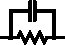
\includegraphics{graphics/logo_impedance}}
    }
  \end{center}
  \vspace{0.5cm}


  Interfacial double-layers link the two halves of this thesis and form the underlying theme.
  In~\cref{part:doubleLayersOnInsulators}, double layers are used as a means of converting fluid-mechanical energy into electrical energy.
  The primary application being an energy harvester that could power electronic water meters.
  Domestic water meters are typically installed where electrical connection is not feasible.
  Harvesting energy at the meter may make electronic metering a feasible long-term solution.
  My findings show that double layer based energy harvesters are not efficient enough for this application \emph{yet}.
  Recent literature on the subject suggests large gains in efficiency may be possible using more exotic materials.
  Such gains would allow a compact harvester to generate enough energy to operate an electronic meter with wireless transmitter.

  \Cref{part:doubleLayersOnConductors} models the electrical impedance of electrodes submerged in an electrolyte.
  Double-layers contribute to the electrical impedance between solid-fluid interfaces.
  This work is important to designers of medical implants; and by extension, anybody who relies on the implants themselves.
  Engineers use solutions of saline to mimic the environment experienced by their implants once implanted.
  This provides a way to test implant electronics without putting a patient at risk.
  A way of characterising the interface between electrodes and an electrolyte is to model it mathematically.
  An electrical of an electrode-electrolyte interface was recently developed by my supervisor, Jonathan Scott.
  I use that model to compare electrodes placed in solutions of saline to those placed in a living animal.
  Measurements of the two show that no one concentration of saline matches the situation inside a live spinal cavity.
  I then create a low-cost electrolyte test solution that better matches the impedance measured in a living animal's spinal cavity.

  % Edit checkpoint 2015-09-09 19:17

\phantomsection\addcontentsline{toc}{chapter}{Abstract}

\chapter*{Acknowledgement}
\phantomsection\addcontentsline{toc}{chapter}{Acknowledgement}
Thanks to Jonathan Scott (my chief supervisor), Steve Newcombe (Waikato University's award winning glass blower) and Peter Single (the senior electrical engineer at Saluda Medical) for their time, resources and patience.
Thank you to my second supervisor, Marcus Wilson, for checking up every so often and help proof-reading.
Thanks also go to the University of Waikato for funding the first three years of this work with a Waikato Doctoral Scholarship.
The support of my partner (Sarah) and my mother (Gina) has kept me on track during my research.
Lastly, thank you to everyone who has contributed to open-source projects, especially those part of:
\begin{itemize}
\item The Linux kernel and GNU tools
\item Gnome desktop environment
\item Inkscape vector drawing software
\item Gimp image manipulation program
\item The Arch Linux distribution
\item \TeX \space and its derivative \LaTeX
\item Python
\item ngSpice
\end{itemize}
Work done throughout this thesis has relied heavily on these tools.

\tableofcontents{}
\listoffigures
\listoftables
\doublespacing

%% Introduction

\pagenumbering{arabic}

 \chapter{Introduction}
   \label{chap:introduction_main}
   %!TEX root = ../../thesis.tex

\section{Background}
  Measuring and modelling the electrical properties of double layers draws on concepts from both elecronics and chemistry.
  This chapter is intended to give those readers unfamiliar with chemistry some essential background on the subject.
  We start with some general background on liquids and move toward definining what the double layer is.

  \subsection{Behaviour of liquid}
    Double layers are nothing more than an organised state of liquid.
    But before we discuss double layers it will be of benefit to put liquids themselves in perspective.
    After all, this thesis revolves around understanding its behaviour.

    Liquid behaviour is simple and calculable at the macroscopic scale.
    Modern computers can simulate the movement of liquids using the Navier-Stokes equations with accuracy and speed.
    This does not hold true when modelling fluid at the microscopic scale.
    Individual atoms and molecules interact with great complexity.
    Interactions are chaotic and simulation of any reasonable sized volume demands massive computing resources.

    \begin{figure}
        \begin{center}
            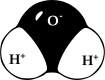
\includegraphics{content/introduction/graphics/polarWater}
        \end{center}
        \caption{Molecular diagram of a single water molecule}
        \label{fig:waterMolecule}
    \end{figure}

    Water is a liquid comprised of the molecule $H_{2}O$.
    A molecular diagram of water is shown in figure~\ref{fig:waterMolecule}.
    This molecule is polar, meaning one side has a net positive charge and the other has a net negative charge.
    This imbalance is responsible for very complex behaviour when dealing with a liquid body of any reasonable size.
    Water molecules can rotate and migrate so as to neutralise an electrical field.
    This means that a body of water, or any polar liquid, behaves as an extremely lossy transmission medium.

    We are concerned in particular with interactions occurring at the boundary between solids and liquids.
    This boundary is referred to as the interface.
    Interactions of interest here occur on the liquid side of the interface; in a very thin layer.
    This layer is known as an interfacial double layer.

    {\color{blue} Edited to here}
    
    The electric field of the solid's interior would be affected by the accumulation of charge at its surface, but this should not affect the analysis of the exterior layer.
    It is important to note that a solid in the context of this thesis is not simply the walls of a container, but may also refer to solid particles, even molecules, within a liquid.
    This is the case for emulsified substances such as paints where the formed double layer determines the stability of the emulsion.

    This thesis focusses on two applications of interfacial double layers with respect to electrical engineering. Firstly, it looks at a method of harvesting power from water by way of a mechanism that has no moving parts; and secondly, it models the electrical impedance that is seen by a medical implant when placed inside a biological system. The second application is where the majority of the research effort can be found.

  \subsection{Molecular simulation}
    Physical simulations involving the properties of materials and interactions with radio-waves are a common tool for any RF engineer. There are many areas in science and engineering that benefit from powerful computer simulation. Many modern-day computer games simulate the position and velocity of thousands of objects, such as bullets and buildings breaking apart, in near real-time.

    These kinds of simulations generally involve calculating the state of a system of objects at a specific time, then adjusting the all of the parameters based the physics of that system at a specific time, and repeating this process for as long as the simulation need continue.

    Finite-difference time-domain (FDTD) simulation is a common technique for calculating electrical fields and resulting currents and voltages in the field of electrical engineering. Such simulations can involve hundreds of thousands, \emph{sometimes millions}, of objects. Generally these objects are elements of a 3D mesh that has been created to represent the geometry of the system to be simulated. In such a simulation, each mesh element at every time step needs its various parameters (e.g. temperature, electromagnetic fields, electrical current and voltage) to be calculated based on the parameters of neighbouring objects in the mesh. Because of the dependence on neighbouring parameter values, each time-step may take many passes over each element in a system to calculate the final state before moving on. These sorts of simulations are extremely valuable for the radio frequency engineer as systems of a practical size can be simulated relatively quickly on modest computing hardware.

    At this point it seems natural to assume that we could model the behaviour of atoms and molecules in a liquid. Doing this would allow simulation of the interactions that take place at the fluid-soild boundary. It is possible to run such molecular dynamics (MD) simulations, however the number of atoms and molecules in any practical sized volume of fluid is astronomical.

    The molar mass of water is defined as $18.0528\thinspace g/Mol$, which represents the amount of water in moles per gram. One gram of water is defined as one millilitre so we can say that for every millilitre of water we have we have an eighteenth of a mole of water. Avagadro's constant, the number of constituent particles per mole of a given substance, is $6.0221\thinspace \times 10^{23}$. Therefore we have one eighteenth of Avagadro's constant in water molecules, which is about $3.3333\times 10^{22}$ molecules. That is 33 333 333 333 333 333 333 333 molecules! The behaviour of double layers in the applications of this research require a far greater volume than $1\thinspace ml$ to be useful, putting molecular simulation out of the picture for the applications discussed in this thesis for the foreseeable future.

  \subsection{Interfacial double layer}

    \begin{figure}
      \begin{center}
        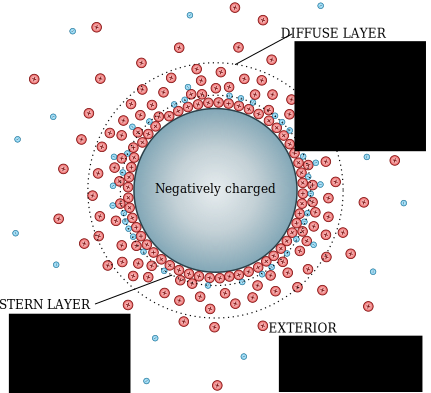
\includegraphics{content/introduction/graphics/doubleLayer_labelled.pdf}
      \end{center}
      \caption{Anatomy of the double layer}
      \label{fig:doubleLayer_anatomy}
    \end{figure}

    Double layers appear to varying degrees almost everywhere an electrolytic fluid and a solid are in contact. They are very small {Todo: quantify typical double layer sizes}, existing in the micro scale, and are responsible for a number of macro scale effects. Such effects are the stability of emulsions {Todo: find instances where double layers play a role}, the something else and even... They are a natural response when two systems of arrangement are brought to contact - fixed and fluid arrangements of charged particles.

  \subsubsection*{Physical Description}
    Double layer formation is the result of a liquid system responding to an imbalance of charge distribution. Atoms within a solid domain are static, they cannot repel each other or rearrange themselves. In a fluid the opposite is true, each freely moving charged entity will attempt to distance itself from others of like charge and move toward those of opposite charge. When these two domains are brought into contact with one another, the one whose elements are free to move (the liquid), moves to accommodate the imbalance in charge between the two domains. The effect of which is that an electrolytic liquid attracts atoms and molecules with a net opposite charge to the surface of the solid.

  \subsubsection*{Formation}
    {\color{blue}
    In order for a double layer to form, the liquid phase must contain ions, charged molecules, or polar molecules.
    This means there are likely to be non-participating elements within the fluid, that is, elements not affected by the charge {Todo: check affected and effected} of surrounding elements.
    The reverse case is also true {Todo: is this correct?, I just made it up} where an electrolyte solution comes in contact with a electrically neutral and stable solid. Although this case is not as obvious as one may think. For example, placing pure water in a glass flask, it may be assumed, would not cause the formation of a double layer. Glassware in used throughout chemistry laboratories as it reacts with very little and pure water with no salt ions should be fairly stable. This is not the case however as glass in contact with water undergoes a process of deprotonation at the boundary. This deprotonation is where $H^{+}$ ions are torn from the surface of the glass and enter the liquid phase. As this happens, the surface of the glass is left negatively charged. Subsequently, a double layer is formed from polar water molecules and hydrated protons.
    }



    Figures \ref{fig:doubleLayer_set1} and \ref{fig:doubleLayer_set2} illustrate the formation of such a layer around a charged object that, for the sake of illustration, instantaneously appears in a settled electrolyte solution. In these figures, the spacing of depicted fluid elements do not represent the density of a liquid system and the smooth surface of the charged object in no way resembles the surface of a solid at the scale of individual atoms.

    The first set of images, figure \ref{fig:doubleLayer_set1}, depict charged elements in the fluid responding to the presence of the solid by aligning themselves with the induced field and migrating toward or away from the object. The second set of images, figure \ref{fig:doubleLayer_set2}, shows continued migration of charged particles and the formation of the Stern layer at the solid-liquid interface. Members of this layer are bound so strongly to the object that they are effectively immobile, i.e., they are adsorbed to the solid object. A substantial proportion of the initial electrical field from the solid is shielded by the Stern layer.

    Outside the Stern layer, as the field strength continues to diminish with increasing radial distance, ions and molecules are attracted with decreasing strength. This reduction in attraction forms a layer that is thicker than the stern layer and mobile; the ions are free to move locally within this secondary layer. This secondary layer is called the diffuse layer and it is convenient to visualise it as a fluffy cloud of charged particles attracted to, but not trapped upon, the thin Stern layer immediately adjacent to the surface.

    \begin{figure}
      \begin{center}
        \includegraphics{content/introduction/graphics/doubleLayer_t0.pdf}
        \includegraphics{content/introduction/graphics/doubleLayer_t1.pdf}
        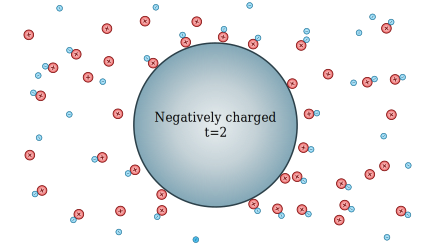
\includegraphics{content/introduction/graphics/doubleLayer_t2.pdf}
      \end{center}
      \caption{Creation of a double layer (time 0-2)}
      \label{fig:doubleLayer_set1}
    \end{figure}

    \begin{figure}
      \begin{center}
        \includegraphics{content/introduction/graphics/doubleLayer_t3.pdf}
        \includegraphics{content/introduction/graphics/doubleLayer_t4.pdf}
        %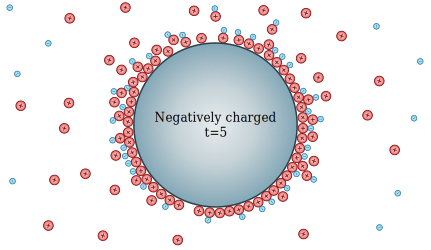
\includegraphics{content/introduction/graphics/doubleLayer_t5.pdf}
        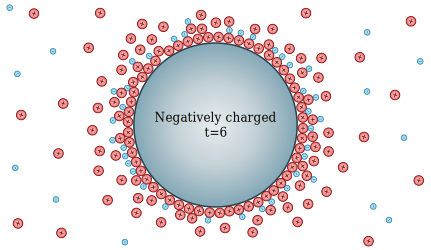
\includegraphics{content/introduction/graphics/doubleLayer_t6.pdf}
      \end{center}
      \caption{Creation of a double layer (time 3-6)}
      \label{fig:doubleLayer_set2}
    \end{figure}


  \subsubsection*{Electrical Behaviour}

\section{Motivation}
  This thesis begins with the question: is it possible to harvest enough electrical energy from flowing water, without moving parts, to power a smart meter?
  The logic being that a harvester without moving parts would last longer than its mechanical equivalents.
  I started by investigating an assortment of possible mechanisms (discussed in detail in Chapter

  I started by investigating
  \begin{itemize}
    \item piezoelectric vibrators,
    \item electrostatic generators, and
    \item streaming potential cells
  \end{itemize}
  as potential harvesting mechanisims.

  The piezoelectric vibrator was the equivalent of a water whistle with a vibrational energy harvester attached.
  The electrostatic generator was a version of Lord Kelvin's Electrostatic Generator with a harvesting application.
  The streaming potential cell was a mystery.

  We knew geologists used streaming potentials to measure underground water flow.
  All we knew about the mechanism was that forcing water through something generated a voltage somehow.
  It was learning about that mechanism and answering the following questions that started me on what became this thesis.
  \begin{enumerate}
    \item Where does the streaming voltage come from?
    \item What role does the geometry of the device play?
    \item Could you change the materials to get more voltage?
  \end{enumerate}
  I eventually concluded that streaming cell harvesters were not practical for our application.
  By this time I had a working knowledge of interfacial double layers and their properties.

  My supervisor, Jonathan Scott, was on a sabbatical at Saluda Medical working with implant electrodes.
  There he developed an electrical model of the impedance presented by electrodes immersed in a solution of saline.
  This model would predict the electrical impedance seen between two electrodes when implanted in the spine of a human.
  Most of the behaviour the model reproduced was a result of interfacial double layers.

  Saluda wanted to know how good a substitute saline was for spinal fluid with regards to electrical impedance.
  There was no way to know and no way to compare solutions, except for using the new model.
  I took the model and started the next stage of my research; characterising fluids based on the impedance they present to electrodes.
  I was able to leverage my understanding of interfacial double layers and apply it to medical engineering.

\section{Publications}

\section{Thesis Outline}


% Edit checkpoint 2015-09-09 20:52

 \chapter{Backgound}
   \label{chap:background}
   %!TEX root = ../../thesis.tex


\section{Double Layers}
  \label{sect:background_doubleLayers}


  Modelling and measuring the electrical aspects of interfacial double layers draws on both electronic and chemical concepts.
  Those with an electronic background are unlikely to be familiar with double layers.
  This section provides background on what a double layer is and how one is formed, beginning with a discussion of liquids.


  \subsection{Formation}
    \label{sub:background_doubleLayers_formation}


    % Water
    \begin{figure}
        \begin{center}
            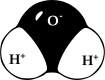
\includegraphics{content/introduction/graphics/polarWater}
        \end{center}
        \caption{Molecular model of the water molecule}
        \label{fig:waterMolecule}
    \end{figure}
    A double layer is an organised layer of liquid; two layers to be precise.
    Because double layers are a property of liquids, and most common liquids are water based, the properties of water is an appropriate place to start.
    These properties of are not necessary for the formation of double layers, but knowing of them helps build a mental model of the surrounding system.
    At the microscopic scale, individual atoms and molecules within liquids interact with complexity.
    The density of atoms and molecules in water is extreme, $3.33\times10^{22}$ \ce{H2O} molecules per millilitre.
    These molecules are polar, meaning that one side appears negatively charged while the other appears positively charged, shown in~\cref{fig:waterMolecule}.
    This causes them to respond to electric fields by rotating, so as to minimise their potential energy in the field.
    Because of this, any ions present become surrounded by arranged volumes of water.
    For example, a positive ion will be surrounded by water molecules orientated such that their hydrogen atoms all point away from the ion.
    It is also possible for water to spontaneously disassociate from \ce{H2O} into a proton (\ce{H+}) and a hydroxide anion  (\ce{OH-}).

    % Formation
    To form a double layer a liquid containing ions must meet a solid object with charged trapped at its surface.
    Once this happens, the ions within the liquid are drawn to, or repelled from, the solid's surface.
    The point where the two states of matter meet is called the interface.
    Those ions that have been drawn to the interface collect together to form a double layer.
    Double layers occur when using pure water as the liquid, because of its ability to disassociate, but mostly it is the ions from an electrolyte solution that form the layer~\cite{Bruesch2004}.
    The double layer is simply the collection of ions drawn from a liquid to the surface of a solid.


    % Shielding
    \begin{figure}
        \begin{center}
            
\includegraphics[scale=0.8]{content/introduction/graphics/butterfat}
        \end{center}
        \caption{Structural formula of a butterfat molecule}
        \label{fig:butterfat}
    \end{figure}
    A solid solid may refer to the walls of a container or particulates suspended in solution.
    When a particulate is suspended throughout a solution it is referred to as an emulsion.
    For example, milk is such an emulsion of butterfat in water.
    \Cref{fig:butterfat} shows the structure of a butterfat molecule; a long structure that behaves as a solid.
    The stability of an emulsion, such as milk, depends on the strength of the double layers that encapsulate each particle.
    These double layers shield the molecules or particles from one another electrically.
    By shielding them from each other they are unable to collect and bond together.
    This shielding prevents milk from coagulating and turning to lumps.

    %% Interfaces
    %\begin{figure}[h]
        %\begin{center}
            %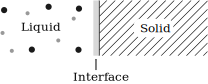
\includegraphics{content/introduction/graphics/simpleLayerDiagram}
        %\end{center}
        %\caption{Diagram showing the location of the fluid-solid interface}
        %\label{fig:interfaceDiagram}
    %\end{figure}
    %The boundary between any two states of matter is referred to as an interface; it is simply where two things meet.
    %We are interested specifically in the dynamics of the solid-liquid interface.

    %Interactions relevant to double layers occur in a thin region inside the liquid at the interface.
    %When there is a difference in charge between the solid surface and the liquid bulk, a double layer forms.
    %The following three statements are capture underlying nature of double layers.
    %\begin{itemize}
      %\item The charged elements in a solid are fixed in place, but in a liquid they are free to move.
      %\item Any charge imbalance between solid and liquid will be greatest at the point they meet.
      %\item Charges interact with each other, whether by repulsion or attraction.
    %\end{itemize}
    %The consequence being that any charge interactions will be most pronounced within the liquid phase at the surface of the solid.


    Having addressed where double layers come from, as well as their organisation, the anatomy of these layers is now introduced.


  \subsection{Physical Model}
    \label{sub:background_doubleLayers_physicalModel}


    \begin{figure}
      \begin{center}
        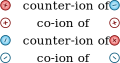
\includegraphics{content/introduction/graphics/counterAndCoIons}
      \end{center}
      \caption{Counter-ions are oppositely charged, co-ions have like charge.}
      \label{fig:counterAndCoIons}
    \end{figure}
    In the previous section, a brief explanation of what a double layer is and where they form was introduced.
    We next look at double layer anatomy and define some of its properties.
    Before moving on, use of the terms `co-ion' and `counter-ion' is defined.
    These terms refer to ions containing charge -- like or opposite -- in polarity to a second charge or body of charge.
    For example, if a negatively charged surface attracts positively charged ions then positive ions are the counter-ion.
    Likewise, if a positively charged surface was to repel a positive ion then the positive ion is the co-ion.
    The terms are convenient because they remove the need to identify specific polarities in discussion.
    This relationship is shown in~\cref{fig:counterAndCoIons}.

    \begin{figure}
      \begin{center}
        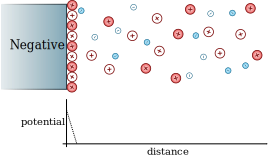
\includegraphics{content/introduction/graphics/model_helmholtz}
      \end{center}
      \caption{Structure of the Helmholtz layer.}
      \label{fig:doubleLayerModel_helmholtz}
    \end{figure}
    Three models of the interfacial double layer have been proposed over time.
    Each represents an extension or modification of the previous, beginning with the Helmholtz Model~\cite{Horch2004}.
    Helmholtz proposed his parallel plate capacitor based model in 1879~\cite{Geddes1997}.
    His model consists of two layers of surface charge, one inside the solid and one in the liquid.
    The counter-ions sit in a \emph{compact layer}, meaning that they are bound to the surface and immobile.~\cite{Salieb-Beugelaar2009}
    Figure \ref{fig:doubleLayerModel_helmholtz} represents this as a row of tightly packed positive ions along the solid surface.
    Past the layer of bound surface ions there is no affect from the charged surface of the solid.
    In essence, his model defines the interface a single layer of ions held against the edge of a solid.
    The problem with this model is its inability to predict the layer's capacitance.
    Measurement of a double layer's electrical capacitance changes depending on either the electrical potential across the layer, or the concentration of ions in the solution~\cite{Bard1980}.
    The Stern model does not account for this variation.

    \begin{figure}
      \begin{center}
        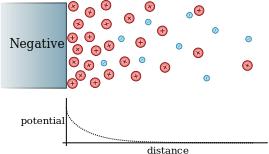
\includegraphics{content/introduction/graphics/model_guoyChapman}
      \end{center}
      \caption{Structure of the Goüy-Chapman layer.}
      \label{fig:doubleLayerModel_gouyChapman}
    \end{figure}
    Later, Goüy and Chapman independently proposed that charge in the liquid phase may instead be held in a \emph{diffuse layer}~\cite{Chapman1913}.
    This meant that ions in the layer were not fixed and that the density of charge in the layer could vary.
    Figure~\ref{fig:doubleLayerModel_gouyChapman} illustrates the concept by the lack of ions bound to the surface and the gradual decline in counter-ion concentration with distance from the surface.
    The Goüy-Chapmam Model accounts for the observed variation in capacitance by distributing charge in the liquid as a gradient from the surface of the solid.
    The layer is free to change its concentration profile in response to applied electrostatic potential and ionic concentration.
    In the case of a higher electrostatic potential, the layer is pulled closer to the surface, becoming shallower.
    In the case of a higher electrolytic concentration, the layer is more concentrated with a higher charge density, again becoming shallower.
    It predicts the change in capacitance by growing or shrinking the size of the layer, but it still fails to predict the capacitance at high ionic concentrations.
    This is in part because it fails to account for the physical size of the ions in the electrolyte and instead models them as point charges~\cite{Bard1980}.
    In their model, ions can get infinitely close to the surface regardless of their size.
    This becomes a problem at high ionic concentration where the surface becomes crowded.

    \begin{figure}
      \begin{center}
        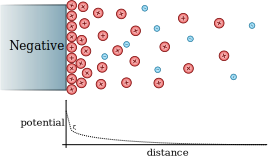
\includegraphics{content/introduction/graphics/model_stern}
      \end{center}
      \caption{Structure of the Goüy-Chapman-Stern layer.}
      \label{fig:doubleLayerModel_stern}
    \end{figure}
    In 1924, Otto Stern published his modified version of the Goüy-Chapmam model~\cite{Stern1924}.
    This model, illustrated in figure~\ref{fig:doubleLayerModel_stern} extends the Goüy-Chapmam model by setting the minimum distance an ion can get to the solid surface.
    This effectively reintroduces the compact layer as seen in Helmholtz's model but allows for a concentration gradient exterior to this layer.
    It resembles the Helmholtz model at high ionic concentration but accounts for spread in the layer dimensions at lower concentrations.
    The Stern, sometimes referred to as the Goüy-Chapmam-Stern, model is a well accepted double layer model~\cite{Olthuis2005}.


  \subsection{Anatomy}
    \label{sub:backgound_doubleLayers_anatomy}


    \begin{figure}
      \begin{center}
        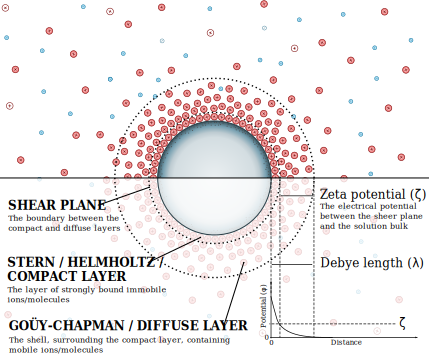
\includegraphics{content/introduction/graphics/doubleLayer_version2}
      \end{center}
      \caption{Anatomy of the double layer}
      \label{fig:doubleLayer_anatomy}
    \end{figure}
    Figure~\ref{fig:doubleLayer_anatomy} shows the double layer organisation according to the currently accepted Goüy-Chapmam-Stern model.
    It shows the compact layer adsorbed to the surface of the suspended solid.
    In this layer the ions are immobile due to the electrical strength at the surface.
    Surrounding this layer is the diffuse layer.
    Ions here are still drawn to the solid, but not so strongly as to be immobile.
    The electric potential in this layer decays from that within the compact layer to the potential in the bulk of the solution.
    These layers are divided by the shear plane.
    The shear plane represents nearest distance from the surface at which the layer can move laterally.
    This is an important parameter with linear geometries, such as the inside of a pipe, as it represents the true no-slip boundary.
    The thickness of a typical double layer is between \SI{1}-\SI{100}{\nano\meter}~\cite{Jiang2010}, as defined by its Debye length~\cite{Israelachvili2011}.
    The Debye length is the distance between the interface and the point in the liquid where the electric potential is no longer affected by the charged interface.
    As mentioned in the previous section, this varies based on the ionic concentration of the solution and the potential at the solid surface.


  % Marcus Wilson tore this apart, don't even mention computer simulation.
  %\subsection{Liquid simulation}
    %\label{sub:molecularSimulation}


    %At the macroscopic scale, liquid behaviour is simple and calculable.
    %Modern computers can simulate the movement of liquids using the Navier-Stokes equations with accuracy and speed.
    %Engineers simulate the flow of liquids, or any Newtonian fluid, routinely using computer design tools.
    %These tools allow engineers to push boundaries of aircraft and boat design.
    %However, this does not hold true when modelling fluid at the microscopic scale due to the required scale.
    %%Computer simulations are  based upon calculating the state of a system of objects at specific time intervals.
    %%There are other methods, such as
    %%At each computed time interval the variables of each element of a system are updated and the cycle repeats.
    %%This repeats for every time-step until the simulation time-frame has run its course.
    %%These simulations are not run in real-time; instead taking hours or days to compute simulations spanning fractions of a second.

%%    Finite-difference time-domain simulation is a common technique for calculating electrical fields and resulting currents and voltages in the field of electrical engineering.
%%    Such simulations can involve hundreds of thousands, \emph{sometimes millions}, of objects.
%%    These objects are elements of a 3D mesh created to represent the geometry of the system.
%%    Because of the dependence on neighbouring parameter values, each time-step may take many passes over each element in a system to calculate the final state before moving on.
%%    This type of simulation is common whenever the effects of radio waves need to be simulated.

    %Designing and conditioning computer simulations at a molecular scale are challenging.
    %Simulating the interface is possible, but is very involved and constitutes a field of its own.
    %The work of Nagy et al.\ ~\cite{Nagy1992} and Bazant et al.\ ~\cite{Bazant2011} has shed light on some of the underlying physical mechanics of the double layer.
    %Matters are complicated by the fact that some aspects of the double layer are still not fully understood~\cite{Kornyshev2007}.

    %Simulation of a liquid having a sensible macroscopic volume is impractical.
    %The molar mass of water is \SI{18.0528}{\gram\per\mole}.
    %One gram of water is defined as one millilitre, so we can say that for every millilitre of water we have we have an eighteenth of a mole of water.
    %Avagadro's constant, the number of constituent particles per mole of a given substance, is $6.0221\thinspace \times 10^{23}$.
    %Therefore we have one eighteenth of Avagadro's constant in water molecules, which is about $3.3333\times 10^{22}$ molecules.
    %Molecular simulation has not been employed here.
    %Useful results are likely to be obtained from volumes less than \SI{1}{\milli\litre}, but the time and resources to successfully run and validate such simulations are high.
    %Such simulations are shaping the underlying models of the interfacial double layer~\cite{Kornyshev2007}.


\section{Streaming Cells}
  \label{sect:background_streamingCells}


  % Double layes on flat surfaces
  \begin{figure}
      \centering
      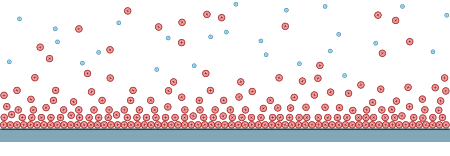
\includegraphics{content/pt1/01-PowerHarvesting/graphics/intro_2_wall}
      \caption{
        \label{fig:doubleLayerBetweenWalls}
        Formation of a double layer along a solid wall.
      }
  \end{figure}
  Consider a double layer that has formed along a perfectly flat surface.
  \Cref{fig:doubleLayerBetweenWalls} illustrates this situation, where the walls are negatively charged and therefore the counter-ions are positively charged.
  Counter-ions, separated from the bulk of the liquid, line the exterior of the wall; but charge separation is not enough to generate electrical power.

  % Harvesting energy
  \begin{figure}
      \centering
      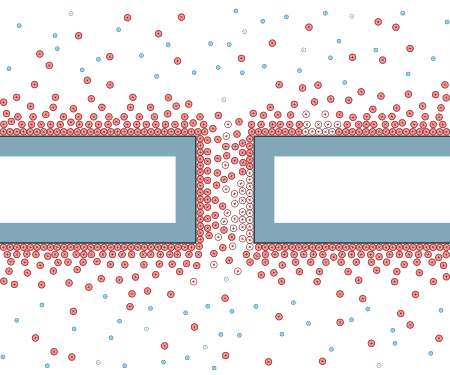
\includegraphics{content/pt1/01-PowerHarvesting/graphics/intro_2_channel_relaxed}
      \caption{
        \label{fig:doubleLayerInChannel_noPressure}
        Double layer formation within a streaming cell that is in a state of equilibrium.
      }
  \end{figure}
  Energy can not be created or destroyed, it must be converted from one form to another.
  In this case, counter-ions are electrostatically bound to the interface and removing them requires work.
  Although the counter-ion density has been increased at the boundary, the charge is not free.
  Migration of charge to the walls ceases once the surface potential has been neutralised.
  Double layer formation takes work to undo and the process stops once the layer is formed.
  Generating electrical energy requires taking some form of power from the fluid, in this case mechanical.
  Liquids pass mechanical power in the form combination a pressure and a flow.
  Harvesting power from liquid will cause a drop in pressure as liquid is pushed through the harvesting mechanism.
  The mechanisms presented here use mechanical power to shift the ionic balance between two bodies of liquid.
  This means separating and isolating negative and positive ions from each other.
  Figure~\ref{fig:doubleLayerInChannel_noPressure} shows another charged wall, but with the addition of a small channel.
  Notice that the channel contains no co-ions, it is exclusively occupied by counter-ions.
  The ratio of counter-ions to co-ions within the channel is controlled by the width of the channel.
  The narrower the channel, the less likely it is for co-ions to get inside.
  This channel is small enough that the layers overlap one another, repelling co-ions.
  The channel and the two separated bodies of liquid now form an energy harvester.
  Counter-ion rich fluid is transported across the channel by applying a pressure differential.
  As counter-ions exit the channel on the low-pressure side, new ions move to replenish the double layer on the high-pressure side.
  \begin{figure}
      \centering
      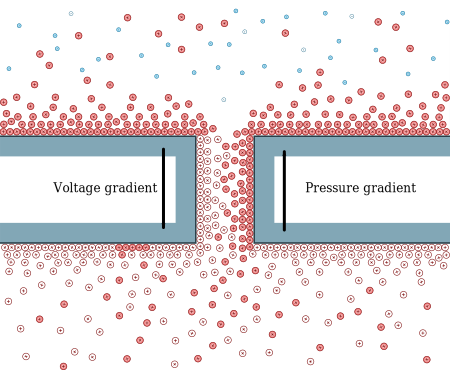
\includegraphics{content/pt1/01-PowerHarvesting/graphics/intro_2_channel}
      \caption{\label{fig:doubleLayerInChannel_withPressure}Double layer formation within a streaming cell that has a pressure differential applied.}
  \end{figure}
  A diagram showing the channel geometry, but with pressure applied and a voltage gradient generated is shown as figure~\ref{fig:doubleLayerInChannel_withPressure}.
  The, including the non-conductive wall, is referred to as a streaming cell.
  Streaming cells are able to continuously separate ions of an electrolyte fluid.
  Electrical potential across a streaming cell increases as those ions are pumped through.
  This only works when the solid surface has charge at its surface, necessary to form the double layer.

  % Channel fabrication and materials
  A channel can be created individually using a range of fabrication methods, such as chemical etching or using narrowly separated parallel plates.
  They can also be formed en masse by using porous materials such as glass or ceramics, where the pores themselves act as channels.
  Glass has the convenient property that it spontaneously obtains a negative surface charge when in contact with water, the requirement for double layer formation.
  This surface charge is caused by the deprotonation of surface silanol groups in glass (SiOH~$\leftrightarrows$~SiO$^{-}+$~H$^{+}$)~\cite{Kirby2004}.
  By immersing a glass channel in an electrolyte solution, the glass donates protons into the solution leaving its surface negatively charged.
  In turn, positively charged double layers line the channel's inner walls ready to be pumped through the channel.
  This means that glass channels have a higher voltage on the low-pressure side and a lower voltage on the high-pressure side.

  % Limitations of previous content
  The concept behind the device is relatively straight-forward, but the physical reality is complex.
  The diagrams presented here are simplified, having perfectly flat walls containing single atom ions carrying a single charge.
  No mention of molecules has been made, which increases the complexity.
  Polar molecules such as water have positive and negative components offset in space.
  Although simplified, this material illustrates the how streaming cells work.
  Next, literature concerning the operation, design and improvements to streaming cell technology is presented and discussed.


  \subsection{Literature Review}
    \label{sub:background_streamingCells_literatureReview}


    % Initial work of Osterle
    \begin{figure}
      \centering
      \includegraphics[height=6cm]{content/pt1/Osterle_ElectrokineticCell.png}
      \caption{\label{fig:Osterle_cell}Osterle's electrokinetic pumping cell, reproduced from \cite{Osterle1964}}
    \end{figure}
    In 1964, a paper by Osterle gave an analysis of energy conversion from streaming cells, both for the purpose of pumping fluid or generating electrical power was presented~\cite{Osterle1964}.
    The cell he used consisted of fine capillary tubes stacked together to form a streaming cell.
    A diagram of that cell, in its pumping configuration, is reproduced here as~\cref{fig:Osterle_cell}.
    Importantly, he shows that a streaming cell has the same conversion efficiency whether it is in a pumping mode, where electrical energy is supplied, or in a generating mode, where electrical energy is produced.
    Based on his analysis, Osterle gives an illustrative example of an streaming cell producing electrical energy.
    He states that tube bank having a volume of \SI{100}{\centi\meter\cubed} with \SI{100}{\kilo\pascal} of hydrostatic pressure applied would be capable of producing \SI{0.49}{\watt} of electrical energy.
    This would require \SI{125}{\watt} of pumping power to achieve, giving an energy conversion efficiency of \SI{0.392}{\percent}.

    % Another, paper - the beginning of streaming cells
    Within the space of a year three papers related to properties of fluid flow in fine capillaries, such as those used by Osterle are presented.
    Burgreen and Nakache investigate both the flow when the capillaries are rectangular~\cite{Burgreen1964}, and the efficiency of such capillaries when used to generate electrical power or to pump~\cite{Burgreen1965}.
    Their work develops mathematics behind rectangular streaming cells and shows fine glass capiliaries are equally efficient when used to generate electrical power or to induce liquid pumping.
    Rice and Witehead make an analysis of fluid flow profiles that consider the effect of double layer interactions~\cite{Rice1965}.
    They show how the double layer affects the level to which liquid can permeate a material populated with cavites.
    Together these three papers mark the beginning of research into streaming cells.

    % Renewed interest and dimensions
    There appears to be little published research into streaming cells until 2003, when a surge of papers related to optimal dimensions of streaming cells appear.
    An analysis relating energy conversion efficiency to the length of a streaming cell channel indicated that short cells are the most efficient~\cite{Yang2003}.
    However, more recent work by Chang and Yang shows a decrease in conversion efficiency at maximum power when the channel length is low~\cite{Chang2009}.
    This work suggests there is an optimum channel length, which is also dependent on the fluid conductivity.
    Investigation into the relationship between the Debye length of the double layer and streaming cell conversion efficiency found that a channel is most efficient when its height is twice that of the Debye length~\cite{Daiguji2004}
    This corresponds to the point at which double layers formed within a cell begin to overlap with one another.

    In 2005 a seminal paper by van der Heyden et al.\ reported on streaming cell measurements made in a single micro-channel \SI{70}{\micro\meter} in height~\cite{VanderHeyden2005}.
    Many valuable contributions were detailed in this paper, namely:
    \begin{enumerate}
      \item Confirmed that reversing the polarity of surface potential reverses the direction of the streaming current.
      \item Found that the maximum conversion efficiency corresponded to channels where double layers begin to overlap. This confirms the relationship put forward the previous year by Daiguji et al.\
      \item Show that boundary conditions involving constant surface potentials, used up to this point to model streaming, are inaccurate.
      \item Predict a maximum energy conversion efficiency of $\sim$\SI{6}{\percent} for potassium chloride solutions of \SI{1e-5}{\mole} in silica channels of height \SI{145}{\nano\meter}.
    \end{enumerate}
    Subsequent research by the same authors reported that energy conversion efficiency is maximised at low salt concentrations~\cite{VanderHeyden2006}.
    In which they predicted a \SI{12}{\percent} efficiency for streaming cells using electrolyte solutions of lithium.
    Around the same time, Daiguji et al.\ publish work suggesting that in order to increase cell efficiency one may either reduce the channel height or decrease the ionic concentration of the working fluid~\cite{Daiguji2006}.
    This supports the work of van der Heyden et al.\ with respect to efficiency gains with the working fluids having low ionic concentrations.

    % Stern conductance
    In 2007, van der Heyden et al.\ publish a measured energy conversion of \SI{3.2}{\percent}~\cite{Heyden2007}.
    They suggest that the conversion efficiency of a channel is limited by a property termed `Stern conductance'.
    The concept of Stern conductance is that the Stern layer (see \cref{fig:doubleLayer_anatomy}) itself provides a pathway for electrical conduction.
    This conduction turns the surface of the glass into an electrically conductive surface causing the cell to partially self-discharge.
    Stern conductance is often referred simply as `surface conductance'.
    Davidson and Xuan published a mathematical model shortly after confirming the role of Stern conductance on streaming cells, in particular those with low ionic strength~\cite{Davidson2008}.
    They suggest that this is the reason for poor measured efficiencies in light of the much higher predicted values.

    % Hydrodynamic slip
    \begin{figure}
      \centering
      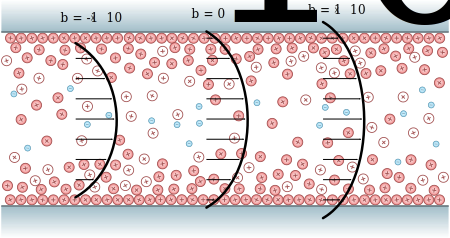
\includegraphics[height=6cm]{content/pt1/graphics/HydrodynamicSlip}
      \caption{\label{fig:HydrodynamicSlip}Illustration of hydrodynamic slip inside a channel cavity, where $b$ is the slip length. Arrows indicate flow velocity in each of the three situations.}
    \end{figure}
    Most recently, the concept of hydrodynamic slip has been applied to streaming cells as a way of increasing conversion efficiency.
    Estimates using mathematical models predicted conversion efficiencies between \SI{30}{\percent} and \SI{70}{\percent}~\cite{Pennathur2007, Davidson2008a, Ren2008}.
    Hydrodynamic slip refers to the ability of a fluid to `slip' relative to a boundary/interface.
    Slip is advantageous to streaming cells because it permits ions in the Stern layer to move relative to the wall.
    The length refers to an imaginary distance into the solid wall where the traditional `no-slip' boundary condition would occur (refer to~\cref{fig:HydrodynamicSlip}).
    A `no-slip' boundary condition dictates that fluid at the boundary of a solid must have zero velocity.
    This condition, along with viscosity, is responsible for the parabolic flow profile a fluid takes as it moves through pipes.
    An issue surrounding slip was illustrated by Eijkel who showed that a channel's zeta potential and its slip length are linked~\cite{Eijkel2007}.
    The general problem with slip-based mechanisms is that a high zeta potential is optimal for double layer formation, however it also promotes wetting.
    Wetting and hydrodynamic slip are related to each other by the strength of attraction between a liquid and a solid.
    To explain, the terms hydrophobic and hydrophilic are used to describe surfaces that repel and attract water.
    A hydrophobic surface has a low tendency to support water, i.e., water will bead and roll off a hydrophobic surface.
    Conversely, a hydrophilic surface is one that water \emph{is} attracted to, causing a droplet to spread and stick to the surface.
    Hydrodynamic slip occurs when a channel's walls are hydrophobic, allowing water at the interface to slip along the boundary of the solid.
    High zeta potentials attract water to the solids surface due to electrostatic attraction.
    Eijkel's publication illustrates that the zeta potential and hydrodynamic slip are related to one another.
    In order to improve the situation in steaming cells a surface should be both non-wetting and hold a high surface charge.
    Conservative estimates place an efficiency of \SI{40}{\percent} on cells having slip lengths tens of nanometres long, obtainable using carbon nanotubes, using solutions having low salt concentration.


    %Research around streaming cell energy conversion headed in a new direction after an article written by Pennathur et al.\ in 2007 detailed a mathematical model predicting the effects of hydrodynamic slip~\cite{Pennathur2007}.
    %It proposed efficiency figures as high as \SI{30}{\percent} for a slip length of \SI{6.5}{\nano\meter} in cylindrical tubes \SI{100}{\nano\meter} in diameter.


    %Eijkel, in a follow-up publication to that of Pennathur's, discusses the relationship between zeta potential and slip length~\cite{Eijkel2007}.

    %\begin{figure}
      %\centering
      %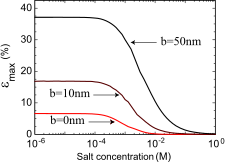
\includegraphics[height=6cm]{content/pt1/graphics/SteinSlipEnchancedChannelEfficiency}
      %\caption{\label{fig:Stein_Slip_Prediction}Plot of predicted efficiency versus salt concentration for various for slip lengths of 0, 10 and \SI{50}{\nano\meter}, taken from~\cite{Ren2008}.}
    %\end{figure}

    %That same year, two papers modelling the effects of hydrodynamic slippage were published.
    %The first, by Davidson and Xuan, gives a mathematical prediction of the effects of hydrodynamic slippage at the interface surface~\cite{Davidson2008a}.
    %They predict that when taking slip at the solid-fluid boundary into consideration that conversion efficiencies as high as \SI{30}{\percent} should be obtainable.

    %The second, by Ren and Stein, predict conversion efficiencies as high as \SI{70}{\percent} based on the slip lengths recently observed with carbon nanotubes~\cite{Ren2008}.
    %They provide a more conservative prediction of \SI{40}{\percent} for slip lengths in the tens of nanometers region and low salt concentration.

    % Summary
    Theoretical predictions of the efficiency of standard micro/nano-fluidic channels are 2\% for pure water and 7\% for sodium chloride.~\cite{VanderHeyden2006}
    However, measured conversion efficiencies as reported thus far are:
    \begin{itemize}
      \item ``far less than \SI{1}{\percent}'' forcing potassium chloride through a porous glass plug having pores in the range \SI{1}--\SI{1.6}{\micro\meter}~\cite{Olthuis2005}.
      \item 0.01\% by forcing water through porous glass with pore sizes from 10\thinspace--\SI{16}{\micro\metre}.~\cite{Yang2003}
      \item 0.8\% by forcing pure water through a ceramic rod populated with \SI{6}{\micro\metre} pores.~\cite{Yang2004}
      \item 3\% by forcing a sodium chloride solution through a \SI{75}{\nano\metre} by \SI{50}{\micro\metre} silica channel.~\cite{Heyden2007}
      \item 0.77\% by forcing a sodium chloride solution through a \SI{200}{\nano\metre} pore in an alumina membrane.~\cite{Lu2006}
      \item 5\% by forcing a sodium chloride solution through a \SI{0.5}{\nano\metre} cylindrical pore in polyethylene terephalate foil.~\cite{Xie2008}
    \end{itemize}
    It is clear from the literature that there is significant progress to be made with respect to increasing the conversion efficiency of streaming cells.
    Techniques to induce hydrodynamic slip at the fluid-solid interface are predicted to increase this efficiency to 30-40\%~\cite{Davidson2008a, Ren2008}, but progress in this area is dictated by advancements in materials science.
    Experimental results utilising slip enhanced channels have not yet been reported in the literature.
    Surface enhanced channels will not be investigated due to manufacturing difficulty, cost, and the level of scientific development required to make progress.

    %In 2012, Cherng Hon et al.\ presented a novel method of producing electrokinetic power from steaming cells using salinity gradients~\cite{CherngHon2012}.
    %In this work the authors describe a system where flow through a conventional streaming cell is brought about by forward osmosis.
    %This allows the authors to generate electrical energy from streaming cells without mechanical pumping.
    %The application has limited use, but it highlights novel uses for streaming cells as a means of electrical generation.

    %Most recently, in 2014, Jiao et al.\ presented results showing that surface treatment of porous glass can increase conversion efficiency~\cite{Jiao2014}.
    %They show that ultrasonically pre-treating glass and subsequently applying Sodium Dodecyl Sulphate to the surface gave a relative increase of \SI{27.3}{\percent} in power density.
    %Unfortunately, they do not state the absolute efficiency of their channels in either case.

    %Theoretical predictions of the efficiency of standard micro/nano-fluidic channels are 2\% for pure water and 7\% for sodium chloride.~\cite{VanderHeyden2006}
    %Experimental results show conversion efficiencies in the range of:
    %These results indicate that small channels using solutions containing salt are more efficient.
    %According to \cite{Daiguji2004}, the efficiency is maximised when the channel height is twice that of the Debye length.
    %Additionally, ~\cite{VanderHeyden2006} states that the maximum efficiency is found when the salt concentration is low.

    In summary, the finding that maximum conversion efficiency occurs at low ionic concentration supports the use of tap-water as a working fluid.
    The use of glass as a substrate appears to be a suitable choice, which is both cost effective and a convenient material.
    The dimensions of cells found in the literature suggest fabricate trial cells is feasible with the equipment available.
    It appears that a conversion efficiency of \SI{0.01}{\percent} should be achievable using a porous glass plug.



\section{Impedance Modelling}
  \label{sect:background_impedanceModelling}

  \begin{figure}
    \begin{center}
      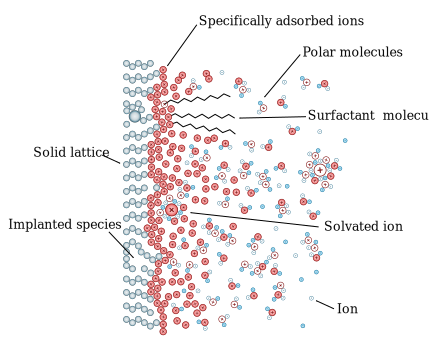
\includegraphics{content/introduction/graphics/interface}
    \end{center}
    \caption{Diagram of an liquid-solid interface showing various types of molecule configurations, surface imperfections and polar molecules. This diagram is based on the work of Bard et al. \cite{Bard1993}}
    \label{fig:interface}
  \end{figure}

  Most electronic components have well defined characteristics, such as impedance.
  This allows for the creation of circuit simulation tools, such as SPICE, that predict how a circuit will behave based on its description.
  Some electronic situations are not so well defined, meaning they can not be entered into circuit simulators.
  One such situation is when electrodes are inserted into an electrolyte.
  This would require the simulator to calculate the impedance through the electrolyte, but how do you calculate the impedance of an electrolyte bath?

  In \cref{sect:background_doubleLayers}, illustrations of double layers were presented showing that the interface is comprised of layers.
  A more realistic illustration of a solid-liquid layer is shown in \cref{fig:interface}.
  It shows interactions between polar molecules, between polar molecules and ions, surfactants at the interface, an imperfect solid/liquid boundary, and the the Stern layer.
  The complexity of interactions that happen at the interface are what make is so difficult to model.
  Additional to the interface's impedance is the geometry of the electrodes and the properties of the electrolyte.


  \begin{figure}
    \begin{center}
      \includegraphics{content/introduction/graphics/StJudeOctrode}
    \end{center}
    \caption{Drawing of an eight electrode array used for spinal stimulation. The electrode is called an Octrode and is made by St. Jude Medical.}
    \label{fig:octrode}
  \end{figure}

  To the designers of medical implant devices, estimating the impedance of electrodes in an electrolyte is critical for safe stimulator design.
  Saluda Medical is a young company based in Sydney, Australia, developing implantable spinal stimulators.
  Their engineers have designed a stimulator fit for human implantation, but are unsure of the electrical impedance that their implant will see once implanted.
  Getting it wrong could mean their microchip may `latch up'.
  This occurs when one or more pins on a chip goes higher than the supply voltage.
  When this happens, those pins that went above the supply voltage will get stuck on and the only way to turn them off again is to power down the entire chip.
  In an implanted setting this is potentially lethal.
  Naturally, Saluda want a way to model the impedance of electrodes implanted into a human spinal cavity.
  This involves modelling the electrode/electrolyte interface itself, a central idea in interface science.
  \Cref{part:doubleLayersOnConductors} of this thesis looks at ways of doing that using a model of the interface itelf.
  Such a model is suitable for entry into common circuit simulators, such as SPICE, that electronic engineers already use.
  


%% Part 1 - Energy Harvesting

\part{Double Layers on Insulators: Harvesting Energy}
   \label{part:doubleLayersOnInsulators}

   In \cref{sect:background_doubleLayers}, the topic of interfacial double layers were introduced.
   Then, in \cref{sect:background_streamingCells}, a way of utilising double layers to harvest energy - in a process called streaming - was studied.
   The possibility of using streaming cells as a means of powering electronic water meters is now put to the test.
   \Cref{chap:part1_streamingCellHarvesters} studies streaming cells, where some test cells are made and measured.
   With an understanding of readily available streaming cell performance, their applicability for use in water metering is discussed in \cref{chap:part1_waterMetering}.
   This presents an estimation of water use in a typical New Zealand home which is used to determine the amount of energy available to a harvester.
   \Cref{chap:part1_energyHarvestingRequirements} measures the energy consumption of low-power, 8-bit microcontrollers and wireless transmitters.
   The measured data is used to estimate the energy requirements of an electronic water meter with wireless transmitter.
   Finally, in \cref{chap:part1_conclusion}, the feasibility of using streaming cells as energy harvesters for our intended application is discussed and the conclusion is made.

   \chapter{Streaming Cell Energy Harvesting}
     \label{chap:part1_streamingCellHarvesters}
     %!TEX root = ../../../thesis.tex

This chapter begins with a mathematical analysis of streaming cells and operating parameters.
Then, in \cref{sect:part1_energyHarvesting_buildingStreamingCells}, a variety of streaming cell designs are built.
Early attempts at making streaming cells are presented, followed by more successful streaming cell designs.
Ten streaming cells are made using that design with each having slightly different geometric dimensions.
The electrical output and energy conversion efficiency of these cells is measured in \cref{sect:part1_energyHarvesting_measuringStreamingCells}.
Measurement results are discussed in~\cref{sect:part1_energyHarvesting_discussion}, followed by my concluding remarks.


\section{General Analysis}
  \label{sect:part1_energyHarvesting_generalAnalysis}


  A basic model of operation for a streaming cell is established.
  This determines what parameters are important when maximising a cell's output power.


  \subsection{Mathematics}


    Mathematical analysis of streaming cells provides a basic understanding of the parameters involved with their output and geometry.
    Rigorous mathematical analysis of streaming cell performance is extremely involved and is well detailed in the literature~\cite{Yang1998}.
    As aspects of a double layer's structure are still not fully understood, the mathematics behind them is still being developed.
    Computer simulation and mathematical models continue to shed light on ionic organisation at liquid-solid interfaces~\cite{Kornyshev2007}.
    For that reason, I have not attempted to model a streaming cell physically.
    Instead, I piece together a relatively simple mathematical model quantifying important operating parameters.


    \subsubsection*{Streaming voltage}

      Gu and Li derived the following equation relating the streaming voltage to the pressure applied across a streaming cell~\cite{Gu2000}.
      \begin{equation}
      \frac{V_{s}}{\Delta P} = \frac{\varepsilon_{r}\,\varepsilon_{0}\,\zeta}{\mu(\sigma+\frac{2}{\delta}\lambda)}
      \label{eq:part1_energyHarvesting_streamingVoltage}
      \end{equation}
      \noindent where:
      \begin{description}
          \item $V_{s}$ is streaming voltage
          \item $\Delta P_{z}$ is pressure differential (across the channel)
          \item $\epsilon_{r}$ is the relative permittivity of the liquid
          \item $\epsilon_{0}$ is the absolute permittivity of free space
          \item $\zeta$ is zeta potential
          \item $\mu$ is the fluid's viscosity
          \item $\sigma$ is the fluid's bulk conductivity
          \item $\delta$ is the channel's height
          \item $\lambda$ is the channel's surface conductivity
      \end{description}
      This equation is specific to parallel plate channels, of the type constructed in the following section.
      It requires that the width to height ratio of the channel is greater than 20, which it is for the cells constructed here.
      Gu and Li use this equation as a means of finding the zeta potential and surface conductance by rearranging it into the following form:
      \begin{equation}
        \frac{\varepsilon_{r}\, \varepsilon_{0}\, \Delta P}{\mu\, V_{s}\, \sigma} = \frac{1}{\zeta} + \left(\frac{2\, \lambda}{\zeta\, \sigma}\right)\, \frac{1}{\delta}
      \end{equation}
      Later, the streaming voltage of ten cells with the same dimensions of those used by Gu and Li will be measured.
      The left hand side of this equation will be plotted against the inverse of channel height to see if their results can be replicated.
      If successful, this will give a way of determining the zeta potential and surface conductance of the fabricated cells.


    \subsubsection*{Streaming current}


      Gu and Li, also also derive a similar equation for streaming current~\cite{Gu2000}.
      This equation, shown below, has been slightly rearranged to match the form of~\ref{eq:part1_energyHarvesting_streamingVoltage}
      \begin{equation}
          \frac{I_{s}}{\Delta P} = \frac{\varepsilon_{r}\,\varepsilon_{0}\,\zeta\,W\,\delta}{\mu\,L}
          \label{eq:part1_energyHarvesting_streamingCurrent}
      \end{equation}
      where
      \begin{description}
          \item $W$ is the width of the channel
          \item $L$ is the length of the channel
      \end{description}
      This equation is similar to that given by Olthuis et al.\ for a porous plug, but has been derived specifically for rectangular channels\cite{Olthuis2005}.


  \subsection{Electrical model}
    \label{sub:part1_energyHarvesting_generalAnalysis_electricalModel}


    % Model
    \begin{figure}
        \centering
            
\includegraphics[width=\textwidth]{content/pt1/01-PowerHarvesting/graphics/StreamingCell_EquivalentCircuit_output}
        \caption{\label{fig:StreamingCell_Schematic-representation}Schematic diagram of a streaming cell with connected load resistance.}
    \end{figure}
    Figure \ref{fig:StreamingCell_Schematic-representation} depicts schematically how a streaming cell operates when connected to an external load.
    A model of this sort is commonly used to analyse the behaviour transistors.
    This particular model is based on the work of Olthuis et al.\ in \cite{Olthuis2005}, but has been modified slightly.
    Instead of showing $\zeta$ as the equivalent voltage source, it is shown here instead with the pressure applied ($\Delta P$).
    This change was made because there is no way of controlling the zeta potential - it determined by the properties of the particular interface.
    However, the amount of pressure developed across the cell is controllable, and from \cref{eq:part1_energyHarvesting_streamingCurrent} it is shown to be directly proportional to streaming current.
    In fact, the transconductance ($g_{m}$) for this model is \cref{eq:part1_energyHarvesting_streamingCurrent}.
    The model aids analysis in that it shows the electrical configuration of an external load resistance ($R_{out}$).
    As shown, any load resistance placed across the cell is being placed in parallel with the internal electrical resistance of the cell.
    This will help to determine how best to optimise the cell in order to maximise its electrical output.


  \subsection{Optimisation}

    Having a mathematical model of a streaming cell allows for optimisation of its operating parameters.
    The model shows that any load placed across a streaming cell is actually placed in parallel with that cell's internal resistance.
    Therefore, choosing a suitable load is an important design consideration.
    It is possible to optimise the cell's output for maximum power output, or maximum efficiency.
    So which is best suited to harvesting applications?

    Streaming cells are not batteries.
    The only time energy can be extracted from a streaming cell is when pressure developed across it.
    This only happens because of liquid flowing through it.
    When harvestable power is available, we need to collect as much of it as possible -- \emph{no matter how much is wasted}.
    Because a cell is incapable of storing energy, any energy that we could not capture will be lost.

    The story would be different for battery applications.
    In those situations would be advantageous to optimise for maximum efficiency.
    Doing so will conserve the energy in a battery and ensure that as little as possible goes to waste.
    This might be something a cell phone designer aims to achieve, but is less important for batteries accelerating an electric car.

    In situations requiring maximum efficiency, the efficiency of the system approaches \SI{100}{\percent} as the power delivered approaches \SI{0}{\percent}.
    In situations requiring maximum power, the maximum achievable efficiency is \SI{50}{\percent}.
    This means we can only harness half of the electrical power developed by a cell, at best.


    \subsubsection*{Optimising $R_{out}$ for maximum power}


      Using Ohm's Law it is possible to form an equation linking the total power ($P_{cell}$) to the total electrical resistance across the cell ($R_{tot}$).
      \begin{eqnarray}
          P & = & V\times I\nonumber \\
          V & = & I\times R\nonumber \\
          P & = & I^{2}\times R\nonumber \\
          P_{cell} & = & I_{s}^{2}\times R_{tot}
          \label{eq:DeterminingOutputPower_basic}
      \end{eqnarray}
      Where $I_{s}$ is the streaming current created by pumping ions through the channel.
      As the output resistance and internal cell resistance are in parallel we can find the output current ($I_{out}$) by treating the cell as a resistor divider (as is shown in~\cref{fig:StreamingCell_Schematic-representation}).
      Using a resistor divider equation for current in parallel branches yields:
      \begin{eqnarray}
          I_{out} & = & I_{s}\times\frac{R_{cell}}{R_{cell}+R_{out}}
          \label{eq:DeterminingOutputPower_extended}
      \end{eqnarray}
      Combining \eqref{eq:DeterminingOutputPower_basic} and \eqref{eq:DeterminingOutputPower_extended} we can extract the power dissipated in a load attached across the cell.
      \begin{eqnarray}
          I_{out} & = & I_{s}\times\frac{R_{cell}}{R_{cell}+R_{out}}\nonumber \\
          P_{out} & = & \left[I_{s}\times\frac{R_{cell}}{R_{cell}+R_{out}}\right]^{2}\times R_{out}
          \label{eq:DeterminingOutputPower_result}
      \end{eqnarray}

      Equation \eqref{eq:DeterminingOutputPower_result} takes into account the internal dissipation within the cell due to its own internal resistance.
      In order to optimise the output power it is necessary to find the value of output resistance ($R_{out}$) that maximises the output power.

      A parallel resistance system where we try to maximise the output power suggests this is a maximum power transfer theorem problem.
      The maximum power transfer theorem states that in order to maximise the power delivered to an external load from a source which itself has an internal resistance, one must make the two resistance equal.


    % \subsubsection*{Maximum power transfer theorem for a current source}


    %   This theorem is shown for resistors in series but no clear proof was found for a current source with two resistances in parallel.
    %   Here I prove that the maximum power theorem holds for a current source with resistors in parallel.
    %   This is not new work, but is included for completeness.

    %   First we take \cref{eq:DeterminingOutputPower_result} and treat the streaming current ($I_{s}$) as a constant, differentiate with respect to $R_{out}$ and find the condition that gives a maximum/minimum power output.
    %   \begin{eqnarray}
    %       P_{out} & = & \left[I_{s}\times\frac{R_{cell}}{R_{cell}+R_{out}}\right]^{2}\times R_{out}\nonumber\\
    %       \frac{P_{out}}{R_{out}} & = & \left[1\times\frac{R_{cell}}{R_{cell}+R_{out}}\right]^{2}\nonumber\\
    %       \frac{\partial P_{out}}{\partial R_{out}} & = & \frac{R_{cell}^{2}}{(R_{cell}+R_{out})^{2}}-\frac{2\times R_{cell}^{2}\times R_{out}}{(R_{cell}+R_{out})^{3}}\nonumber\\
    %       0 & = & \frac{R_{cell}^{2}}{(R_{cell}+R_{out})^{2}}-\frac{2\times R_{cell}^{2}\times R_{out}}{(R_{cell}+R_{out})^{3}}\nonumber\\
    %       \frac{2\times R_{cell}^{2}\times R_{out}}{(R_{cell}+R_{out})^{3}} & = & \frac{R_{cell}^{2}}{(R_{cell}+R_{out})^{2}}\nonumber\\
    %       \frac{2\times R_{cell}^{2}\times R_{out}}{R_{cell}+R_{out}} & = & R_{cell}^{2}\nonumber\\
    %       2\times R_{cell}^{2}\times R_{out} & = & R_{cell}^{2}\times(R_{cell}+R_{out})\nonumber\\
    %       2\times R_{out} & = & R_{cell}+R_{out}\nonumber\\
    %       R_{out} & = & R_{cell}
    %       \label{eq:maximumPowerTheorem_norton}
    %   \end{eqnarray}

    %   This shows that there is either maximum or minimum power transfer to $R_{out}$ when the value of $R_{out}$ matches that of $R_{cell}$.
    %   By plotting the power output as a function of the ratio of the two resistances (shown in \cref{fig:Plot-of-PowerTheorem}), we can see it is indeed a maximum.
    %   This shows the assumption of the maximum power transfer theorem in the case of streaming cell output to be correct.
    %   Usefully, it is shown that the absolute magnitudes of both $R_{out}$ and $R_{cell}$ have no effect on the output power - only their relative sizes (which in this case is equal).

    %   \begin{figure}
    %       \centering
    %           \includegraphics{content/pt1/01-PowerHarvesting/graphics/maximumPowerThereom}
    %       \caption{\label{fig:Plot-of-PowerTheorem}Plot of Equation \ref{eq:DeterminingOutputPower_result} when $I_{s}=1A$ and $R_{cell}=1\Omega$}
    %   \end{figure}


    \subsubsection*{Optimising streaming cell parameters}


      We now use the optimised values of $R_{out}$ and $R_{cell}$ to calculate the maximum available power.
      This is done by substituting $R_{out}$ and $R_{cell}$ for simply $R$ in \eqref{eq:DeterminingOutputPower_result} as follows.
      \begin{eqnarray}
          P_{out} & = & \left[I_{s}\times\frac{R_{cell}}{R_{cell}+R_{out}}\right]^{2}\times R_{out}\nonumber \\
          P_{max} & = & \left[I_{s}\times\frac{1}{2}\right]^{2}\times R\nonumber \\
          P_{max} & = & \frac{I_{s}^{2}R}{2}
          \label{eq:streamingCell_maxPower}
      \end{eqnarray}
      As $P=I^{2}R$ (via the power equation and Ohm's Law) this indicates at best we can capture half of the available power.

      It is now possible to combine the equation for maximum power, \eqref{eq:streamingCell_maxPower}, and that for streaming current, \eqref{eq:part1_energyHarvesting_streamingCurrent}.
      \begin{eqnarray}
          P_{max} & = & \frac{I_{s}^{2}R}{2}\nonumber \\
          P_{max} & = & \left(\frac{\varepsilon\,\zeta\,W\,\delta\,\Delta P}{\mu\,L}\right)^{2}\times\frac{R}{2}
          \label{eq:streamingCell_maxPower_substituted}
      \end{eqnarray}
      where $\varepsilon=\varepsilon_{0}\,\varepsilon_{r}$ and $R=R_{cell}=R_{out}$.

      To get a better feel for this equation, it may help to substitute in the parameters that affect $R$.
      From here we will refer to $R$ as the internal electrical resistance of the cell.
      It also refers to the external resistance in the maximum power condition, but we are free to vary that to match the internal resistance.

      We begin with the understanding that:
      \begin{eqnarray}
          R & \propto & \frac{L}{A\,\sigma}\label{eq:cell_resistance_electrical}\\
          R_{h} & \propto & \frac{L\,\mu}{A}\label{eq:cell_resistance_hydro}
      \end{eqnarray}
      where $\sigma$ is the conductivity of the liquid and $A$ is the cross-sectional area of the cell.
      The first equation \eqref{eq:cell_resistance_electrical} states that the electrical resistance will increase with cell length and decrease with the cross-sectional area of the cell and the conductivity of the fluid.
      The second \eqref{eq:cell_resistance_hydro} states that the fluid mechanical resistance will increase with the length of the cell and the viscosity of the fluid, and decrease with the cross-sectional area of the cell.

      We can identify the presence of $R_{h}$ in equation \eqref{eq:streamingCell_maxPower_substituted}.
      Starting with this equation we substitute equation \eqref{eq:cell_resistance_electrical} in and rearrange to produce an approximate relationship between pressure, cell length and area:
      \begin{eqnarray}
          P_{max} & = & \left(\frac{\varepsilon\,\zeta\,W\,\delta\,\Delta P}{\mu\,L}\right)^{2}\times\frac{R}{2}\nonumber\\
          P_{max} & \propto & \left(\frac{W\,\delta}{\mu\,L}\right)^{2}\times\left(\varepsilon\,\zeta\,\Delta P\right)^{2}\times \frac{L}{A\,\sigma} \times\frac{1}{2}\nonumber\\
          P_{max} & \propto & \left(\frac{A}{\mu\,L}\right)^{2}\times\left(\varepsilon\,\zeta\,\Delta P\right)^{2}\times \frac{L}{A\,\sigma} \times\frac{1}{2}\nonumber\\
          P_{max} & \propto & \frac{A^{2}}{L^{2}}\times\left(\frac{\varepsilon\,\zeta\,\Delta P}{\mu}\right)^{2}\times \frac{L}{A} \times\frac{1}{2\,\sigma}\nonumber\\
          P_{max} & \propto & \frac{A}{L}\times\left(\frac{\varepsilon\,\zeta\,\Delta P}{\mu}\right)^{2}\times\frac{1}{2\,\sigma}\nonumber\\
          P_{max} & \propto & \left(\frac{\varepsilon\,\zeta\,\Delta P}{\mu}\right)^{2}\times\frac{A}{2\,L\,\sigma}\nonumber\\
          P_{max} & \propto & \frac{\Delta P^{2}\,A}{L}\times \frac{\varepsilon^{2}\,\zeta^{2}}{2\,\mu^{2}\,\sigma}
          \label{eq:streamingCell_maxPower_relationship}
      \end{eqnarray}

      This equation \eqref{eq:streamingCell_maxPower_relationship} suggests that a cell with a small length, large area and high pressure is the best candidate for maximising power output.
      When using tap water we have no control over the remaining parameters; highlighting the importance of cell geometry and applied pressure.


\section{Streaming Cell Fabrication}
  \label{sect:part1_energyHarvesting_buildingStreamingCells}


  Building a streaming cell seemed a simple task at the outset.
  This section gives a brief overview of the work related to creating that first working streaming cell.


  \subsection{First streaming cells}


    \begin{figure}
      \centering
      \includegraphics{content/pt1/01-PowerHarvesting/graphics/VargaSeymour1986_cell}
      \caption[Diagram of a cavitation device, taken from ~\cite{Varga1986}]{\label{fig:first_cell_diagram}Diagram of a cavitation device, taken from ~\cite{Varga1986}, reported to be able to generate over \SI{50}{\volt} across its ends by pumping water through it.}
    \end{figure}

    \begin{figure}
      \centering
      \includegraphics[scale=0.9]{content/pt1/01-PowerHarvesting/graphics/StreamingCell_v0}
      \caption[Photo showing a first generation of streaming device.]{\label{fig:first_cell}Photo of a first generation of streaming device. The device built by summer research student Jonathon McMullan to create the streaming voltages reported by Varga and Seymour.}
    \end{figure}
    \begin{figure}
      \centering
      \includegraphics[scale=0.7]{content/pt1/01-PowerHarvesting/graphics/StreamingCells_v1}
      \caption{\label{fig:first_cells}Photo showing two examples of a second design of streaming cell made entirely from glass.}
    \end{figure}

    The work that first sparked the interest of both my primary supervisor and I in streaming devices was that of Varga and Seymour~\cite{Varga1986}.
    In that paper it was reported that a device employing cavitation as a means of increasing the resistance between two bodies of  water was capable of developing over \SI{50}{\volt} across its ends.
    A diagram of the cavitation device is shown as \cref{fig:first_cell_diagram}.
    An attempt to replicate the results of that paper was made by summer research student Jonathon McMullan.
    Jonathon built a replica of the device, shown as \cref{fig:first_cell}; but was unable to reproduce streaming phenomena.

    My supervisor and I became skeptical of streaming cells at this point and looked elsewhere for energy harvesting ideas.
    The following year, summer research student Wane Crump and I conducted experiments to determine the amount of charge that could be transported on water droplets.
    This work was related to the idea of an electrostatic generator.
    See \cref{appendix:chargedDropletts} for details of the droplet based harvesting research.

    Later, other designs of streaming cells, namely those of Gu and Li~\cite{Gu2000}, were found in the literature.
    Their design of streaming cell looked simple and easy to fabricate, so attempts were made to replicate them.
    Employing Waikato University's glassblower, Steve Newcombe, two streaming cells were fabricated entirely from soda-lime glass.
    These streaming cells are shown in \cref{fig:first_cells}.
    Each of the two channels were made by placing a \SI{50}{\micro\meter} sheet of copper between the glass slides; then wielding the glass slides together to seal the cell; and finally, etching the copper out with acid.
    The cells were then wielded (with glass) to the two side tubes that held the copper electrodes.
    By varying the length of the two channels (one of \SI{2}{\centi\meter}, the other \SI{4}{\centi\meter}) we hoped to determine what role length played on channel output characteristics.

    Both of the cells burst under the water pressure applied from lab taps.
    A crack along the right hand reservoir is visible on the \SI{2}{\centi\meter} wide channel.
    Attempts were made to strengthen the channels by coating joins with industrial glues, but none were successful.


  \subsection{Robust streaming cells}


    The two previous attempts to create streaming cells had failed.
    In the moments before failure, the all-glass streaming cells developed measurable voltage across their terminals.
    I knew I was close, but the all-glass design needed revising to increase the amount of pressure they could hold.
    A new design was found that solved the problem of cracking.
    It favoured the used of epoxy resin and acrylic to contain the channels, allowing for more flex without the risk of cracking.
    Aspects of the design were taken from a paper by Gu and Li~\cite{Gu2000}.

    \begin{figure}[p]
      \centering
      \includegraphics[width=0.5\textwidth]{content/pt1/01-PowerHarvesting/graphics/Photo_streamingPotential_Assembly_Step1.JPG}
      \caption{\label{fig:Photo_streamingPotential_Assembly_Step1}Photo showing half of a glass slide glued to acrylic base plate. Part of the process for constructing a streaming cell.}
    \end{figure}
    \begin{figure}[p]
      \centering
      \includegraphics[width=0.5\textwidth]{content/pt1/01-PowerHarvesting/graphics/Photo_streamingPotential_Assembly_Step2.JPG}
      \caption{\label{fig:Photo_streamingPotential_Assembly_Step2}Photo showing plastic shims sandwiched between two slide halves. Part of the process for constructing a streaming cell.}
    \end{figure}
    \begin{figure}[p]
      \centering
      \includegraphics[width=0.5\textwidth]{content/pt1/01-PowerHarvesting/graphics/Photo_streamingPotential_Assembly_Step3.JPG}
      \caption{\label{fig:Photo_streamingPotential_Assembly_Step3}Photo showing final streaming cell assembly.}
    \end{figure}


    \subsubsection*{Construction}

      \begin{table}
        \begin{tabular}{r|c|l}
          Item & Brand & Product details\tabularnewline\hline
          Microscope slides & Sail Brand & JIA 7101WT - 26 x 76mm\tabularnewline
          Shims & Garlock & Colorplast - 50$\,\mu$m,80$\,\mu$m, 120$\,\mu$m and 250$\,\mu$m\tabularnewline
          Epoxy & Selleys & Araldite - Ultra Clear Resin\tabularnewline
          Pressure sensor & Honeywell & 24PC15SMT - 0 -- $\pm$15 PSI\tabularnewline
        \end{tabular}
        \caption{\label{Table_StreamingCell_MaterialsUsed}Materials used to construct the streaming potential cells}
      \end{table}
      Construction begins by sectioning standard microscope slides into halves.
      This gives glass panels of approximately \SI{26}{\milli\meter} $\times$ \SI{38}{\milli\meter} $\times$ \SI{1}{\milli\meter}.
      A single panel is then epoxied to an acrylic base plate, as is shown in Figure~\ref{fig:Photo_streamingPotential_Assembly_Step1}.
      Once set, plastic shims are cut to the required size, covered with a very thin layer of epoxy, and placed along the edges of the slide.
      The shims line the sides of the glass panel such that they leave a \SI{1}{\centi\meter} gap through the centre.
      A second glass slide is then placed on top of the shims and epoxy resin is used to seal the sides.
      Pressure was applied to the stack while the epoxy set to ensure the epoxy was distributed correctly and to control the channel height.
      A photo of the shims glued between the two slide halves is shown in Figure~\ref{fig:Photo_streamingPotential_Assembly_Step2}.
      Once set, each channel is examined under a microscope to determine the internal channel height.
      Each of the four corners were measured to ensure the internal dimensions remained rectangular once set.
      To finish, acrylic reservoirs where mounted over each end of the channel.
      These reservoirs facilitate the connection of fluid tubes and voltage probes to each end of the channel.
      The final assembly is shown in Figure \ref{fig:Photo_streamingPotential_Assembly_Step3}.
      A full list of materials used to construct the channels is presented as Table~\ref{Table_StreamingCell_MaterialsUsed}.
      A total of ten channels were made and tested using this method.


\section{Measurements}
  \label{sect:part1_energyHarvesting_measuringStreamingCells}


  Of the papers describing experiments using streaming potential cells (\cite{Gu2000,Mala1997,Scales1992,VanderHeyden2006}), I chose that of Gu and Li to replicate~\cite{Gu2000}.
  Their method employs a simple cell design, discussed in the previous section, and a detailed description of the experimental procedure.
  This section details measurement of ten streaming cells based on those of Gu and Li.


  \subsection{Experimental setup}
    \label{sub:part1_energyHarvesting_measuringStreamingCells_experimentalSetup}


    Measurement of each harvester was made in a laboratory using high-sensitivity measurement instruments and a lab water tap.
    Each cell's output power was measured with a precision source measurement unit (SMU) and applied pressure was monitored with a differential pressure sensor.

    The Agilent E5270B is a mainframe system that holds banks of SMUs with connections to a GPIB computer interface.
    The Department of Engineering's E5270 contains three SMUs, each having the ability to measure currents as low as one femto-Ampere.
    The device uses separate `force' and `sense' connections to ensure the voltage/current being set is accurately controlled where they meet.
    Additionally, it uses tri-axial cables to minimise any interference from outside sources; important when measuring such low currents.

    The input resistance to the E5270's measurement units are specified as \SI{13}{\giga\ohm}.
    It is essential to use such a high impedance measurement due to the high internal resistance of the cell.
    I later show that the internal electrical resistance of the cell is in the order of \SI{5}{\mega\ohm}, so the E5270's input impedance is roughly two thousand times larger.
    The internal resistance of a typical multimeter is \SI{10}{\mega\ohm}, too close to that of the cell and would therefore affect the measured output.

    The pressure sensor used was a Honeywell 26PC SMT Series differential pressure sensor.
    It comes as surface mount package, making it a cost effective solution, but delicate to set up.
    On its exterior are two ports to which rubber tubes are attached.
    Between those ports, internal to the sensor, sits a diaphragm.
    That diaphragm controls the resistance between two nodes in the sensor's bridge circuit (shown in figure \ref{fig:PressureSensorSchematic}).
    \begin{figure}
        \centering
        
\includegraphics{content/pt1/01-PowerHarvesting/graphics/PressureSensorSchematic}
        \caption{\label{fig:PressureSensorSchematic}Schematic diagram of the differential pressure sensor bridge circuit (taken from \cite{Honeywell2003})}
    \end{figure}
    By applying \SI{10}{\volt} DC between the `Vcc' and `GND' pins, the output voltage between outputs `A' and `B' correspond to the applied pressure.
    Measurement of that output voltage was done using the precision measurement mainframe.

    The mainframe was controlled from a PC running Python scripts utilising the open source Python-vxi11 library~\cite{Python-ivi2014}.
    This allows sweeping the amount of current drawn from the harvester while recording the corresponding voltage drop.
    This is the equivalent of varying the load resistance, which allows us to find the point of maximum power transfer.

    \Cref{fig:measurementSetup} shows the measurement setup as a diagram.
    It shows connection of the measurement mainframe, bench-top power supply, streaming cell, pressure sensor, and the lab tap.
    Table~\ref{tab:measurementSetup_legend} provides details of the abbreviated electrical connection labels used in the figure~\ref{fig:measurementSetup}.

    \begin{figure}
        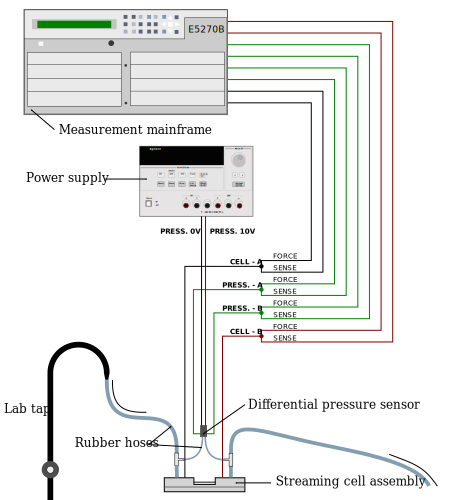
\includegraphics{content/pt1/01-PowerHarvesting/graphics/measurementSetup}
        \caption{\label{fig:measurementSetup}Diagram showing the measurement setup used to measure power output from streaming cell energy harvesters.}
    \end{figure}

    \begin{table}
        \centering
        \begin{tabular}{r|l}
        CELL - A & Voltage/current at high-pressure side of cell\\
        PRESS. - A & Output A of pressure sensor\\
        PRESS. - B & Output B of pressure sensor\\
        CELL - B & Voltage/current at low-pressure side of cell
        \end{tabular}
        \caption{\label{tab:measurementSetup_legend}Definitions for labels used in \ref{fig:measurementSetup}}
    \end{table}


  \subsection{Measurement issues}


    There are two issues with the measurement setup that may impact the measurements.
    Firstly, the electrodes used were copper and are susceptible to polarisation by electrolysis.
    Secondly, the differential pressure sensor is only rated to 15\thinspace PSI (approximately \SI{100}{\kilo\pascal}), less than half the maximum pressure developed across the cell.

    Electrolysis on at the electrode surface causes the electrodes to polarise.
    This results in a semi-permanent offset voltage appearing between the electrodes.
    That offset voltage is opposite in polarity to what is developed while cell is in operation.
    By reversing the flow of water through the cell the polarisation can be reversed.
    Use of more suitable electrode materials would reduce this effect, for instance platinum black electrodes.
    Copper was used for the electrodes as it was cheap, easily obtainable, and easy to work with.
    Offset voltages can be removed after measurement by subtraction.
    Obviously this is not a perfect solution but will be sufficient as the offset itself can be measured so it will be well known.

    From measurement of the output \emph{voltage} of the cells, the presented graphs and figures have been adjusted to remove the effects of electrolysis.
    This was done by adding an offset to the measured data to shift the y-intercept up to \SI{0}{\volt}.
    This provides a more accurate representation of the situation had platinum black electrodes been used.
    As no absolute data is taken from these measurements, the y-intercept adjustment does not affect any subsequent predictions made about the cells.
    Only the gradient of the output, relative to the pressure applied is used; and even then, only to select a suitable candidate cell for power measurement.
    \emph{Most importantly}, no offsets have been applied to measurements of the cell power output.

    Although the maximum rated pressure of sensor was 15\thinspace PSI (approximately \SI{100}{\kilo\pascal}), the sensor's output remained linear up to our maximum pressure of 40\thinspace PSI (\SI{275}{\kilo\pascal}).
    I expect that exceeding the sensors specified pressure will result in a lower `mean time to failure', but its output remained true.
    As a precaution, a tyre pressure gauge was used to roughly confirm the output of the sensor at the end of the cell measurements.
    This was a crude test, however it's output matched that of the differential pressure sensor, so was taken as a good indication of its accuracy.


\section{Results}
  \label{sect:part1_energyHarvesting_results}


  Results from streaming cell measurement are broken into two sub-sections.
  The first presents the output voltage of the ten cells in response to applied water pressure.
  From these measurements, the cell with the highest voltage/pressure ratio is found.
  The second sub-section shows the maximum power that can be harvested from that cell.
  These are the most important measurements as they reveal the energy conversion efficiency of the cells.


  \subsection{Streaming voltage versus pressure}



    \Cref{fig:streamingCell_all_adjusted} shows adjusted results of streaming voltage measurements from each of the ten cells.
    A full set of figures, one cell per graph, can be found in \cref{appendix:streamingCellMeasurements} as \Crefrange{fig:VvsP_26um}{fig:VvsP_245um}.
    It represents the first successful measurements I had made of streaming cells.
    During these measurements three cells burst under pressure; two were dropped and subsequently shattered; and one suffered epoxy failure, loosing its acrylic base plate.
    No measurements of flow rate or output current were made during these early experiments.
    As a result they reveal very little about the efficiency of the cells themselves.
    We cannot determine either the mechanical energy put into the cells, nor the output power available.
    However, we can relate these measurements to those made by Gu and Li; as will be shown and discussed shortly.

    \begin{figure}
        \centering
        \includegraphics{content/pt1/01-PowerHarvesting/graphics/graph_streamingVoltageGradient_vs_height}
        \caption{\label{fig:streamingCell_all_adjusted}Plot showing adjusted streaming voltages versus applied pressure.}
    \end{figure}

    \begin{figure}
        \centering
        \includegraphics{content/pt1/01-PowerHarvesting/graphics/streamingCell_slopeVsChannelHeight}
        \caption{\label{fig:streamingCell_scatter_voltGradVsHeight}Scatter plot of voltage/pressure gradient versus channel height for each of the measured channels.}
    \end{figure}

    \begin{figure}
        \centering
        \includegraphics{content/pt1/01-PowerHarvesting/graphics/graph_streamingVoltageGradient_vs_height_noCorrection}
        \caption{\label{fig:streamingCell_all_unadjusted}Plot showing un-adjusted streaming voltages versus applied pressure.}
    \end{figure}

    The cell having an internal height of \SI{56}{\micro\meter} required an offset adjustment of \SI{405}{\milli\volt} to remove its vertical offset.
    This indicates that the electrodes were highly polarised by the time measurements were made.
    This effect is especially evident in \cref{fig:streamingCell_all_unadjusted}, which shows raw measured data without vertical offset adjustment.
    Some of the traces exhibit a certain amount of `jitter' in their pressure-to-voltage gradients.
    This is likely due to the time difference between adjacent measurement points.
    Measurement points were not taken monotonically, instead being extracted from a number of pressure cycles.

    \Cref{fig:streamingCell_scatter_voltGradVsHeight} shows the streaming voltage to pressure gradients versus channel height.
    This data has been taken from the previous graph (\cref{fig:streamingCell_all_adjusted})) to show the response as a function of channel height.

    % Edit checkpoint 2015-09-13 19:43


  \subsection{Output power versus load resistance}


    \begin{figure}
        \centering
        \includegraphics{content/pt1/01-PowerHarvesting/graphics/graph_streamingCell_outputPower_resistanceSweep}
        \caption{\label{fig:streamingCell_maxPower}Graph showing output power versus effective load resistance for a \SI{71}{\micro\metre} high channel at a pressure of \SI{260}{\kilo\pascal}.}
    \end{figure}

    \Cref{fig:streamingCell_maxPower} shows the characteristic power curve of the \SI{71}{\micro\meter} high streaming cell channel.
    Pressure fluctuations near the end of the experiment are due to usage of the departments water system.
    Their effect is visible in both the streaming voltage and output power traces, highlighting the strong coupling to applied pressure.

    The maximum power delivered by the cell was \SI{1.52}{\nano\watt}, corresponding to a current draw of \SI{33.5}{\nano\ampere} with a streaming voltage of \SI{182}{\milli\volt}.
    Generating this power required \SI{260}{\kilo\pascal} of pressure, resulting in a flow rate of \SI{2.05}{\milli\litre\per\second}.
    This equates to \SI{539}{\milli\watt} of pumping power lost to the device and therefore an energy conversion efficiency of \SI{0.28}{\micro\percent}.


\section{Discussion}
  \label{sect:part1_energyHarvesting_discussion}


  Initial measurements of streaming voltage revealed that the output voltage is directly proportional to applied pressure.
  Containing pressures reaching \SI{260}{\kilo\pascal} within glass structures is difficult.

  Comparing the streaming voltage measurements taken from each of the ten cells to the measurements made by Gu and Li yielded surprising results.
  In their paper~\cite{Gu2000}, they determined the zeta potential ($\zeta$) and surface conductivity ($\lambda$) by plotting measurements and fitting a linear equation to their data.
  The use the y-intercept of the resulting line to give the inverse zeta potential and the slope of the line gave information about the surface conductivity.

  \begin{figure}
      \centering
      \includegraphics{content/pt1/01-PowerHarvesting/graphics/GuLi_DIUF}
      \caption{\label{fig:Gu_Li_comparison_DUIF}Plot showing measured data from Gu and Li's paper on streaming cells relating the streaming voltage and pressure differential to the channel height with distilled water as the working fluid}
  \end{figure}

  \begin{figure}
      \centering
      \includegraphics{content/pt1/01-PowerHarvesting/graphics/GuLi_NaCl}
      \caption{\label{fig:Gu_Li_comparison_NaCl}Plot showing measured data from Gu and Li's paper on streaming cells relating the streaming voltage and pressure differential to the channel height with a \SI{1}{\milli\mole} sodium chloride solution as the working fluid}
  \end{figure}

  Their results for three streaming cells are shown here (taken from \cite{Gu2000}) as \cref{fig:Gu_Li_comparison_DUIF,fig:Gu_Li_comparison_NaCl}.
  The first (\cref{fig:Gu_Li_comparison_DUIF}) shows measurements when distilled water is used as the working fluid; the second (\cref{fig:Gu_Li_comparison_NaCl}) shows the measurements for a weak saline solution.
  It is interesting to note that they have what looks to be fairly linear data, although it is hard to tell with only three channel sizes.

  \begin{figure}
      \centering
      \includegraphics{content/pt1/01-PowerHarvesting/graphics/graph_streamingComparison_gu}
      \caption{\label{fig:streamingCell_scatter_Gu_Li}Scatter plot with results of streaming cell measurements in terms of those made by Gu and Li~\cite{Gu2000} (for comparison).}
  \end{figure}

  By comparison, \cref{fig:streamingCell_scatter_Gu_Li} plots the same variables from measurements taken from the ten streaming cells fabricated here.
  In this graph $\lambda_{b}$ has been replaced with $\sigma$, where both refer to the bulk conductivity of the solution; and $E_{s}$ has been replaced with $V_{s}$, were both refer to the streaming potential.
  The response to variation of channel height is clearly non-linear.
  Their method of finding the zeta potential rests on the following rearrangement:
  \begin{eqnarray}
      \frac{\varepsilon_{r}\varepsilon_{0}\Delta P}{\mu V_{s}\sigma} = \frac{1}{\zeta} + \left( \frac{2\,\lambda}{\zeta \sigma}\right)\,\frac{1}{\delta}
  \end{eqnarray}
  where $\lambda$ is the surface conductivity and $\delta$ is the channel height.
  So as the channel height ($\delta$) tends to infinity, the left hand side tends toward the zeta potential ($\zeta$).
  This notion seems counter intuitive since the zeta potential is defined at the plane of sheer (as shown in \cref{fig:doubleLayer_anatomy}), relative to the solution bulk.
  The equation is stating that no-matter how far you separate the walls, the minimum voltage-pressure gradient you can get is still set by the zeta potential.

  Measurement of the output power generated by the \SI{71}{\micro\meter} streaming cell is promising.
  From this measurement the power transfer curve is evident.
  Referring back to the model presented as \cref{fig:StreamingCell_Schematic-representation}, we can now calculate the channels internal electrical resistance ($R_{cell}$).
  We know from the graph that the maximum power transfer occurred at a current of \SI{33.5}{\nano\ampere} with a streaming voltage of \SI{182}{\milli\volt}.
  Via Ohm's law this equates to a load resistance ($R_{out}$) of \SI{5.43}{\mega\ohm}, which from the maximum power theorem we know must be equal to the cells internal resistance.


\section{Concluding Remarks}
  \label{sect:part1_energyHarvesting_conclusion}

  Conversion of mechanical pumping into electrical energy can be done with narrowly separated plates of glass.
  The conversion efficiency seen here was low, much lower than reported in the literature.
  A channel \SI{1}{\centi\meter} by \SI{3}{\centi\meter} by \SI{71}{\micro\meter} produced \SI{1.5}{\nano\watt} under a pressure differential of \SI{260}{\kilo\pascal}.
  That took \SI{359}{\milli\watt} of pumping power to produce, yielding an efficiency in the order of \SI{0.1}{\micro\percent}.
  Precision engineering, with regards to cell construction, will likely lead to greater efficiency.
  This is based on reports from the literature, where higher efficiency channels utilised much narrower channels.

  Measurements of ten streaming cells were compared to the results published by Gu and Li.
  The linear relationship of Gu and Li between channel height and their plotted parameter could not be reproduced.
  Instead, results showed a highly non-linear relationship as shown in~\cref{fig:streamingCell_scatter_Gu_Li}.
  The gradient of measurement points within the range of channel heights measured by Gu and Li is reversed.
  The reason for the discrepancy is not clear.

  The streaming voltage was found to scale linearly with the applied pressure.
  This could potentially be useful as a means of sensing water flow rates.
  A dual purpose such as power sourcing and flow measurement lends itself well to water metering applications.


  % Edit checkpoint 2015-09-13 19:49


   \chapter{Applicability to Water Metering}
     \label{chap:part1_waterMetering}
     %!TEX root = ../../../thesis.tex
\section{Current Trends in Water Metering}
  Automatic meter reading systems offer advantages to suppliers of town water.
  These include increased billing frequency, remove the need to access the consumers' property~\cite{Chang2012}, and help reduce overall water consumption.
  Another factor in the adoption automatic meter reading technologies is the ability to detect water leaks.
  It has been estimated that as much as \SI{10}{\percent} of post-meter water consumption is due to leakage in the residential sector.
  A study by Britton et al.\ found that by communicating with those customers whose water supply exhibited signs of leakages, a total reduction of  \SI{89}{\percent} of night-time flow rates was achieved.
  This is in contrast to a control group whose night-time usage increased by over \SI{50}{\percent}.
  In areas where water availability is limited, conserving water is an important issue.
  The benefits of automatic water metering are not only geared toward fair pricing but detecting and monitoring the network as a whole.

  \begin{figure}
    \centering
    \includegraphics[width=0.9\textwidth]{content/pt1/02-WirelessWaterMeter/graphics/meter}
    \caption{\label{fig:Photo_DomesticWaterMeter}Photograph of a domestic water meter (Kent PSMT 25mm) typically found in the Auckland region.}
  \end{figure}

  Domestic water meters are typically placed at a property's boundary in a plastic box set into the ground.
  The meter at my Auckland home is shown as \cref{fig:Photo_DomesticWaterMeter}.
  This is a typical meter for the Auckland region, which has been installed approximately eight meters into our property from the road-side.
  Due to their location, it is usually not feasible to wire them to an electrical grid.
  No commercially viable domestic energy harvesting water meters, suitable for burial, exist on the market as of writing.

  \begin{figure}
    \centering
    \includegraphics[width=0.5\textwidth]{content/pt1/02-WirelessWaterMeter/graphics/hydro-WMBUSWLESSM}
    \caption{\label{fig:Photo_waterwareMeter}Photograph of the a wireless transmitting module from Waterware NZ. The device clips onto a compatable water meter and contains its own battery~\cite{BMeters2014}.}
  \end{figure}

  A common configuration for wireless automatic meter reading is to have a reader/transmitter device that is separate to the meter itself.
  This allows new businesses to enter the remote metering market without having to develop metering technologies.
  Such a device may sit on the meter's display or have a wire that connects it to the meter.
  The design; being a simple tamper-proof, clip-on device; means that it must be powered by batteries.

  Current automatic meter reading systems employ long-life, non-rechargeable batteries.
  These meter reading systems have a battery life of around ten years~\cite{BMeters2014}, which is near the shelf-life of the battery itself.
  We want to see if streaming cells could be used as a means to provide sufficient energy to monitor water usage.
  If possible, a suitable harvester would remove the need for batteries, but require plumbing into the domestic feed.
  The resulting device would not be an attachment, but a replacement for the traditional water meter.
  This would mean that it would have to take on the role of metering water usage.


\section{Appropriateness of Streaming Cell Harvesters}

  In \cref{chap:harvestingEnergy} we discussed electric power generation from streaming cells.
  I demonstrated a \SI{0.2}{\micro\percent} conversion efficency from water flow and pressure.
  I also found the streaming voltage is directly proportional to the pressure across a cell.
  Can that pressure dependence give a way to meter water consumption while generating power? Probably.
  But that sort of question is only relevant if the harvester is feasible.

  To find that out - we need to know how much energy is available to an energy harvester.


  \subsection{Readily harvestable energy}
    This section determines the amount of enery available to an energy harvester.
    The harvester envisioned is intended for domestic water metering so we start by building a profile of domestic water consumption.
    Then by finding how much energy is lost inside a typical water meter we will know how much energy a harvester has available.

    \begin{table}
      \centering
      \begin{tabular}{r l|r|r|l}
        Item & Measurement & Summer & Winter & Unit\\
        \hline\hline
        \multirow{4}{*}{Shower} & Duration & 6.6 & 7.0 & minutes\\
                                & Volume & 50.0 & 52.5 & litres\\
                                & Flow & 8.1 & 8.0 & litres/minute\\
                                & Frequency & 0.9 & 0.9 & /person/day\\
        \hline
        \multirow{2}{*}{Washing}& Volume & 122 & 123 & litres\\
                                & Frequency & 0.35 & 0.36 & /person/day\\
        \hline
        \multirow{2}{*}{Toilet} & Volume & 6.6 & 6.8 & litres\\
                                & Frequency & 4.9 & 4.5 & /person/day\\
      \end{tabular}
      \caption{\label{tab:consumption_figures}Summary of characteristics for typical toilet usage, data taken from~\cite{Heinrich2008}.}
    \end{table}

    In 2008, Heinrich monitors water consumption of 51 homes throughout Auckland in 2008~\cite{Heinrich2008}.
    The report shows that the majority of domestic water is consumed by the shower (\SI{30}{\percent}), washing machine (\SI{27}{\percent}) and toilet (\SI{20}{\percent}).
    Together these account for over \SI{75}{\percent} of domestic water consumption.
    Data shown in \cref{tab:consumption_figures} was taken from that report in order to build a typical water usage profile.
    In 2007, Heinrich published a similar report which also contained water flow profiles~\cite{Heinrich2007} for each of the three items considered.

    \begin{figure}
      \centering
      \includegraphics[width=\linewidth]{content/pt1/02-WirelessWaterMeter/graphics/graph_profile}
      \caption{Sample profile showing constructed instances of washing machine use, a shower and a toilet flush.
      Washing machine usage is broken into two parts corresponding to a wash and rinse cycle.}
      \label{fig:profileSample}
    \end{figure}

    Data from those reports has been used to build a domestic water usage profile.
    \Cref{fig:profileSample} shows the flow rates for each of the items
    The profile fits the usage statistics of a home with two occupants according to the previously mentioned reports over the duration of a week.

    During that time five uses of a washing machine, fourteen showers and fifty six toilet flushes occur.
    \Cref{fig:profileSample} shows
    A sample of the usage profiles of each item is shown in Fig. \ref{fig:profileSample}.

    \begin{figure}
        \centering
        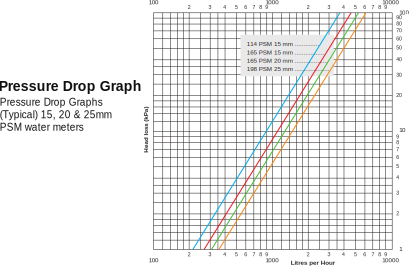
\includegraphics[width=\linewidth]{content/pt1/02-WirelessWaterMeter/graphics/Kent-PSM-HeadLoss}
        \caption{Graph showing the pressure developed across the Kent PSM series mechanical water meters. Taken from~\cite{Elster2008}.}
        \label{fig:headloss}
    \end{figure}

    \begin{figure}
        \centering
        \includegraphics[width=\linewidth]{content/pt1/02-WirelessWaterMeter/graphics/graph_pressureLoss}
        \caption{Graph showing fitted curve to the pressure loss graph presented as \cref{fig:headloss}.}
        \label{fig:headloss_fit}
    \end{figure}

    \begin{figure}
        \centering
        \includegraphics[width=\linewidth]{content/pt1/02-WirelessWaterMeter/graphics/graph_harvest}
        \caption{Calculated power dissipation by a typical domestic mechanical water meter for each of the sample profile events.}
        \label{fig:powerDissipated_meter}
    \end{figure}

    Fig.~\ref{fig:headloss} shows the pressure head loss curve from a water meter typically installed at New Zealand homes (Kent PSMT 25mm)~\cite{WatercareNewZealand2014}.

    Using this curve we calculate power dissipation in a water meter during a washing machine cycle, shower, and toilet flush; presented as \cref{fig:powerDissipated_meter}.
    The total energy dissipated within the meter for each events is:
    \begin{itemize}
    \item \SI{547}{\joule} per load of washing,
    \item \SI{222}{\joule} per shower, and
    \item \SI{24.3}{\joule} per flush of the toilet.
    \end{itemize}

% washing machine volume = 122.00 l
% shower volume = 49.50 l
% toilet volume = 6.22 l
% washing machine energy = 172.08 l
% shower energy = 72.62 l
% toilet energy = 5.07 l

    % These figures are based on average duration and flow rates as found in \cite{Heinrich2008}, and the estimated head loss from Fig.~\ref{fig:headloss}.
    Over an average week the reference water meter would dissipate approximately \SI{7.20}{\kilo\joule} of energy; averaging \SI{1.03}{\kilo\joule} per day.


  \subsection{Domestic harvester design}



    \begin{figure}
      \centering
      \includegraphics[width=0.9\textwidth]{content/pt1/02-WirelessWaterMeter/graphics/harvester}
      \caption{\label{fig:Diagram_harvester}Diagram showing the intended design of streaming cell harvester suitable for domestic connection.}
    \end{figure}

   \chapter{Energy Requirements for Electronic Metering}
     \label{chap:part1_energyHarvestingRequirements}
     %!TEX root = ../../../thesis.tex

The amount of energy lost in a mechanical water meter has been estimated, as has the fraction of that energy which can be harnessed.
Now, the amount of energy required to operate an electronic water meter is sought.
This estimation will reveal how much further the cells built earlier would need to be improved to be viable.

\section{Microcontrollers}

  Central to the operation of an electronic water meter is the microcontroller (MCU).
  The primary function of the microcontroller is to read and log the amount of water consumed by the meter.
  The programme contained on the controller will also decide when to transmit that data and monitor energy usage.
  It is therefore a key component and is expected to consume the majority of energy.

  This chapter compares the power consumption and operational efficiencies of six low power MCUs deemed suitable for use in electronic metering applications.
  These microprocessors are low power, general purpose, 8-bit processors from Microchip, Atmel, and Freescale.
  Each of the microprocessors will have their energy consumption recorded while carrying out various functions over a range of supply voltages.
  Such measured functions are analogue-to-digital conversion, non-volatile memory writes, processing, and sleeping.


  \subsection{Selection of low power processors}

    \begin{sidewaystable}
      \begin{centering}
        \begin{tabular}{|l|l|l|l|l|l|l|l|}
        \cline{2-8}
        \multicolumn{1}{l|}{} & PIC16F1827  & PIC16F887  & PIC16F688  & PIC12F675  & ATtiny25V  & ATtiny13V  & MC9S08QG8 \tabularnewline
        \hline
        Vdd (min)  & 1.8  & 2.0  & 2.0V  & 2.0  & 1.8  & 1.8  & 1.8 \tabularnewline
        Vdd (max)  & 5.5  & 5.5  & 5.5V  & 5.5  & 5.5  & 5.5  & 3.6 \tabularnewline
        I (sleep)  & 30nA  & 50nA  & 50nA  & 1nA  & 100nA & <100nA & 450nA\tabularnewline
        CLOCK (min)  & 31kHz  & 31kHz & 31kHz & 31kHz & 16kHz & 16kHz & 1MHz \tabularnewline
        CLOCK (max)  & 32MHz  & 8MHz  & 8MHz  & 4MHz  & 16MHz & 9MHz  & 10MHz\tabularnewline
        EEPROM  & 256B  & 256B  & 256B  & 128B  & 128B  & 64B  & \dag{}\tabularnewline
        Serial  & USI  & USI  & USI  & --  & USI  & --  & USI \tabularnewline
        USART  & UART  & UART  & UART  & --  & --  & --  & -- \tabularnewline
        ADC  & 10bit  & 10bit & 10it  & 10bit & 10bit & 10bit & 10bit\tabularnewline
        \hline
        \end{tabular}
      \end{centering}

      \begin{centering}
      \dag Has 8,192 bytes of software programmable flash (16 pages of 512 bytes each).
      \end{centering}

      \begin{centering}
      \ddag Has 256 bytes of software programmable flash (4 pages of 64 bytes each).
      \end{centering}

      \caption{\label{tab:MCUfeaturecomparison} Feature comparison of benchmarked microprocessors.}
    \end{sidewaystable}

    The following processors were chosen from the three chosen manufacturers.
    \begin{itemize}
    \item Microchip PIC16F1827
    \item Microchip PIC16F688
    \item Microchip PIC12F675
    \item Atmel ATtiny25V
    \item Atmel ATtiny13V
    \item Freescale MC9S08QG8
    \end{itemize}
    A basic feature comparison of the MCU selection is shown in table \ref{tab:MCUfeaturecomparison}.





% \section{Power consumption}

% Each of the MCUs were programmed to carry out various tasks which
% were performed over their specified range of operating voltages and
% operating frequencies. While the chips where carrying out these tasks
% their power consumption was measured by an Agilent E5270B Precision
% Mainframe via a PC and a Tektronix MSO 4054 Oscilloscope for timing
% purposes. Details on how each of the tests where carried out, as well
% as raw data, can be found in appendix %\ref{Appendix:Measurements} .


  \subsection{Benchmarking power consumption}

    It is important to ensure that each processor is operated so as to minimise power consumption, which meant taking certain precautions.
    Spare pins were set as outputs and tied to Vdd with \SI{10}{\kilo\ohm} resistors.
    Unused peripherals were disabled including any watchdog timers and brownout detection circuitry.
    To allow more accurate sleep current measurements, the chips were placed in a chip carrier with \SI{10}{\kilo\ohm} resistors soldered between the general purpose pins and Vdd.
    The chip and carrier was washed in isopropyl alcohol and dried before being suspended by connections to the measurement device.
    This step minimises leakage current between the pins due to oils and dirt that may be transferred by touching or resting on a table.
    Measurements were carried out using the Agilent E5270B Precision Measurement Mainframe.
    This device has been used for most other measurement situations throughout this thesis for its high impedance inputs and measurement accuracy.


    \subsubsection{Sleep mode}


      \begin{figure}
        \centering
        \includegraphics{content/pt1/03-EnergyRequirements/graphics/Graph_All_Sleeping_Current}
        \caption{\label{fig:All_Sleep_Current}Graph showing current consumed by MCUs in sleep mode versus supply voltage.}
      \end{figure}

      A microprocessor in sleep mode is essentially powered off, the difference being that volatile data is preserved.
      In order to consume as little power as possible an MCU should spend as much time in sleep mode as possible.
      The power consumption while sleep states will determine a large part of the water meters overall energy requirements.

      \Cref{fig:All_Sleep_Current} shows the amount of current consumed by each MCUs while in their deepest sleep states.
      Surprisingly, the PIC16F1827 consumes the most current in this state, almost one thousand times more than the specified sleep current of \SI{30}{\nano\ampere}\cite{PIC16F1827}.
      The Freescale MC9S08QG8 consumed energy at an average of 11\% higher than specified \cite{MC9S08QG8}.
      Both the Atmel ATtiny13V and ATtiny25V fell within their specification, \cite{AtmelATtiny13,AtmelATtiny25} respectively.
      The Microchip PIC12F675 fell within specification\cite{PIC12F675} and was clearly ahead in terms of minimum current draw during sleep.

      There appears to be a trade-off between the two Atmel processors in the way of minimum power consumption and minimum response to Vdd.
      The ATtiny13V required approximately 2.7 times less power than the ATtiny25V at 1.8V, but above 2.5V the ATtiny25V is more draws less current.

      As the PIC16F1827 was so far off its specified value, measurements were repeated numerous times using code written in both assembler and HI-TECH C.
      A total of five different processors were tried, all giving the same result.
      All steps outlined in the PIC16F1827's datasheet to reduce power consumption had been followed.


    \subsubsection*{Disclaimer on processing}


      Measuring the amount of power required to process information is complicated.
      The way each chip carries out processing operations internally can differ from one another, even though all produce the same result.

      \begin{table}
        \centering
        \begin{tabular}{r|c}
          & Instructions\\
          \hline
          PIC16F1827 & 53\\
          PIC16F688 & 35 \\
          PIC12F675 & 35 \\
          ATtiny25V & 120 \\
          ATtiny13V & 120 \\
          MC9S08QG8 & 145
        \end{tabular}
        \caption{\label{tab:Number-of-instructions}Instruction-set size for each tested microprocessor.}
      \end{table}


      \begin{algorithm}
        \begin{lstlisting}
        if (danger >= 5) flight();
        else fight();
        \end{lstlisting}
        \caption{\label{alg:Simple-C-code-representation}Simple C-code representation of a branch instruction.}
      \end{algorithm}


      To illustrate, algorithm \ref{alg:Simple-C-code-representation} shows a simplified programme.
      To determine  the programme's outcome the processor must first evaluate whether `danger' is greater than or equal to five.
      Then it will either branch to the function `fight' or continue on to execute the function `flight'.

      \begin{algorithm}
        \begin{lstlisting}
        load 5 into register 001
        load danger into register 002
        branch-if-greater-or-equal 001 002 flight_call
        call-subroutine fight
        jump-to continue
        [flight_call]
        call-subroutine flight
        [continue]
        \end{lstlisting}
        \caption{\label{alg:Psudo-machine-code1}Pseudo machine-code representation
        of a branch instruction.}
      \end{algorithm}

      \begin{algorithm}
        \begin{lstlisting}
        load danger into register 001
        subtract-from-register 001 5
        branch-if-minus 001 fight_call
        call-subroutine flight
        jump-to continue
        [fight_call]
        call-subroutine fight
        [continue]
        \end{lstlisting}
        \caption{\label{alg:Psudo-machine-code2}Pseudo machine-code representation of an alternative branch instruction.}
      \end{algorithm}


      Algorithms \ref{alg:Psudo-machine-code1} and \ref{alg:Psudo-machine-code2} demonstrate two different ways of implementing \ref{alg:Simple-C-code-representation} using pseudo machine-code.
      The decision of which to use is made by the compiler, which \emph{should} take the instructional efficiency of the specific MCU into account.
      This is an overly simplistic example, but it illustrates that there are multiple paths leading to the same result.
      Importantly, not all of those paths require the same amount of effort on the processor's behalf.
      This means that the compiler's ability to optimise code efficiently plays a role in determining the overall performance of the chip.
      This also means that the programmer should not be concerned with instructional efficiency as the compiler should transform C-code into machine code that best suits the target MCU.

      Another factor in processing efficiency comes down to the number of different instructions it is capable of.
      The list of instructions a processor is capable of is called its instruction set.
      Most 8-bit MCUs are based on reduced instruction set computing (RISC) architecture, as opposed to complex instruction set computing (CISC).
      When compared to a CISC based CPU, a RISC based chip is simpler and therefore usually cheaper to produce and simpler to program.
      However, ``Instruction traces from CISC machines consistently show that few of the available instructions are used in most computing environments''\cite{ComputerArch}, meaning that many of the extended operations in CISC designs are underutilised.
      Processors with smaller instruction sets are capable of achieving the more complex operations by chaining multiple instructions together.
      This means that processors with smaller instruction sets may take longer to execute certain instructions.
      Finally, the frequency of a microprocessor isn't necessarily the frequency at which it performs operations, although sometimes it is.
      For instance, the Atmel and Freescale microprocessors perform one instruction per clock cycle, whereas the Microchip processors perform one instruction every four clock cycles.


    \subsubsection{Processing}

      \begin{figure}
        \centering
        \includegraphics{content/pt1/03-EnergyRequirements/graphics/Graph_PIC16F1827_Clock_Power}
        \caption{\label{graph:CLK_POWER_16F1827}Graph showing power consumed by the PIC16F1827 while processing versus supply voltage.}
      \end{figure}

      \begin{figure}
        \centering
        \includegraphics{content/pt1/03-EnergyRequirements/graphics/Graph_PIC16F688_Clock_Power}
        \caption{\label{graph:CLK_POWER_16F688}Graph showing power consumed by the PIC16F688 while processing versus supply voltage.}
      \end{figure}

      \begin{figure}
      \centering
        \includegraphics{content/pt1/03-EnergyRequirements/graphics/Graph_PIC12F675_Clock_Power}
        \caption{\label{graph:CLK_POWER_12F675-1}Graph showing power consumed by the PIC12F675 while processing versus supply voltage.}
      \end{figure}

      \begin{figure}
      \centering
        \includegraphics{content/pt1/03-EnergyRequirements/graphics/Graph_ATtiny25V_Clock_Power}
        \caption{\label{graph:CLK_POWER_ATtiny25V}Graph showing power consumed by the ATtiny25V while processing versus supply voltage.}
      \end{figure}

      \begin{figure}
        \centering
        \includegraphics{content/pt1/03-EnergyRequirements/graphics/Graph_ATtiny13V_Clock_Power}
        \caption{\label{graph:CLK_POWER_ATtiny13V}Graph showing power consumed by the ATtiny13V while processing versus supply voltage.}
      \end{figure}

      \begin{figure}
        \centering
        \includegraphics{content/pt1/03-EnergyRequirements/graphics/Graph_MC9S08QG8_Clock_Power}
        \caption{\label{graph:CLK_POWER_MC9S08QG8}Graph showing power consumed by the MC9S08QG8 while processing versus supply voltage.}
      \end{figure}

      Results in this section are expressed in terms of instructions per second (IPS).
      The Microchip PIC16F1827 displayed the lowest energy usage with \SI{10}{\micro\ampere} while clocking \SI{7.75}{\kilo IPS} (as shown in \cref{graph:CLK_POWER_16F1827}).
      Microchip MCUs complete one instruction every four clock cycles, so the \SI{7.75}{\kilo IPS} actually corresponds to a standard clock frequency of \SI{31}{\kilo\hertz}.

      % Edit checkpoint 2015-09-17 18:59

      \Cref{graph:CLK_POWER_16F688} shows that the PIC16F688 consumes less power than the PIC16F1827 at low voltages for the same instruction rates (except at 7.75kIPS).
      There appears to be a flatter response in power consumption with respect to Vdd in the PIC16F1827.
      Again, this appears to be a similar trade-off to what was mentioned earlier (in \cref{fig:All_Sleep_Current}) with the Atmel chips.

      The PIC12F675 (\cref{graph:CLK_POWER_12F675-1}) used approximately the same power as the PIC16F688 (\cref{graph:CLK_POWER_16F688}) for its \SI{1}{\mega IPS} trace.
      \Cref{graph:CLK_POWER_ATtiny25V,graph:CLK_POWER_ATtiny13V} show both Atmel MCUs having similar requirements.
      The MC9S08QG8, although being able to clock the slowest, performed very poorly at low frequencies.
      At \SI{1.95}{\kilo IPS} it consumed approximately the same amount of power as the Microchip MCUs operating at \SI{1}{\mega IPS}.

      Overall, the PIC16F1827 gives the widest range of power consumption options, with the ATtiny25V offering similar performance options.

    \subsubsection*{Joules of energy consumed per instruction cycle\label{sub:Joules-of-energy}}

      A convenient, and more insightful way to interpret the previous processing power consumption graphs is to calculate the energy spent per instruction performed.
      The energy cost of an instruction cycle can be calculated using equation \ref{eq:JPI calculation}.

      \begin{equation}
      E_{i}=\frac{I\times Vdd}{f_{i}}\label{eq:JPI calculation}
      \end{equation}
      where $E_{i}$ is the number of joules consumed per instruction, $I$ is the current draw, $Vdd$ is the input voltage and $f_{i}$ is the instruction frequency.

      Figure \ref{fig:Per-instruction-cycle} compares the most energy efficient operating conditions of each of the tested chips.
      What is most interesting about this graph is the high degree of overlap.
      Also, the greater efficiencies occur at high operating frequencies.
      A simple rule of thumb for selecting the most power efficient operating frequency based on these results is to choose the highest frequency where the MCU can operate over its full input voltage (Vdd) range.
      For comparison, figure \ref{fig:Per-instruction-ATtiny13V} shows the trade-off made when selecting a higher frequency, which is typical across the range of MCUs tested.

      \begin{figure}
      \begin{centering}
      \includegraphics{content/pt1/03-EnergyRequirements/graphics/Graph_All_Clock_JPI}
      \par\end{centering}

      \protect\caption{\label{fig:Per-instruction-cycle}Graph showing instruction cycle energy consumption for each MCU versus supply voltage.}
      \end{figure}
      \begin{figure}
      \begin{centering}
      \includegraphics{content/pt1/03-EnergyRequirements/graphics/Graph_ATtiny13V_Clock_JPI}
      \par\end{centering}

      \protect\caption{\label{fig:Per-instruction-ATtiny13V}Graph showing instruction cycle energy consumption of the ATtiny13V versus supply voltage.}
      \end{figure}



    \subsubsection{Instruction efficiency}

      \begin{algorithm}
        \begin{lstlisting}
          unsigned short lfsr = 0xACE1u;
          unsigned period = 0;
          do {
            lfsr = (lfsr >> 1) ^ (-(lfsr & 1u) & 0xB400u);
            ++period;
          } while(lfsr != 0xACE1u);
        \end{lstlisting}
        \caption{\label{alg:Benchmarking-algorithm}Benchmarking algorithm}
      \end{algorithm}

      Calculating the amount of energy consumed per instruction only shows part of processor efficiency.
      The amount of processing done per instruction is not taken into account in such measurements.
      Some MCUs have extra instructions that are designed to help speed up code execution by combining commonly used groups of instructions.
      To shed light on instructional efficiency, the number of instructions each of the processors takes to complete a benchmark function is found.
      This will allow for a more accurate representation of execution efficiency.
      The function used to benchmark each of the processors is a linear feedback shift register based pseudo-random number generator \cite{Wikipedia2015}.
      It is well suited to an 8-bit microprocessor as it requires no complex math functions, uses little memory and has a well defined end.
      The code for this function is shown as \cref{alg:Benchmarking-algorithm}.
      It starts with a 16-bit number and runs it through the linear feedback register in a tight loop until the initial value of the 16-bit feedback register is produced again.
      This function steps through every possible combination of bits possible in a 16-bit number (except for 0 and 65535) in a pseudo-random order before exiting the loop.
      The function combines the exclusive-OR (XOR), bit shifting, bitwise AND, increment a value and numerical comparison operations in a tight loop.
      The benchmarking function was compiled and run on each of the MCUs operating at a range of supported frequencies.

      \begin{figure}
          \begin{centering}
              \includegraphics{content/pt1/03-EnergyRequirements/graphics/Graph_All_Clock_Benchmark}
          \end{centering}
          \protect\caption{\label{fig:GraphBar_All_Benchmark}Graph showing the number of instruction cycles taken to complete a benchmark routine for each MCU.}
      \end{figure}

      To determine the instructional efficiency, the code was set to toggle the state of a digital output pin.
      The toggle frequency of that pin was recorded using a Tektronix MSO 4054 oscilloscope.
      The number of instruction cycles each chip took to complete the benchmark was deduced by multiplying the time taken to complete the benchmark by the instruction cycle frequency.
      The results of the benchmark are shown in \cref{fig:GraphBar_All_Benchmark}.
      To calculate the number of instruction cycles taken by the Microchip family of processors, one quarter of the chip's operation frequency was used.
      This meant that the number of clock cycles consumed was four times higher.
      It is clear from \cref{fig:GraphBar_All_Benchmark} that the Atmel (ATtiny25V and ATtiny13V) microprocessors are by far the most efficient microprocessor in terms of executing code using a minimum number of instructions of the selection.
      The reason for this is most probably due to the larger instruction set and higher compiler optimisation.



    \subsubsection{Non-volatile memory}

      In order for a microprocessor to keep information about its current state and recorded data in the event of power loss it must write to non-volatile memory.
      Non-volatile memory is implemented as either electrically erasable and programmable read only memory (EEPROM) or Flash memory.
      Flash memory is similar to EEPROM with the exception that it must be erased in large blocks, or pages, before it can be written to.
      All of the tested MCUs have on-board EEPROM with the exception of the MC9S08QG8 which has flash memory instead.
      Table \ref{tab:MCUfeaturecomparison} shows the amount of non-volatile memory space available on each of the chips.

      \begin{figure}
        \centering
        \includegraphics{content/pt1/03-EnergyRequirements/graphics/Graph_All_EEPROM_JPO}
        \caption{\label{fig:Energy-consumed-EEPROM}Graph showing energy consumed per non-volatile erase/write operation versus MCU supply voltage.}
      \end{figure}

      The energy consumption of each of the chips with EEPROM memory during a 1-byte write operation is shown as \cref{fig:Energy-consumed-EEPROM}.
      A curious situation arose with the PIC12F675 where its calculated energy consumption was negative when operated below \SI{4.7}{\volt}.
      It consumed \emph{less} current while performing write operations than running through the same code loop without performing writes.
      The measurement was repeated several times and produced the same result.
      Those data points were excluded from the plot as they do not represent the true energy cost of writing to EEPROM.
      It is likely that while writing to EEPROM other parts of this chip are disabled or put to sleep.

      In the case of the MC9S08QG8, which has Flash memory instead of EEPROM, the power consumption in the `E + W' trace was calculated as $1/512^{th}$ of consumed page erase energy consumption added to the energy cost of a single write operation.
      The trace labelled `W' (magenta) shows the energy cost for a single write operation.
      In order for the MC9S08QG8 to perform a write operation, the destination byte must have already been pre-erased at an earlier point in time.
      This may be useful for power harvesting since the energy expensive page erase operation, which consumes an average of \SI{302}{\micro\joule}, can be performed when available energy is plentiful.
      These results show that the Microchip and Freescale microprocessors are the most energy efficient when writing to non-volatile memory.



    \subsubsection{Analog-to-digital conversion}

      The operation of an electronic water meter may require that analogue-to-digital conversions are made.
      Measuring the amount of energy consumed per conversion was done in much the same way as the previous tests.
      Each of the chips had similar converters feature-wise.
      Results from the measurements are presented as \cref{fig:Energy-consumed-ADC}.

      \begin{figure}
        \centering
        \includegraphics{content/pt1/03-EnergyRequirements/graphics/Graph_ALL_ADC_JPM}
        \caption{\label{fig:Energy-consumed-ADC}Graph showing the energy consumed per ADC measurement versus MCU supply voltage.}
      \end{figure}


  \section{Wireless Transmission}

    Because water meters are typically installed in remote areas where grid connection is unavailable, data must be collected via wireless interface.
    In Hamilton, a major utility provider has established a wireless mesh network between smart electricity meters installed in residential homes.
    That network utilises ZigBee wireless transceivers, making ZigBee an convenient choice for transmitting water metering data \cite{MalcolmSouness-WELNetworks2012}.
    Two types of wireless transmitters were chosen for energy measurement, a HOPE RF RFM12B transceiver and a Digi International Xbee Series 2 transceiver.
    The power consumption versus time during a wake, send one hundred and sixty bytes, and power down cycle was captured for both transceivers.
    By integrating the area under this curve the total energy consumed per transmission is found.
    The transmitters were kept \SI{1}{\meter} from their receivers with no obstructions between them.
    This represents ideal transmission conditions, something that our electronic water meter is very unlikely to encounter.
    The actual RF reception between a base station and installed meter will vary greatly between installations and weather conditions.
    For example, wet ground is likely to obstruct RF transmission due to the transmitter being shielded by a more conductive medium.
    Instead of trying to quantify the energy required in those situations, the best case was measured and an estimate of the worst case is estimated to be one hundred times larger.
    The transmit power can increase by a factor of 320 for the RFM module, however the transmit power only represents a proportion of total power usage.
    The modules must power up, start their internal oscillators, receive the data to be transmitted from the main processor and then transmit the data packets.
    I have crudely estimated that the difference between the lowest and the highest total power consumption, based on reception alone, will be a factor of 100.

    \begin{figure}
      \centering
      \includegraphics{content/pt1/03-EnergyRequirements/graphics/Graph_RFMPower.pdf}
      \caption{\label{fig:Energy-consumed-RFM12B}Graph of power draw from a HopeRF RFM12B transceiver module versus time during a power-up and transmit sequence.}
    \end{figure}

    \begin{figure}
      \centering
      \includegraphics{content/pt1/03-EnergyRequirements/graphics/Graph_XbeePower.pdf}
      \caption{\label{fig:Energy-consumed-XBee}Graph of power draw from a Digi International Xbee Series 2 transceiver module versus time during a wake \& transmit sequence.}
    \end{figure}

    The RFM12B was operated at 433MHz, a frequency that is expected to increase the transmission through walls and soil.
    It has a maximum output power of \SI{5}{\decibel m} (\SI{3.2}{\milli\watt}) at this frequency.
    The Xbee has a maximum output power of \SI{0}{\decibel m} (\SI{1}{\milli\watt}) and operates at \SI{2.4}{\giga\hertz}.
    \Cref{fig:Energy-consumed-RFM12B,fig:Energy-consumed-XBee} show the captured power consumption during the tests.
    The RFM12B used about half as much energy sending the same data as the Xbee.
    Combined with its ability to operate at 433 MHz, the RFM12B is a sensible choice for the electronic water meter.
    In total the RFM consumed \SI{6.71}{\milli\joule} and the Xbee consumed \SI{12.3}{\milli\joule}.
    Adjusting these figures for the worst case (multiplying by one hundred) gives \SI{671}{\milli\joule} for the RFM12B and \SI{1.23}{\joule} for the Xbee.

  \section{Final Estimate of Energy Requirements}

    A crude estimation of an electronic water meter's microprocessor event loop is as follows.
    \begin{enumerate}
      \item Sleep for 1 second
      \item Execute 1000 instructions
      \item Make 2 analogue conversions
      \item Write 2 bytes to non-volatile memory
    \end{enumerate}
    This would allow the microprocessor to watch the display of a mechanical water meter and store the readings.
    This loop would occupy approximately one second, so it will occur 86400 times per day.
    Every so often the collected data would need to be transmitted, a potentially costly exercise in terms of energy usage.
    On top of the previously stated event loop is a data transmission loop which would execute every six hours.
    \begin{enumerate}
      \item Execute 1000000 instructions (Data compression)
      \item Power up and transmit 160 bytes of using RF transceiver
      \item Write 10 bytes to non-volatile memory
    \end{enumerate}

    \begin{table}
      \centering
      \begin{tabular}{|l|l|l|l|}
        \hline
        Mode & Count & Unit & Energy \\ \hline
        Sleep & 1 & seconds & \SI{97.4}{\nano\joule} \\
        Processing & 1000 & instructions & \SI{1.14}{\micro\joule} \\
        ADC & 2 & conversions & \SI{2.56}{\nano\joule} \\
        EEPROM & 2 & bytes & \SI{79.0}{\micro\joule} \\ \hline \hline
        &&Total (per day) & \SI{6.93}{\joule} \\ \hline
      \end{tabular}
      \caption{\label{tab:EnergyBudget-EventLoop} Estimated daily energy expenditure for basic processing functionality}
    \end{table}

    \begin{table}
      \centering
      \begin{tabular}{|l|l|l|l|}
        \hline
        Mode & Count & Unit & Energy \\ \hline
        Processing & 1000000 & instructions & \SI{1.14}{\milli\joule} \\
        Transmit & 160 & bytes & \SI{1.23}{\joule} \\
        EEPROM & 10 & bytes & \SI{394}{\micro\joule} \\ \hline \hline
        &&Total (per day) & \SI{4.93}{\joule} \\ \hline
      \end{tabular}
      \caption{\label{tab:EnergyBudget-Transmission}Estimated daily energy expenditure required to transmit 160 characters every six hours}
    \end{table}

    \Cref{tab:EnergyBudget-EventLoop,tab:EnergyBudget-Transmission} combine the measurements and estimates from the previous sections with the event loop estimation.
    They show that approximately \SI{12}{\joule} would be consumed per day by an electronic water meter.
    It was shown in \cref{sect:part1-WirelessWaterMeter-QuantifyingHarvestableEnergy} that \SI{280}{\joule} of energy is already dissipated in a mechanical water meter per day.
    This equates to a conversion efficiency of \SI{4.28}{\percent}, which would be the minimum efficiency required to run the meter continuously.

    % Edit checkpoint 2015-09-17 19:35

   \chapter{Conclusion}
     \label{chap:part1_conclusion}
     %!TEX root = ../../../thesis.tex

Estimates of energy availability have been made by calculating the amount of energy lost in a traditional water meter.
Those estimates showed that for a typical New Zealand household approximately \SI{280}{\joule} of harvestable energy is available per day.
In the previous section, the amount of energy that would be needed to run an electronic water meter was estimated to be \SI{12}{\joule} per day.
This means that in order to power an electronic water meter a minimum conversion efficiency of \SI{4.28}{\percent} is required.
%However, calculations from cells assembled in \cref{sect:part1_energyHarvesting_measuringStreamingCells} showed that readily obtainable conversion efficiencies are in the order of \SI{0.28}{\micro\percent}.
However, calculations from cells assembled in \cref{sect:part1_energyHarvesting_measuringStreamingCells} showed that readily obtainable conversion efficiencies are in the order of \SI{2.8e-9}.
Conversion efficiencies over \SI{1}{\percent} have not been reported in the literature, and one paper suggests the theoretical maximum is \SI{2}{\percent} \cite{VanderHeyden2006}.
For these reasons, the use of streaming cells as a method of energy harvesting from water and current materials is expected to be infeasible.
The literature suggests there is room for improvement, to levels which would make streaming cell harvesters practical, but these gains are reliant on new nano-materials.

During the course of this research two issues came to light with regards to streaming cell harvesting.
The first issue is a susceptibility to clogging.
Having such narrow openings in a domestic water feed is likely to trap dirt and contaminants at the channel openings.
This lowers the effective efficiency and will require periodic cleaning, lowering the benefit to utility companies.
The second issue is the manufacturing precision required to create the channels.
Parts manufactured with high precision are generally small, but a streaming cell would need precise dimensions and a large surface area.
This could be overcome with the use of materials like porous glass.
As a result of the low measured efficiency, streaming cells for the purpose of energy harvesting are not studied further.
\Cref{part:doubleLayersOnConductors} looks at the electrical impedance of medical implant electrodes.
The research here into double layers and the role they play in energy harvesting applications is directly applicable there.

% Edit checkpoint 2015-09-17 19:38



%% Part 3 - Double layers on conductors
\part{Double Layers on Conductors: Electrical Impedance}
  \label{part:doubleLayersOnConductors}

  For the engineers of medical implant devices, knowing the electrical impedance between electrodes is important.
  Having a tool to simulate such impedances allows those designers to ensure fault free operation of potentially lethal devices.
  A model of the interface impedance between electrode and electrolyte is presented in the proceeding chapter.
  That model was created by my chief supervisor Jonathan Scott and Peter Single of Saluda Medical Sydney.
  Validation of the model was made in a standard solution of saline, but details of how saline concentration affected the parameters were unknown.
  In \cref{part:doubleLayersOnConductors} of thesis thesis I take that model and extend its predictive capability to a range of salinities.
  Having such a model allows for easy comparison between different electrolytes and electrode geometries.
  Using that ability, I characterise the interface in an anaesthetised sheep's spinal cavity and compare the results to the various saline solutions measured in the lab.
  That comparison showed that the situation in live sheep is relatively different to that of standard saline solutions.
  Using the measurement methods developed, I then find a mixture that closely matches the electrical impedance seen in sheep.
  This mixture now serves as an improved test solution for the engineers of medical implant devices.

  \chapter{Interface Modelling In The Electrical Domain}
    \label{chap:theInterfaceModel}
    %!TEX root = ../../../thesis.tex

This chapter looks at each of the components within the interface model.
The parameters that govern the behaviour of those components will be discussed, as will methods of measuring those parameters.
The measurements and determined parameters will be presented in the next chapter (\cref{chap:interfaceParameters}).


\section{The Scott-Single Interface Model}


  \begin{figure}
    \centering
    \includegraphics{content/pt2/07-InterfaceModel/graphics/electrode-electrolyte}
    \caption{\label{fig:electrode-electrolyte}Diagram of two electrodes submerged in an electrolyte solution, which can modelled by the Scott-Single Interface Model.}
  \end{figure}

  \begin{figure}
    \centering
    \includegraphics{content/pt2/07-InterfaceModel/graphics/simpleElectrodeElectrolyteModel}
    \caption{\label{fig:pt2-simpleElectrodeElectrolyteModel}Connection diagram of two electrodes (with interfaces) connected together by the resistivity of an electrolyte solution.}
  \end{figure}
  In 2013, Jonathan Scott and Peter Single published an electrical model of an implantable electrode array in saline\cite{ScottSingle2013}.
  That model simulates the electrical impedance a medical implant device is be subjected to once implanted into a human's spinal cavity.
  It is general enough to use in any situation where electrodes are placed in an electrolyte; a simple case is depicted in \cref{fig:electrode-electrolyte}.
  The model comes in two parts: an electrode interface, and the resistance of the electrolyte between interfaces.
  \Cref{fig:pt2-simpleElectrodeElectrolyteModel} shows the electrical equivalent of connecting two electrodes through an electrolyte.
  It two interfaces, each with the liquid side joined electrically by the resistance of the electrolyte's bulk resistivity.
  The metal side of the interfaces is what the rest of the circuit (such as the implant electronics) connects to.

  \Cref{fig:pt2-interfaceSchematic} shows the electrode-electrolyte interface (the component labelled `Interface' in \cref{fig:pt2-simpleElectrodeElectrolyteModel}.
  It is an electronic equivalent circuit of the transition between the metal of an electrode and the liquid of an electrolyte.
  The interface model that was actually used throughout this thesis is a simplified version of this in that the memristors (elements M\textsubscript{a} and M\textsubscript{b}) have been omitted.
  \begin{figure}
    \centering
    \includegraphics{content/pt2/07-InterfaceModel/graphics/interfaceSchematic}
    \caption{\label{fig:pt2-interfaceSchematic}Electrical schematic of the electrode-electrolyte interface}
  \end{figure}


  \subsection{Inter-electrode resistivity (resistor network)}


    Modelling the resistance between two electrodes in a fixed geometry situation is simply a matter of inserting an appropriately sized resistor between the two interfaces.
    The resistance is dependent on the electrolyte's conductivity, the combined surface area of the two electrodes and the distance between them.
    The St. Jude Medical Octrode is an eight electrode array commonly used in spinal cord stimulator implants.
    Its eight electrodes are made from platinum and are separated along the end of a lead by insulating material.
    An illustration of an Octrode is presented as \cref{fig:StJudeOctrode_Labelled}.
    Modelling such an electrode array requires a resistor network that connects all electrodes to one another.
    To be an adequate representation, the resistance between every possible combination of electrode pairs must match the measured value in an electrolyte.

    \begin{figure}
      \centering
      \includegraphics{content/pt2/07-InterfaceModel/graphics/StJudeOctrodeDiagram}
      \caption{\label{fig:StJudeOctrode_Labelled}St. Jude Medical Octrode. An eight electrode array commonly used in spinal stimulation implants. The electrode numbering shown here will be used throughout this work.}
    \end{figure}

    % Edit checkpoint 2015-09-17 20:23
    \begin{figure}
      \centering
      \includegraphics{content/pt2/07-InterfaceModel/graphics/electrodeRings}
      \caption{\label{fig:electrodeRings}Diagram showing the first three radial volumes expanding from the surface of the electrode and insulating spacer. Each volume has a diameter twice that of the one inside it. These volumes are used mathematically to determine relationship between resistances in the resistor mesh.}
    \end{figure}
    Scott and Single created a resistor network for modelling the electrolyte conductivity based on the geometry of the electrodes and the resistivity of the electrolyte.
    By sectioning the surrounding liquid into cylindrical volumes they calculated the equivalent resistance between those volumes in both radial and longitudinal planes.
    The radii of the volumes double at each layer which correspond to a fixed radial resistance between each layer.
    There are two different radial resistances: one for the rings expanding from the insulating spacers, and one for those expanding from the electrode cylinders.
    The two layers alternate due to each electrode being separated by an insulating spacer.
    \Cref{fig:electrodeRings} illustrates the idea on a subsection of the electrode array by showing three radial volumes surrounding three electrodes and two spacers.
    The longitudinal resistances quarter in size with each ring layer and after the last radial resistor each node is shorted together.
    The full mesh for the eight electrode array is five layers deep with three rows of padding at each terminating end, totalling two hundred and five resistors in total.
    \Cref{fig:pt2-ResistorMesh} shows the resistor network schematic.
    Further details of how the mesh geometry and resistor values were calculated can be found in \cite{Scott2014}.


    The parameters that describe the resistor mesh are:
    \begin{itemize}
    \item $R_{eri}$ - The initial resistance placed radially from an electrode.
    \item $R_{sri}$ - The initial resistance placed radially from a spacer.
    \item $R_{li}$ - The longitudinal resistance.
    \item Depth - Number of layers between the electrode/spacer and the common end node in the ladder
    \item Padding - Number of additional spacing rows to be added to each end of the mesh.
    \end{itemize}

    \begin{figure}
      \centering
      \includegraphics{content/pt2/07-InterfaceModel/graphics/resistorMesh}
      \caption{\label{fig:pt2-ResistorMesh}Resistor mesh used to model the electrical resistance between interface pairs. $R_{li}$ is longitudinal resistance, $R_{sri}$ and $R_{eri}$ is the radial resistance for the spacers and electrodes respectively, and $I$ is an interface.}
    \end{figure}


  \subsection{Interface series resistance (resistor)}


    The series resistor at the right hand side of the model schematic (labelled $R_{S}$) represents the purely resistive component of the interface's impedance.
    As it is in series with all other components in the interface model, there is no way for charge to cross the interface without encountering this resistance.
    The parameter used to denote the interface's series resistance is:
    \begin{itemize}
      \item $R_S$ -- The series resistance of the interface
    \end{itemize}

  \subsection{Polar/double-layer effects (constant phase element)}

    At the centre of the model is the constant phase element (CPE), or fractional pole capacitor.
    A CPE is a device that behaves like a cross between a capacitor and a resistor.
    They are primarily used to describe the capacitance of double layer interfaces, which is the function it serves in this model.
    It is capacitive in the sense that voltage leads current, but by an amount less than \SI{90}{\degree}.
    Mathematically, the \SI{90}{\degree} angle between voltage and current in a capacitor comes from:
    \begin{equation}
    I(t) = C \times \frac{dV(t)}{dt}
    \label{eqn:currentVoltageInCapacitor}
    \end{equation}
    When $V(t)$ is a sine wave, this becomes
    \begin{align}
      I(t) &= C \times \frac{d Sin(t)}{dt}\\
           &= C \times Cos(t)
    \end{align}
    Which describes how the current always \SI{90}{\degree} out of phase with voltage in a capacitor.
    A CPE on the other hand has a phase angle somewhere \emph{between} 0 and \SI{-90}{\degree}.
    This requires a fractional differentiation of \cref{eqn:currentVoltageInCapacitor} such as:
    \begin{equation}
      I(t) = C \frac{d^n V(t)}{dt^n}
    \end{equation}
    where n is a non-integer number.
    Partially applied differential is uncommon outside of pure mathematics.
    % This requires a fractional differentiation of $I(t) = C \times \frac{d^n V(t)}{dt^n}$, something uncommon outside of pure mathematics.
    As a consequence of having a current/voltage relationship of less than \SI{90}{\degree}, a CPE's impedance magnitude decays at a rate lower than 20\ dB/decade.

    SPICE, or any other commonly used circuit simulators, do not support fractional pole capacitors so entering one into the model will require building it up from discrete components.
    \begin{figure}[ht]
      \centering
      \includegraphics{content/pt2/07-InterfaceModel/graphics/Morrison-RC}
      \caption{\label{graph:pt2-morrisonCPE}Ralph Morrison's implementation of a constant phase element using an infinite array of resistor-capacitor pairs (taken from Morrison's paper -- \cite{Morrison1959}).}
    \end{figure}
    In 1959, Morrison demonstrated a way of creating constant phase elements from an infinite array of resistor-capacitor (RC) pairs \cite{Morrison1959}.
    One of Morrison's implementations of a constant phase element is presented as \cref{graph:pt2-morrisonCPE}.
    In that implementation, each parallel branch has precisely chosen resistor and capacitor values such that when summed together the impedance magnitude versus frequency is a constant slope, i.e., the impedance does not flatten at a particular frequency as it would with a single RC pair.
    Creating any element comprised of an infinite number of sub-elements is not possible, however by selecting only those elements that contribute to the bandwidth of interest the result is the same within the selected frequency window.
    Using that method and selecting only RC pairs with a cut-off frequency in the range of \SI{1}{\milli\hertz} to \SI{1}{\mega\hertz}, a practical CPE can be created.

    \begin{figure}
      \centering
      \includegraphics{content/pt2/07-InterfaceModel/graphics/graph_cpe_creation}
      \caption{\label{graph:pt2-cpe_creation}Graph showing how a non \SI{-20}{\decibel} per decade slope can be constructed from a series of \SI{-20}{\decibel} per decade low-pass filters}
    \end{figure}

    \Cref{graph:pt2-cpe_creation} shows the individual contributions from each RC branch in an implementation of a CPE.
    Each grey trace represents a single RC branch within the CPE, as are shown in \cref{graph:pt2-morrisonCPE}.
    The value of the resistor in each branch is evident by the vertical position of the traces, visible at the right-hand side of the graph.
    The branches in this particular example have been spaced in the frequency domain at a density of three per decade, as marked by the black crosses.
    This means that per decade of frequency, there are three corner frequencies, each relating to an RC pair (so three branches for every decade of frequency response).
    Because each of there branches are in parallel, the total response of the CPE as a whole is the superposition of the response of each branch.
    That response is shown as the black trace on the graph.
    The critical observation is that the slope of the resulting trace is different to the slope of the capacitors in each of the individual branches.
    This allows the CPE to behave fractionally as a capacitor, being anywhere between resistive (horizontal response) and capacitive (\SI{20}{\decibel}/decade slope).
    Lines 186--189 of \cref{code:lib_simulate} show how values for the resistors and capacitors within the CPE are calculated.

    The CPE represents readily reversible reactions, polar reorientation, and ionic repulsion and attraction between the electrode's surface and the electrolyte.
    It is capacitive in nature because each of these mechanisms store charge, which can be drawn back by reversing the applied electromotive force.
    Parameters used to describe the behaviour of the CPE are:
    \begin{itemize}
      \item $m$ -- Used to select resistor-capacitor pairs in each branch and ultimately determines the slope of the CPE's frequency response
      \item $k$ -- Spacing of R-C branches with frequency. More branches give a better approximation, at a cost of more branches.
      \item $|Z|$ @ \SI{1}{\kilo\hertz} -- Sets the vertical position of the magnitude of CPE's frequency response at a known frequency
    \end{itemize}

    % Edit checkpoint 2015-09-17 21:17


  \subsection{Faradaic reactions (diodes)}


    If the voltage placed across the interface is kept within certain limits, the CPE and series resistance ($R_{S}$) would be all that is necessary to accurately mimic a single electrode-electrolyte interface.
    But once the electric potential across the interface becomes high enough, Faradaic reactions will occur at the electrode's surface.
    Faradaic reactions are reactions involving charge transfer, adding ionised species to the electrolyte and often producing gas.
    Gas, or any new species, is disastrous in an implanted setting as this causes damage to the implant's host.
    Possible Faradaic reactions between saline and platinum electrodes are:
    \begin{eqnarray}
        Pt + H_{2}O &\Leftrightarrow& PtO + 2 H^{+} + 2 e^{-}\\
        PtO + H_{2}O &\Leftrightarrow& PtO_{2} + 2 H^{+} + 2e^{-}\\
        Pt + H^{+} + e^{-} & \Leftrightarrow & Pt-H\\
        Pt + H_{2}O + e^{-} &\Leftrightarrow& Pt-H+OH^{-}
    \end{eqnarray}

    The electrical current density through an electrode as a function of electrode overpotential and the cathodic and anodic reactions occurring at each electrode is given by:
    \begin{equation}
      i_{net} = i_{0} \left\{ \frac{[O]_{(0,t)}}{[O]_{\infty}}e^{-\alpha_{c}nf\eta} - \frac{[R]_{(0,t)}}{[R]_{\infty}}e^{(1-\alpha_{c})nf\eta}\right\}
      \label{eqn:pt-2_butlerVolmerEquation}
    \end{equation}
    % \Cref{eqn:pt-2_butlerVolmerEquation} describes electrical current density through an electrode as a function of electrode overpotential and the cathodic and anodic reactions occurring at each electrode.
    This is the current-overpotential equation and is derived from the more general Butler-Volmer equation \cite{Merrill2005,ScottSingle2013}.
    In \cref{eqn:pt-2_butlerVolmerEquation}, $i_{net}$ is the net Faradaic current across the electrode-electrolyte interface,
    $i_{0}$ is the exchange current density,
    $[O]_{(0,t)}$ and $[R]_{(0,t)}$ are the oxidant and reductant concentrations at the electrode surface as a function of time,
    $[O]_{\infty}$ and $[R]_{\infty}$ are concentrations of reactant in the bulk electrolyte,
    $\alpha_{c}$ is the cathodic transfer coefficient (approximately 0.5),
    $n$ is the number of moles of electrons per mole of reactant oxidised,
    $f$ is Faraday's constant divided by the product of the gas constant and the absolute temperature ($F/RT$),
    and $\eta$ is the electrode overpotential.
    This equation describes the forward and reverse electrical current through an electrode by separating the forward and reverse reactions: oxidisation and reduction.
    Taking a single half of the equation, either the reduction or oxidisation, yields an equation that is similar to that for the current through a diode; an observation made by McAdams and utilised in the Scott-Single model \cite{McAdams1995}.
    The standard Ebers-Moll equation of a diode equation is:
    \begin{equation}
      I = i_0\left(e^{V_D / n V_T}-1\right) \approx i_0 e^{V_D / n V_T}
      \label{eqn:pt-2_diodeEquation}
    \end{equation}
    where:
    \begin{itemize}
      \item $I$ is the current through the diode,
      \item $i_0$ is the diode saturation current,
      \item $V_D$ is the potential across the diode,
      \item $n$ is the diode's ideality factor, and
      \item $V_T$ is the thermal voltage (defined as the product of Boltzmann's constant and temperature divided by the charge on an electron).
    \end{itemize}
    The two parameters needed to describe the behaviour of the diode are $i_0$ and $n$, which will later be determined for the diodes in the model.
    The diodes themselves can not account for the relative abundance of reactants for the redox reactions ($[O]_{(0,t)}/[O]_{\infty}$ and $[R]_{(0,t)}/[R]_{\infty}$ from \cref{eqn:pt-2_butlerVolmerEquation}), this needs to be considered separately and is discussed next.


  \subsection{Chemical species depletion (memristors)}


    \begin{figure}[ht]
      \centering
      \includegraphics{content/pt2/07-InterfaceModel/graphics/memristorSymbol}
      \caption{\label{fig:pt2-memristorSymbol}Electrical symbol of a memristor, as is used in the original electrode-electrolyte interface model}
    \end{figure}

    A memristor is a two port device that sets its resistance based on its own history.
    The resistance can either depend on the integral over time of the voltage placed across it or the total charge passed through the device \cite{Kvatinsky2012}.
    Its name is a portmanteau of the word `memory' and `resistor' owing to its use of memory to set its resistance~\cite{Williams2008}.

    The memristive device models species depletion in the electrolyte as an increase in resistance in the diode/memristor branch in proportion to the integral of charge passed through the branch.
    As the specific Faradaic reaction proceeds, it consumes the reactants from the electrolyte bulk until eventually none is left.
    Increasing the resistance in series with a conducting diode has the effect of removing that diodes current path from the circuit, simulating the depletion of reactants of the modelled reaction.

    Memristors were removed from the model used in this work as they added complexity that would yield little in the way of research outcomes.
    The diodes are only used to model the \emph{onset} of Faradaic conduction, which is the most relevant parameter of the Faradaic modelling.
    Once these reactions begin, the electrode overpotential has been pushed too far and there is little to be gained from knowing how far the reaction can be run until the reactants have been depleted.
    In an implanted setting it is likely that the electrolyte will circulate throughout the body, bringing new reactants to the electrode's surface over time.
    Species depletion is likely to be a slow process, dependent on the electrolyte volume and species concentration.

    \begin{figure}
      \centering
      \includegraphics{content/pt2/07-InterfaceModel/graphics/interfaceSchematic_noMemristive}
      \caption{\label{fig:pt2-interfaceSchematic_noMemristive}Electrical schematic of the electrode-electrolyte interface without memristors (as used throughout this thesis)}
    \end{figure}

    \Cref{fig:pt2-interfaceSchematic_noMemristive} shows the interface model used throughout the remainder of this thesis.
    Although it is slightly different to the Scott-Single interface model, the other parameters are unaffected by the removal of these elements.

    % Edit checkpoint 2015-09-17 21:31


\section{Phosphate Buffered Saline as an Electrolyte}


  The model has been fitted to phosphate buffered saline (PBS) because it was the closest artificial representation of human spinal fluid at the time of writing.
  Engineers at Saluda used a concentration one-tenth that of a standard solution of PBS as a test solution for their spinal implants.
  It was not understood how well the one-tenth concentration matched cerebrospinal fluid electrically, which is the main question this work sets out of answer.
  The ingredients used to make the stock solution of standard PBS are given in \cref{tab:pt2-PBS-recipe} and the procedure for mixing up derivative solutions are:
  \begin{enumerate}
    \item Weigh out dry ingredients and combine in a large stock bottle.
    \item Add \SI{800}{\milli\litre} of distilled water and stir until all solids have dissolved.
    \item Measure the pH and adjust to 7.4 by adding HCl.
    \item Continue to add distilled water until the stock solution occupies a volume of \SI{1000}{\milli\litre}.
  \end{enumerate}

  \begin{table}
    \centering
    \begin{tabular}{r | r | c}
      Ingredient & Quantity & Unit \\
      \hline
      H$_2$O & 1000 & ml \\
      NaCl & 8.00  & g  \\
      KCl  & 0.20  & g  \\
      Na$_2$HPO$_4$ & 1.44 & g \\
      KH$_2$PO$_4$  & 0.24 & g \\
    \end{tabular}
    \caption{\label{tab:pt2-PBS-recipe}Ingredients used to produce one litre of stock solution of phosphate buffered saline.}
  \end{table}

  \begin{table}
    \centering
    \begin{tabular}{r | r | c}
      Stock (ml) & Water (ml) & Final Concentration \\
      \hline
      700.0 &   0.0 & 1.00X \\
      350.0 & 350.0 & 0.50X \\
      175.0 & 525.0 & 0.25X \\
       70.0 & 630.0 & 0.10X \\
       35.0 & 665.0 & 0.05X \\
       17.5 & 682.5 & 0.025X\\
    \end{tabular}
    \caption{\label{tab:pt2-PBS-concentration}Final dilutions of stock to create six \SI{700}{\milli\litre} solutions ranging from 0.025X to 1X standard PBS concentration.}
  \end{table}

  Six bottles ranging in concentration from full strength (1.0X) to one-fortieth (0.025X) of the stock solution were created by dilution.
  \Cref{tab:pt2-PBS-concentration} shows the volumetric ratios used to create those six concentrations of PBS, which are then used to fit the model parameters to.

  % Edit checkpoint 2015-09-19 09:02


\section{Parameter Extraction Methods}


  The interface model has six parameters (plus five supporting parameters) that are used to set the behaviour of each component in the model.
  Finding suitable values for each parameter is essential to ensure the final model is a good representation of the system it mimics.
  Critical to finding those suitable values are the methods used to extract measurement data relating to different parts of the interface model.
  A divide-and-conquer approach is taken wherever possible so that parameter measurements for specific elements are isolated from other elements in the model.
  The following section describes those measurements and explains how they isolate the properties of each component.

  Scott and Single found a set of parameters that described the Octrode in a one-tenth concentration solution of phosphate buffered saline (PBS).
  In this section I create six different solutions of PBS ranging in concentration from 1.0x to 0.025x the concentration of a standard PBS solution.
  I extend the Scott-Single model to work over a range of concentrations by expressing relevant parameters in terms of a dependent variable - PBS concentration.

  \subsection{Inter-electrode resistivity}


    In order to find the parameters of any elements within the electrode-electrolyte interface it is first necessary to find the inter-electrode resistances.
    The reason is that no element within the interface can be measured without a resistive contribution being added by the electrolyte itself.
    To model the restive contribution from the electrolyte bulk, a resistor mesh is created that connects each electrode together.
    To determine the resistances used in that resistor mesh, I use the same method as was used by Scott and Single \cite{Scott2014}.
    Once those resistances are accounted for, the behaviour of components in the interface can be calculated from measurements that include those inter-electrode resistances by subtracting out that expected contribution.

    \begin{figure}
      \centering
      \includegraphics{content/pt2/07-InterfaceModel/graphics/TransimpedanceMeasurements_Stim81}
      \caption{\label{fig:pt2-transimpedanceMeasurementDiagram_81Stim}Schematic of trans-impedance measurements where electrodes eight and one are driven and the remainder are used in voltage differential measurements.}
    \end{figure}

    \begin{figure}
      \centering
      \includegraphics{content/pt2/07-InterfaceModel/graphics/TransimpedanceMeasurements_Stim21}
      \caption{\label{fig:pt2-transimpedanceMeasurementDiagram_21Stim}Schematic of trans-impedance measurements where electrodes two and one are driven and the remainder are used in voltage differential measurements.}
    \end{figure}

    Scott and Single measure the trans-impedance of the eight electrodes submerged in the electrolyte solution.
    These transimpedance measurements pass a stimulus current between two electrodes while measuring voltage differentials between pars of non-stimulus carrying electrodes.
    The the current driven through a stimulus pair and the resulting voltage across the measured is turned into an impedance by division.
    The measurements are tabulated and used as a reference for the optimisation functions error function.
    \Cref{tab:pt2-transimpedance} gives an example of what these tabulated measurements look like (taken from the sheep measurements presented later).
    \begin{table}
      \begin{center}
        \begin{tabular} {c | c | r | r}
          Stimulus pair & Measured pair & Z (magnitude) & Z (phase)\\
          \hline
            1,2 & 3,4 & \SI{51.4}{\ohm} & \SI{175}{\degree}\\
            1,2 & 4,5 & \SI{10.0}{\ohm} & \SI{-167}{\degree}\\
            1,2 & 5,6 & \SI{7.33}{\ohm} & \SI{-164}{\degree}\\
            1,2 & 6,7 & \SI{5.08}{\ohm} & \SI{-163}{\degree}\\
            1,2 & 7,8 & \SI{4.30}{\ohm} & \SI{-165}{\degree}\\
          \hline
            7,8 & 1,2 & \SI{2.40}{\ohm} & \SI{15.4}{\degree}\\
            7,8 & 2,3 & \SI{2.98}{\ohm} & \SI{18.3}{\degree}\\
            7,8 & 3,4 & \SI{4.29}{\ohm} & \SI{14.3}{\degree}\\
            7,8 & 4,5 & \SI{10.9}{\ohm} & \SI{8.97}{\degree}\\
            7,8 & 5,6 & \SI{38.2}{\ohm} & \SI{-2.64}{\degree}
        \end{tabular}
      \end{center}
      \caption{\label{tab:pt2-transimpedance}Example of tabulated measured transimpedance results. Such values would then be fed into an optimisation routine to find appropriate values of resistance for the mesh.}
    \end{table}

    By measuring the voltage across pairs of non-driven electrodes using a suitably high impedance measurement, those measurements will correspond to the voltage difference in the electrolyte.
    For this method to work it is assumed that the current passing through each non-driven interface is zero, and therefore no voltage is dropped between the electrode's metal and the electrolyte solution.
    It is for this reason that voltage differentials can not be measured on any of the stimulus electrodes.
    \Cref{fig:pt2-transimpedanceMeasurementDiagram_81Stim,fig:pt2-transimpedanceMeasurementDiagram_21Stim} show the two measurement configurations used to collect trans-impedance data.
    Those trans-impedance results are recreated using a simulated mesh of resistors with fitted values to the three resistor parameters.
    Optimisation routines can find the three values which produce the mesh with closest match to the measured values.
    The source of parameter values for the mesh are given in \cref{tab:pt2-parameterDesc-ResistorMesh}.
    A mesh with those values of padding and depth, and made to fit between eight electrodes, contains 205 resistors.


    \begin{table}
      \begin{center}
        \begin{tabular} {r | l}
          Parameter & Determined from:\\
          \hline
          $R_{eri}$ & optimised fit via SPICE simulation\\
          $R_{sri}$ & optimised fit via SPICE simulation\\
          $R_{li}$ & optimised fit via SPICE simulation\\
          Padding & previous value of 3 rows used (from Scott \& Single)\\
          Depth & previous value of 5 layers used (from Scott \& Single)
        \end{tabular}
      \end{center}
      \caption{\label{tab:pt2-parameterDesc-ResistorMesh}Parameters determined by an optimised fit between a simulated mesh and transimpedance measurements.}
    \end{table}

    % Edit checkpoint 2015-09-19 09:28


  \subsection{Constant phase element \& series resistance}


    \begin{figure}[ht]
      \centering
      \includegraphics{content/pt2/07-InterfaceModel/graphics/graph_cpePlotGeneral}
      \caption{\label{fig:pt2-graph_cpePlotGeneral}Schematic log-log plot of frequency vs impedance magnitude of a single interface and inter-electrode impedance. The response of the CPE and that of the total series resistance is separated in the frequency domain.}
    \end{figure}
    By accounting for the value of resistance seen between electrodes it is now possible to probe deeper into the interface model.
    Calculation of both the CPE and the series resistance ($R_S$) is made via impedance spectroscopy methods.
    It is possible to use frequency to separate the responses of the CPE from interface's series resistance.
    The impedance of the CPE dominates below \SI{10}{\hertz}, where its slope and magnitude can be determined.
    At higher frequencies, greater than \SI{1}{\kilo\hertz}, the series resistance of both the interface ($R_S$) and the previously determined inter-electrode resistance is evident.
    This separation of responses is illustrated in \cref{fig:pt2-graph_cpePlotGeneral}.
    Subtracting the inter-electrode resistance, determined previously, from the measured resistance yields the interface's series resistance ($R_S$).
    Parameters for the CPE, such as slope and vertical position, are determined from the low frequency part of the trace where the slope is not disturbed by resistive behaviour.
    The parameter $m$ determines the slope of the created CPE, but is not itself a direct measure of slope, i.e., it is used to pick values of resistance and capacitance in each branch in the CPE, which then determine the resulting slope.
    Parameters for the CPE and series resistance are summarised in \cref{tab:pt2-parameterDesc-CPE}.

    \begin{table}
      \begin{center}
        \begin{tabular} {r | l}
          Parameter & Determined from:\\
          \hline
          $k$ & previous value of 3 branches used (from Scott \& Single)\\
          $m$ & determined from the slope of |Z| vs. frequency response\\
          |Z| @ \SI{1}{\hertz} & impedance magnitude at \SI{1}{\hertz}\\
          $R_S$ & impedance at high frequency (\SI{10}{\kilo\hertz}) end of the trace
        \end{tabular}
      \end{center}
      \caption{\label{tab:pt2-parameterDesc-CPE}Parameters describing CPE behaviour and interface series resistance ($R_S$) as determined using impedance spectroscopy based measurements of electrode-electrolyte interface.}
    \end{table}


  \subsection{Faradaic current}


    Measurement of electrical currents associated with Faradaic reactions requires increasing the electrode overpotential until reactions at the electrode's surface begin.
    Those currents then increase exponentially with increasing electrode overpotential.
    Scott and Single used a triangular voltage stimulus as a means to identify the onset of Faradaic conduction at the interface.
    The triangular wave is equivalent to a constant ramp-up and ramp-down of voltage placed across the interface.
    Current flowing into a capacitor is given by:
    \begin{equation}
      I(t) = C \times \frac{dV(t)}{dt}
      \label{eqn:current_in_a_capacitor}
    \end{equation}
    When $\frac{dV(t)}{dt}$ is a constant, as is the case for a linear ramp voltage stimulus, the current is also constant.
    We make the assumption here that fractional differentiation of \cref{eqn:current_in_a_capacitor}, as in the case of a CPE, will give the same relationship between voltage and current.
    By slowly ramping the electrode overpotential the current draw should be constant up to a point after which it becomes exponential.
    The voltage corresponding to the point at which the current draw becomes exponential will be used to determine the onset of Faradaic conduction.
    That point, together with the rate of growth, would then be used to fit values for $i_0$ and $n$.
    The parameters $i_0$ and $n$ are the diode's saturation current and ideality factor respectively, as summarised in \cref{tab:pt2-parameterDesc-Diode}.
    Problems arose with those measurements, discussed in the next chapter, which showed the behaviour of the CPE was less predictable than expected.

    \begin{table}
      \begin{center}
        \begin{tabular} {r | l}
          Parameter & Description \\
          \hline
          $i_0$ & optimised fit of threshold voltage to measured curve\\
          $n$ & optimised fit of growth rate to measured curve
        \end{tabular}
      \end{center}
      \caption{\label{tab:pt2-parameterDesc-Diode}Parameters determined from fitting diode parameters to measured response of Faradaic current.}
    \end{table}

    % Edit checkpoint 2015-09-19 10:11

  \section{Optimisation}
  Optimisation routines are used to determine the appropriate parameter values from measurements of the interface's various components.
  Each optimisation is performed by Python scripts that utilise the open-source scientific package SciPy, which contains a range of optimisation functions.
  The optimisation functions require the user to write a `residuals' function that accepts parameter values and returns an error.
  The optimiser, when executed, then repeatedly calls the residuals function with parameter values that minimise the error returned.
  A illustrative and heavily simplified optimisation routine follows
  \begin{lstlisting}[language=Python, basicstyle=\scriptsize]
import scypy.optimize
import numpy as np
import math
import measured_data
import spice_simulator

measured = measured_data.get_transimpedance()

def simulate(r_eri, r_sri, r_li):
  # Create a netlist suitable for feeding into ngSpice
  netlist = spice_simulator.generate_resistorMesh(r_eri, r_sri, r_li)

  # Simulate the circuit
  results = spice_simulator.simulate_circuit(netlist)

  # Return the transimpedance measurement values
  return results

def residuals(resistances):
  # Separate out passed parameter values
  r_eri = resistances[0]
  r_sri = resistances[1]
  r_li = resistances[2]

  # Run values through simulator
  simulated = simulate(r_eri, r_sri, r_li)
  error = 0.0
  measurements = [
    '12-23',
    '12-34',
    '12-45',
    '12-56',
    '12-78',
    '18-23',
    '18-34',
    '18-56',
    '18-67']
  # Square the difference between measured and simulated values
  for measurement in measurements:
    difference = measured[measurement] - simulated[measurement]
    error += math.pow(difference, 2)

  # Return the sum
  return error

# Starting values for optimisation
initial_guess = [100, 250, 1025]

# Call the scipy to minimise the error
solution = scipy.optimize.leastsq(residuals,
                                  x0=initial_guess,
                                  epsfcn=0.5)
print(solution)
\end{lstlisting}



  \chapter{Interface Parameters}
    \label{chap:interfaceParameters}
    %!TEX root = ../../../thesis.tex

Details of components in the electrode-electrolyte interface model and methods of determining its parameters have been discussed.
The focus now moves to measuring and fitting of the model parameters to the model.
Model parameters will first be determined for various concentrations of phosphate buffered saline (PBS), and then for comparison -- in a living sheep's spinal cavity.
This tells us whether a one-tenth concentration of PBS is in-fact a good substitute for cerebrospinal fluid (CSF), which it is assumed to be by implant engineers.

\section{Phosphate Buffered Saline}
    Scott \& Single fitted parameters of their model to a one-tenth concentration (0.1X) of a standard solution of PBS \cite{Scott2014}.
    I measure and fit parameters not only to the one-tenth concentration of PBS but to a range of concentrations from 0.025X up to 1X.
    Not all of the model parameters vary with concentration, but for the ones that do, a fit of the parameter's value to concentration using regression analysis has been made. %TODO: Correct punctuation in this sentence?%
    Doing this gives a a model that can be used to predict the impedance response of an electrode array in a wide range of solution concentrations.

    Each of the PBS measurements were made in \SI{1}{\litre} glass bottles containing \SI{700}{\milli\litre} of PBS solution in each case.
    Measurements were made in a controlled environment maintaining an ambient temperature of \SI{23}{\degree} Celsius.
    All measurements were automated by the use of Python scripts running on a GNU/Linux based workstation.
    The scripts communicate with the instruments both to configure measurements and collect data.
    Each measurement set was repeated for each of the six concentrations of PBS used.
    % The six concentrations of PBS measured are 0.025X, 0.05X, 0.1X, 0.25X 0.5X, and 1.0X the concentration of the standard stock solution.
    The six concentration of PBS measured are shown in \cref{tab:pt2-PBS_concentrations}.
    \begin{table}
      \centering
      \begin{tabular}{l}
        Concentration\\
        \hline
        1.00X\\
        0.5X\\
        0.25X\\
        0.1X\\
        0.05X\\
        0.025X\\
      \end{tabular}
      \caption{\label{tab:pt2-PBS_concentrations}Six PBS concentrations used to fit model parameters to.}
    \end{table}

    \subsection{Resistor Mesh}

      \begin{figure}
        \centering
        \includegraphics{content/pt2/08-InterfaceParameters/graphics/measurement_resistorMesh}
        \caption{\label{fig:pt2-measurement_resistorMesh}Illustration of one of two measurement configurations used to to measure the electrode transimpedances. Each of the electrode pairs were measured one-after-the-other using the shown equipment.}
      \end{figure}

      With the electrode immersed in a solution of PBS a \SI{10}{\kilo\hertz} sinusoidal current having an amplitude of \SI{500}{\micro\ampere} was passed through the stimulus electrodes using an Agilent 33220A function generator.
      A current sense resistor was inserted in series with the stimulus electrodes.
      The differential voltage across a pair of non-stimulating electrodes and the voltage across the current sense resistor was measured using a Tektronix TPS 2024 oscilloscope.
      \Cref{fig:pt2-measurement_resistorMesh} shows the measurement configuration used when electrodes one and eight are used as the stimulus electrodes.
      The second configuration has electrodes 8 and 7 as stimulus electrodes and the remaining electrode pairs are used to measure transimpedance voltage differentials.

      \begin{figure}
        \centering
        \includegraphics{content/pt2/07-InterfaceModel/graphics/graph_transimpedance_pbs}
        \caption{\label{fig:pt2-graph_transimpedance_pbs}Measured and fitted values of trans-impedance for both measurement configurations. Voltage measurements are made between adjacent pairs of electrodes as current is pushed through the stimulus electrodes.}
      \end{figure}
      The results of those measurements, in both configurations, are shown by markers in \cref{fig:pt2-graph_transimpedance_pbs}.
      Each point is calculated by taking the voltage differential across a pair of electrodes ($V_{diff}$) and dividing by the stimulus current of \SI{500}{\micro\ampere}.
      \begin{table}
        \centering
        \begin{tabular}{r | l}
          Parameter & Value \\
          \hline
          $R_{eri}$ ($\Omega$)& 0.407 / $\sigma$\\
          $R_{sri}$ ($\Omega$)& $R_{eri}\cdot 3/4$\\
          $R_{li}$ ($\Omega$)& 3.71 / $\sigma$ \\
          Depth (layers) & 5 \\
          Padding (layers) & 3 \\
        \end{tabular}
        \caption{\label{tab:RESparams}Resistor mesh parameters. Electrolyte conductivity ($\sigma$) is expressed in units of $S / cm$.}
      \end{table}

      Values for $R_{eri}$ and $R_{li}$ are using a custom Python optimisation script employing the NumPy library for each concentration of PBS.
      The optimisation script selects candidate values for $R_{eri}$ and $R_{li}$, simulates the mesh using those values, and then calculates the equivalent trans-impedance values.
      The error between simulated trans-impedance values and measured values is calculated and the process repeats, selecting different values of $R_{eri}$ and $R_{li}$ to improve the fit.
      The final values of $R_{eri}$ and $R_{li}$ are those that minimise the error, they are shown in \cref{tab:RESparams}.
      $R_{sri}$ is a dependent variable, so is expressed in terms of $R_{eri}$, and the remaining parameters have been re-used from the work of Scott \& Single.
      \Cref{fig:pt2-graph_transimpedance_pbs} shows measurement results for each pair of non-stimulated pair of electrodes along with simulated results using the fitted parameters.


    \subsection{Series Resistance And Constant Phase Element}
      \begin{figure}
        \centering
        \includegraphics{content/pt2/08-InterfaceParameters/graphics/measurement_CPE}
        \caption{\label{fig:pt2-measurement_CPE}Illustrated voltage gradient in electrolyte solution at each electrode's surface when potential is applied across electrodes two and seven. Measurement of electrolyte voltage taken between electrodes 2 and 3.}
      \end{figure}
      Measurement of both the CPE and the interface's series resistance is made using impedance spectroscopy methods.
      A sinusoidal current is passed between electrodes two and seven of the electrode array.
      Use of the end electrodes (one and eight) was avoided as a precaution to reduce end effects.
      The sinusoidal voltage at the liquid side of the interface is taken as the the voltage that appears at an adjacent electrode (electode three) when a suitably high impedance measurement is made, this is illustrated in \cref{fig:pt2-measurement_CPE}.
      This measurement relies on the ability to make high impedance voltage measurements to minimise voltage drop across the electrode interface, for which a Tektronix TPS 2024 four channel oscilloscope was used.
      All four of its channels are floating and have an input resistance of \SI{10}{\mega\ohm} using 10X probes.
      An Agilent 33220A Function Generator was used to generate the stimulus waveforms applied between electrodes two and eight.
      A series resistance of \SI{10}{\kilo\ohm} was inserted in series with the waveform generator's output.
      It serves as a current sense resistor, also measured using the oscilloscope.
      \begin{figure}
          \centering
          \includegraphics[scale=0.95]{content/pt2/08-InterfaceParameters/graphics/measurement_CPE_setup}
          \caption{\label{fig:pt2-measurement_CPE_setup}Diagram showing the measurement configuration used to measure the CPE response and interface series resistance.}
      \end{figure}
      By measuring the current through electrode two and the voltage across electrodes two's interface, the impedance of the interface can be calculated.
      A diagram showing the measurement setup is shown as \cref{fig:pt2-measurement_CPE_setup}.
      For each of the six solutions, twenty frequencies (log-spaced) were sampled between \SI{50}{\milli\hertz} and \SI{10}{\kilo\hertz} for the impedance measurements.
      At each frequency the stimulus waveform amplitude was re-adjusted to be \SI{300}{\milli\volt}-peak as the interface's impedance changed.
      \begin{figure}
        \centering
        \includegraphics{content/pt2/08-InterfaceParameters/graphics/displacement_impedanceVsFrequency_magnitude_thesis}
        \caption{\label{fig:pt2-graph_impedanceVsFrequency_magnitude}Impedance magnitude of both the measured interface response and the fitted response at each of the six concentrations of PBS.}
      \end{figure}
      \begin{figure}
        \centering
        \includegraphics{content/pt2/08-InterfaceParameters/graphics/displacement_impedanceVsFrequency_phase_thesis}
        \caption{\label{fig:pt2-graph_impedanceVsFrequency_phase}Impedance phase of both the measured interface response and the fitted response at each of the six concentrations of PBS.}
      \end{figure}
      \Cref{fig:pt2-graph_impedanceVsFrequency_magnitude,fig:pt2-graph_impedanceVsFrequency_phase} show the calculated impedance magnitude and phase from measurements as markers and simulation results of the fitted parameters as traces.
      \begin{figure}
        \centering
        \includegraphics{content/pt2/08-InterfaceParameters/graphics/SpiceModel_opitimisation}
        \caption{\label{fig:pt2-spiceModel_optimisation}The SPICE model schematic used to find optimum values for parameters of the CPE and interface series resistance. Parameters for the resistor mesh are those determined previously.}
      \end{figure}
      \Cref{fig:pt2-spiceModel_optimisation} shows the SPICE model used to simulate parameter values for the CPE and $R_{s}$.
      Final values were found by minimising the difference between the simulated response and the measured response using a Python script.
      For each set of parameter values in the optimisation the script builds a SPICE circuit using those parameter values, simulates the circuit, calculates the interface impedance and compares the values to the measured results.
      The process is automated and runs until a minimum error between simulated and measured results is found.
      Once found, the script exists and displays the final values of each parameter.
      After parameter values are found for each concentration of PBS, another optimisation is made to scale relevant parameters by the concentration.
      The parameters that are scaled with concentration are the series resistance ($R_{S}$) and the CPE's impedance magnitude at \SI{50}{\milli\hertz}.
      The final fit expresses these parameters as functions dependent on the concentration of PBS.
      \begin{figure}
        \centering
        \includegraphics{content/pt2/08-InterfaceParameters/graphics/scalingFactors_Displacement_Thesis}
        \caption{\label{fig:pt2-scalingFactors_Displacement_Thesis}Plot showing fitted parameter values for the CPE impedance magnitude at \SI{50}{\milli\hertz} and series resistance at each of the six concentrations of PBS (shown as markers). The solid trace shows the resulting fit between those values as a function of concentration.}
      \end{figure}
      Individual parameter values for each concentration, along with the resulting fit, is shown in \cref{fig:pt2-scalingFactors_Displacement_Thesis}.
      Measurements of the CPE's vertical position were made at \SI{50}{\milli\hertz}, as opposed to the parameters defined value at \SI{1}{\hertz}, to avoid any effect from the series resistance interfering with the measured value.
      As the slope of the CPE is always the same, the value can be easily converted back to the equivalent value at \SI{1}{\hertz}.
      Measured resistance at high frequency includes the inter-electrode resistance ($R_{23}$) which has been included in the plot, but will be subtracted to leave only $R_{S}$.
      \begin{table}
        \centering
        \begin{tabular}{r | l}
          Parameter & Value \\
          \hline
          $m$& 1.34\\
          $k$ & 1.773\\
          |Z| @ \SI{1}{\hertz} ($\Omega$)& $3284 \times concentration^{-0.158}$ \\
          $R_{S}$ ($\Omega$)& $13.38 \times concentration^{-0.8397}$
        \end{tabular}
        \caption{\label{tab:CPEparams}CPE and $R_{s}$ parameters. Concentration is relative to the stock solution of phosphate buffered saline.}
      \end{table}
      The final parameters for the CPE and $R_{S}$ are given in \cref{tab:CPEparams}.

    \subsection{Faradaic Current}
      \begin{figure}
        \centering
        \includegraphics{content/pt2/08-InterfaceParameters/graphics/measurement_Faradaic_setup_initial}
        \caption{\label{fig:pt2-measurement_Faradaic_setup_initial}Illustration of the cyclic voltammetry measurement configuration used to measure the response of the interface when driven into Faradaic conduction mode.}
      \end{figure}
      Using the same oscilloscope and function generator as the previous measurement, the oscilloscope is set to measure voltage between electrodes two and seven and the current through the current sense resistor.
      The function generator is set to produce a triangle wave stimulus, or linear ramp, also between electrodes two and seven.
      Electrical current associated with Faradaic reactions rises exponentially after a certain electrode overpotential.
      The point at which the electrical current draw begins to move exponentially with increasing voltage represents the onset of the associated reaction.
      \begin{figure}
        \centering
        \includegraphics{content/pt2/08-InterfaceParameters/graphics/faradaicOnset-all-average}
        \caption{\label{fig:pt2-faradaic_measurement}Graph showing measured Faradaic response of each concentration of PBS to a linearly increasing voltage between electrodes two and seven.}
      \end{figure}

      \Cref{fig:pt2-faradaic_measurement} shows measured data where the Faradaic response is evident for each concentration.
      The repeatability of these measurements was low although care was taken to recreate the same conditions for each run.
      To try and improve the repeatability the following was tried:
      \begin{itemize}
        \item Maintaining a constant ambient temperature
        \item Cleaning the electrodes between each measurement using isopropyl alcohol
        \item Keeping the electrolyte moving at a constant velocity using a motorised stirrer
        \item Letting the system to settle for periods up to two hours between measurements
      \end{itemize}
      Each of these reduced variation between measurements, but two factors still had a large effect on the measured results - the sweep rate of the stimulus and the maximum stimulus amplitude.
      A sweep rate of \SI{0.12}{\volt\per\second} was slow enough that results did not appear to be too distorted but short enough that measurements could be completed quickly.
      Completing measurements quickly seemed important at the time as it was often the case that some sort of artefact would show up during a measurement run, for what seemed like no apparent reason, and affect the remainder of the experiments.

      \subsubsectino{Issues with cyclic voltammetry}
        

      \begin{figure}
        \centering
        \includegraphics{content/pt2/08-InterfaceParameters/graphics/graph_longsweep_CPE}
        \caption{\label{fig:graph_longsweep_CPE}Graph showing current between two electrodes after the voltage is stepped to each of the shown voltages. The total settling time between transition was \SI{10000}{\second}.}
      \end{figure}

      \begin{figure}
        \centering
        \includegraphics{content/pt2/08-InterfaceParameters/graphics/graph_64s_stirred}
        \caption{\label{fig:pt2-faradaic_decay}Graph showing response of interface to a multiple step responses. Vertical dotted lines indicate when in time the step occurred. Dotted traces show points in time after each response.}
      \end{figure}



    \subsection{Final Model}

\section{Biological parameter measurements}
    \label{sect:sheep_measurements}
    \subsection{Resistor Mesh}
    \subsection{Series Resistance And Constant Phase Element}
    \subsection{Faradaic Current}
    \subsection{Final Model}


  \chapter{Creating Phantom Spinal Electrolytes}
    \label{chap:fluid_mimicry}
    %!TEX root = ../../thesis.tex

Utilising the measurement methods used previously, a liquid that better replicates a biological impedance is sought.
This work is of benefit to engineers of medical implant devices.
Having the ability to formulate a solution that mimics the electrical conditions inside a living mammal reduces the resources required to test electronic implants.

It was previously mentioned that the developers of spinal cord stimulator implants used solutions of PBS having a one-tenth concentration as a test fluid for their implants.
This solution was the best substitute for an actual live spine that these engineers had.
Solutions of the \SI{0.1}{X} PBS are held in drums within the electronics laboratories for use whenever quick tests needed to be carried out.
Electrodes were submerged into these drums in order to recreate the electrical conditions inside a human spine.
This was not the only way to simulate the impedance conditions inside a person.
As presented in~\cref{sect:sheep_measurements}, anaesthetised sheep are also used.
A sheep's spine is smaller than a human's but is a good approximation in terms of geometry.
However, the resources involved with conducting a live sheep trial are high, such as use of a hospital operating theatre, surgeon veterinarian, and medical equipment.
Engineers have no way of knowing how well those baths of saline represented a sheep's spine.
It was shown in \cref{sect:sheep_measurements} that the match between the two was weak.
With that knowledge, and the measurement techniques developed thus far, research into creating a solution that better matches sheep spine is carried out.
Strengthening that match would reduce the number of surgical operations the test engineers might need to conduct, saving resources and reducing time.

\section{Ingredients}

  To determine how certain additives affect the impedance of the interface, a range of ingredients are mixed and measured.
  Various mixtures were created using a heuristic approach until trends emerged which eliminated many of the ingredients.
  The following consumer grade ingredients were used for mixture testing and creation:
  \begin{itemize}
    \label{review:listOfIngredients}
      \item Cellulose
      \item Citric acid
      \item Cornflour
      \item Gelatine
      \item Glycerol
      \item Isopropyl alcohol - 99.9\% pure
      \item Methylated spirits
      \item Potassium chloride - agricultural grade
      \item Sodium bicarbonate
      \item Sodium carbonate
      \item Sodium chloride - non-iodised
  \end{itemize}

  Those ingredients were chosen as they include alcohols, sugars, salts, acids, and inert fillers.
  The filling agents are expected to reduce the capacitive nature of the CPE by adding non participant species to the electrolyte.
  As the CPE's behaviour relies on being able to reorient, repel, and attract species in the liquid phase, those ingredients should reduce the overall effect.
  These ingredients are also easily obtainable in large quantities.
  Measurement data from many trialled mixtures can be found in \cref{appendix:biologicalSolutions}.
  They have not been included here for brevity.

\section{Measurement}

  The focus when creating the solution is to match the CPE and series resistance of the sheep measurements to the newly-created solution.
  The measurement setup used to measure the CPE response and series resistance is mostly the same as was used for characterising PBS and the sheep's spinal cavity.
  This configuration differs only in the electrodes used on the array, necessary due to electrode two having its connection broken, and is shown in \cref{fig:creatingCSF_setup}.
  A \SI{10}{\kilo\ohm} resistor was used to measure the current driven between electrodes eight and three.
  It had a measured resistance of \SI{9.990}{\kilo\ohm}, as measured with a Fluke digital multimeter.

  \begin{figure}
      \centering
      \includegraphics[scale=0.95]{content/pt2/graphics/CreatingCSF_setup}
      \caption{\label{fig:creatingCSF_setup}Diagram showing the measurement configuration used to measure the CPE response and resistivity of mixed solutions}
  \end{figure}

  Each measurement run begins at the upper end of the frequency spectrum and proceeds towards the low frequency endpoint.
  Starting with the higher frequencies offers a chance to confirm correct measurement set-up early in the measurement since they take less time to complete.
  A sample at the lowest frequency can take over a minute to acquire, where the higher frequencies take less than one second.
  The same frequencies were chosen that were used to measure the CPE's response in sheep's spinal cavity.
  Using those same frequencies makes comparison between the sheep data and the impedance of mixed solutions much easier.
  Measurements were fully automated via a Linux based computer running Python scripts.
  These scripts controlled the output settings of the waveform generator and acquired the resulting waveforms from the oscilloscope.
  The scripts had the ability to set the horizontal and vertical scales on the oscilloscope channels in order to ensure appropriate settings were used.
  \begin{figure}
      \centering
      \includegraphics[width=\textwidth]{content/pt2/graphics/measurementFlowchart}
      \caption{\label{fig:creatingCSF_pythonFlowchart}Diagram showing the execution of the measurement script}
  \end{figure}
  The measurement procedure followed by the script is shown as a simplified flowchart in \cref{fig:creatingCSF_pythonFlowchart}.
  The programme steps through each of the required frequencies, making sure the target voltage is developed across electrodes seven and eight, before calculating the interface impedance.

  The target voltage across the interface is \SI{20}{\milli\volt}.
  This voltage was previously determined as a safe stimulus voltage in that it does not trigger Faradaic reactions at the electrode's surface and was used in for PBS measurements.
  Because the impedance of the interface changes with frequency it is necessary to alter the output amplitude to keep the voltage across electrodes seven and eight consistent.

  % Edit checkpoint 2015-09-19 14:49

\section{Results \& Discussion}

  \begin{figure}
    \centering
    \includegraphics[width=\textwidth]{content/pt2/graphics/run14_175ml-distilledWater_250g-cornflour_1g9-salt_ZVsF_graph_mag}
    \caption{\label{fig:recipe_cornflour_salt_mag}Graph showing impedance magnitude versus frequency (log-log) for \SI{250}{\gram} cornflour mixed with \SI{175}{\milli\litre} distilled water and \SI{1.9}{\gram} table-salt.}
  \end{figure}

  \begin{figure}
    \centering
    \includegraphics[width=\textwidth]{content/pt2/graphics/run14_180ml-distilledWater_250g-cornflour_1g9-salt_ZVsF_graph_mag}
    \caption{\label{fig:recipe_cornflour_salt_extraWater_mag}Graph showing impedance magnitude versus frequency (log-log) for \SI{250}{\gram} cornflour mixed with \SI{180}{\milli\litre} distilled water and \SI{1.9}{\gram} table-salt.}
  \end{figure}

  Not surprisingly, the salt had the greatest influence on the response per gram added.
  The other non-inert ingredients had much the same effect but required larger quantities to achieve the same effect.
  This suggests that the primary contribution those ingredients offered was increasing the overall conductivity.
  The salt was capable of bringing the broad-band response in line with each of the PBS traces, which were themselves salt based solutions.
  The real question was whether any of the ingredients would be capable of moving the CPE's slope independently of the solution's conductivity.
  A solution of 0.25X PBS roughly matches the bulk conductivity of sheep spine, however the sheep's spine offered a much higher impedance at low frequencies -- where the CPE dominates.
  What was needed was a way to increase the impedance offered by the CPE without affecting the bulk conductivity of the solution.

  One popular and fun use of cornflour is creating a non-Newtonian fluid by mixing it with water.
  It behaves like a classical fluid until pressure is applied to it, then it temporarily solidifies around the point of pressure.
  There is a critical point when creating the mixture when adding additional water quickly turns it from a dry mix to wet volume, i.e. the consistency becomes highly sensitive to relatively small quantities water being added.
  \Cref{fig:recipe_cornflour_salt_mag} shows the measured CPE response of a mixture of \SI{250}{\gram} cornflour, \SI{1.9}{\gram} salt, and \SI{175}{\milli\litre} of water, at the point when the mixture transitions from having a dry base to a wet one.
  This particular solution manages to match the impedance response to sheep better than any saline solution.
  What is interesting is what adding another \SI{5}{\milli\litre} of water did to the impedance response, shown in \cref{fig:recipe_cornflour_salt_extraWater_mag}.
  Adding cornflour to the saline solution made negligible difference to the response until close to the point when the water becomes saturated with cornflour, corresponding to the critical mixing point mentioned earlier.
  Comparing \cref{fig:recipe_cornflour_salt_mag} to \cref{fig:recipe_cornflour_salt_extraWater_mag}, the series resistance has stayed the same but the CPE slope has changed.
  No other ingredients tried changed the slope of the CPE's response and it appears as though the critical point of mixing the cornflour and water is having a large impact on that change.

  The drop in impedance at low frequencies may be a result of a lack of buffering agent in the saline solution.
  This drop is also seen in measurements of straight unbuffered saline solutions, indicating that it is not the addition of cornflour that is causing the drop.
  Adding a buffering agent to the cornflour and saline mixture would most likely remove that impedance drop.
  It may also be possible to create an increase in impedance at low frequency by increasing the capacity of the buffering agent.

  \begin{figure}
      \centering
      \includegraphics[width=\textwidth]{content/pt2/graphics/run12_190ml-distilledWater_190g-cornflour_0g858-salt_ZVsF_graph_mag}
      \caption{\label{fig:recipe_cornflour_salt_extraWater_mag_improved}Graph of measured impedance magnitude versus frequency (log-log) for \SI{190}{\gram} cornflour mixed with \SI{190}{\milli\litre} distilled water and \SI{0.858}{\gram} table-salt.}
  \end{figure}

  \begin{figure}
      \centering
      \includegraphics[width=\textwidth]{content/pt2/graphics/run12_190ml-distilledWater_190g-cornflour_0g858-salt_ZVsF_graph_phase}
      \caption{\label{fig:recipe_cornflour_salt_extraWater_phase_improved}Graph of impedance phase versus frequency (log-log) for \SI{190}{\gram} cornflour mixed with \SI{190}{\milli\litre} distilled water and \SI{0.858}{\gram} table-salt.}
  \end{figure}

  Finally, \cref{fig:recipe_cornflour_salt_extraWater_mag_improved,fig:recipe_cornflour_salt_extraWater_phase_improved} show both the magnitude and phase response of the closest match, as determined by a least squares error method.
  Again, the lack of buffering agent in these mixtures is expected to be responsible for the low frequency deviation from the measured response in sheep's spine.
  The ingredients that were used to create the final solution are summarised in \cref{tab:pt2-sheep-recipe}.
  These results are promising and no doubt will be of use not only to implant designers but to anyone trying to recreate the electrical impedance of biological fluids.

  \begin{table}
    \centering
    \begin{tabular}{r | r | c}
      Ingredient & Quantity & Unit \\
      \hline
      Cornflour & 190 & g \\
      Distilled water & 190  & ml  \\
      Salt  & 858 & mg  \\
    \end{tabular}
    \caption{\label{tab:pt2-sheep-recipe}Ingredients used to create the mixture that matches both the CPE's response and the interface series resistance.}
  \end{table}

  % Edit checkpoint 2015-09-20 20:53

  \chapter{Conclusion}
  % Write this content here

 %% Part 4 - Appendices
 \part{Appendices}

   \appendix

   \chapter{A Charged Droplet Based Energy Harvester}
     \label{appendix:chargedDropletts}
     %!TEX root = ../../../thesis.tex
\begin{figure}
    \centering
    \includegraphics[width=0.5\textwidth]{content/appendices/chargedWaterDrops/graphics/Figure_Drawing_KelvinWaterDripper_OriginalDevice}
    \caption{Drawing of Lord Kelvin's electrostatic generator~\cite{Thomson1867a}.}
    \label{Figure_Drawing_KelvinWaterDripper_OriginalDevice}
\end{figure}
In 1867 William Thomson (Lord Kelvin) described an apparatus that could generate electrostatic charge using drops of water~\cite{Thomson1867}.
\Cref{Figure_Drawing_KelvinWaterDripper_OriginalDevice} shows original artwork of the device from that paper.
It works by inducing charge onto drops of water before they detach from the source of the drips.
This device was the starting point of investigation into the use of charged water drops to generate electrical power.


\section{Generating Charge}

  \begin{figure}
      \centering
      \includegraphics[height=0.25\textheight]{content/appendices/chargedWaterDrops/graphics/Figure_Drawing_KelvinWaterDripper_ChargingMechanism}
      \caption{Drawing of the charging mechanism for Lord Kelvin's electrostatic
  generator}
      \label{Figure_Drawing_KelvinWaterDripper_ChargingMechanism}
  \end{figure}
  Figure \ref{Figure_Drawing_KelvinWaterDripper_ChargingMechanism} shows charge generating mechanism of Lord Kelvin's electrostatic generator.
  This mechanism is comprised of three main components:
  \begin{enumerate}
  \item a jet of water which breaks into droplets,
  \item an inducting ring surrounding the area where the jet breaks up,
  \item a receiver where the charged droplets are collected.
  \end{enumerate}
  \begin{figure}
      \centering
      \includegraphics{content/appendices/chargedWaterDrops/graphics/DripperOut}
      \caption{\label{Fig_Diagram_KelvinWaterDripper}Simplified diagram of Lord Kelvin's water dropper configuration}
  \end{figure}
  A diagram showing a variation of that design with both sides present is shown as \cref{Fig_Diagram_KelvinWaterDripper}.
  The polarity of each receiver and induction ring is represented by its colour.
  Equal and opposite charge is accumulated in the receivers below the nozzles.
  The receivers are electrically isolated from each other, but are connected to the induction rings of the opposite side.
  The induction rings push charge away from the drop as it forms on the positive side, and pulls charge onto drops forming on the negative side.
  Gravity then pulls the drops down into the receivers below.
  Because the receiver and the drip both have the same polarity electric field, they repel each other.
  The drop, because of gravity and the height it falls from, is doing work as it falls into the receiver as the integral of the electrostatic force over the distance it travels.
  The result of that work is an increase in static charge held by the receiver, measured as voltage.


\section{Optimising output}

  Summer research student Jonathon McMullen assembled a test-rig to recreate the experiment.
  Once constructed, another summer research student, Wayne Crump, and myself took measurements.
  Then we sought to optimise the design in the hopes that is may be suitable as an energy harvester.


  \subsection*{Drop volume and frequency}

    The first optimisation question was ``is it better to have many small or fewer but larger drops?''.
    A simplified experiment was made with the help of Wayne Crump.
    We aimed to remove as many variables from the experiment that was previously performed by Jonathan McMullen.
    By doing so we hoped to isolate the effect of varying drop size, induction voltage, and flow rate, had on output power.


  \subsubsection*{Experimental setup}

  \begin{figure}[ht]
        \centering
        \includegraphics[scale=0.15]{content/appendices/chargedWaterDrops/graphics/Photo_dripperExperiment_Setup_draft.JPG}
        \caption{\label{Photo_dripperExperiment_Setup}Photo of experimental setup for charge on drip measurements.}
    \end{figure}

    \begin{figure}[ht]
        \centering
        \includegraphics[scale=0.9]{content/appendices/chargedWaterDrops/graphics/ChargedDrips_Figure_Drawing_ExperimentalSetup}
        \caption{\label{ChargedDrips_Figure_Drawing_ExperimentalSetup}Diagram of experimental setup for charge on drip experiments.}
    \end{figure}

    \begin{figure}[ht]
        \centering
        \includegraphics[scale=0.12]{content/appendices/chargedWaterDrops/graphics/Photo_dripperExperiment_Inductor_draft.JPG}
        \caption{Photo of the dropper and high voltage inductor.}
        \label{Photo_dripperExperiment_Inductor}
    \end{figure}

    \begin{figure}[ht]
        \centering
        \includegraphics[scale=0.15]{content/appendices/chargedWaterDrops/graphics/Photo_dripperExperiment_SyringePump_draft.JPG}
        \caption{\label{Photo_dripperExperiment_SyringePump}Photo of the syringe pump used to produce drops and control flow rate.}
    \end{figure}

    A photo of the measurement setup is shown in \cref{Photo_dripperExperiment_Setup}.
    A simplified diagram of that same setup is shown in \cref{ChargedDrips_Figure_Drawing_ExperimentalSetup}.
    Drips are formed from a syringe needle which then fall through the induction ring before hitting the tin foil.
    A close-up of photo of the needle and inductor is shown in \cref{Photo_dripperExperiment_Inductor}.
    The drips frequency is determined by a microphone paced under the foil and the flow of water is set by the syringe pump (shown in \cref{Photo_dripperExperiment_SyringePump}).
    The volume of each drip is calculated by dividing the flow rate by the drip frequency.
    The charge on each drop is determined by dividing the average current through the multimeter by the drip frequency.
    Measured current was in the nano Ampere range so direct current measurement with a multimeter was not possible.
    Instead, the multimeter was set to measure voltage and the internal resistance of the meter itself was used as the current sense resistor.
    The multimeter had an internal resistance of \SI{10}{\mega\ohm}.
%    Ohms law states:
%    \begin{equation}
%    V=IR
%    \end{equation}
%    Where V is voltage, I is current and R is resistance.
%    Rearranging this equation and substituting in our resistance of \SI{10}{\mega\ohm} gives:
%
%    \begin{equation}
%    I=\frac{V}{10\times10^{6}}
%    \end{equation}
%    Where V is the output of the multimeter and I is the current through
%    the multimeter, through which we assume all charge collected on the
%    tin foil will flow.

  \subsubsection*{Results}

    \begin{figure}
        \centering
        \includegraphics{content/appendices/chargedWaterDrops/graphics/dripper_chargeVsVolume}
        \caption{\label{Graph_dripperExperiment_chargeVsVolume}Charge on drip versus drip volume for a fixed induction voltage of \SI{2.5}{\kilo\volt}.}
    \end{figure}
    \begin{figure}
        \centering
        \includegraphics{content/appendices/chargedWaterDrops/graphics/dripper_chargePerVolumeVsVolume}
        \caption{\label{Figure_Graph_dripper_chargePerVolumeVsVolume}Charge per volume
        versus drop volume for a fixed induction voltage of \SI{2.5}{\kilo\volt}.}
    \end{figure}
    \begin{figure}
        \includegraphics{content/appendices/chargedWaterDrops/graphics/dripper_chargeVsVoltage}
        \caption{\label{Figure_Graph_dripper_chargeVsVoltage}Graph showing charge on a drop versus induction voltage for a fixed drop volume.}
    \end{figure}
    Figure \ref{Figure_Graph_dripper_currentVsFlow} shows the effect of increasing the flow on the output current; a relatively linear response.
    \begin{figure}
        \centering
        \includegraphics{content/appendices/chargedWaterDrops/graphics/dripper_currentVsFlow}
        \caption{\label{Figure_Graph_dripper_currentVsFlow}Graph showing current versus flow rate for an induction voltage of \SI{3.8}{\kilo\volt} and drop volume of \SI{3.1}{\micro\litre}.}
    \end{figure}
    Figure \ref{Graph_dripperExperiment_chargeVsVolume} shows the effect of drip volume on the bound charge per drop.
    This curve resembles the surface area of a sphere against the volume of a sphere.
    This was expected as excess charge will distribute itself over the outer surface of the drop, and therefore be proportional to its surface area.
    If the same data is plotted in terms of charge per volume versus volume of a drip, as is shown in Figure \ref{Figure_Graph_dripper_chargePerVolumeVsVolume}, it is evident that smaller drop sizes equate to a higher charge per volume of water ratio.
    Figure \ref{Figure_Graph_dripper_chargeVsVoltage} shows the results of changing the induction voltage on the average charge carried per drop.
    The results show the charge induced on a drop is proportional to the induction voltage.
    Variation in the measurement data is due to variations in room temperature.


  \subsubsection*{Conclusion \& discussion}

    Increasing the output of the generator is possible by:
    \begin{itemize}
    \item reducing the drop size for a given volumetric flow rate,
    \item increasing the volumetric flow rate,
    \item increasing the voltage on the induction ring.
    \end{itemize}
    Increasing the volumetric flow through a nozzle causes drops to turn into a stream above a flow threshold.
    If that stream does not break into drops before connecting with the receiving vessel then charge held in the vessel can travel up the stream; short-circuiting the device.
    If the stream does reliably break into droplets then the induction ring should be positioned as close to the transition point as possible.
    Reducing drop size and increasing the induction voltage both increase the charge to mass ratio of individual drops.
    As this ratio increases, the movement of drops becomes increasingly dominated by the electrostatic force between the receiver and the drop.
    The force repels the drop from the receiver meaning that the drops start to bend away from the receiver as they fall.
    Increasing the charge-to-mass ratio too far cause drops to escape the receiver.
    It is possible with a sufficiently large charge-to-mass ratio for the water droplets path to bend back upward to the induction ring, i.e., the water ``falls upwards'' back to the high voltage ring.
    A nozzle capable of producing consistent drop volumes allows for the greatest efficiency since the charge per drop can be maximised with the least reduction of drop catchment.

  \subsection*{Scale}

    Lord Kelvin's original design of electrostatic generator is too big to fit inside a water meter.
    Because of its size the voltage differential required to create the target electrostatic field strength is large; approximately \SI{4}{\kilo\volt}.
    A reduction in physical size would lower this voltage while keeping the electric field gradient the same.
    Notice in \cref{Photo_dripperExperiment_Inductor} how revolved cuts have been made in the arm supporting the induction ring to increase electrical isolation.
    Lower voltages would mean less electrical isolation is necessary keep the device from self-discharging.
    Reducing the scale of the device would allow it to generate a maximum output at voltages that are easier to process using conventional electronics.


%  \subsubsection*{Investigation:}
%
%    \begin{figure}
%        \centering
%        \includegraphics{content/appendices/chargedWaterDrops/graphics/ChargedDrips_Figure_Diagram_Forces}
%        \caption{\label{Figure_Diagram_ChargedDrips_Figure_Diagram_Forces}Diagram
%    of the electrostatic force and gravity acting on a drop of water.}
%    \end{figure}
%
%
%    Figure \ref{Figure_Diagram_ChargedDrips_Figure_Diagram_Forces} shows
%    a simplified diagram of the two dominant forces acting upon a charged
%    drop as it falls towards a like charged plate from a grounded plane.
%    These forces are given by the following equations:
%    \begin{equation}
%    F_{down}=mg
%    \end{equation}
%    \begin{equation}
%    F_{up}=qE
%    \end{equation}
%    where $m$ is the mass of the drop, $g$ is the acceleration due to
%    gravity, $q$ is the charge on the drop and $E$ is the electric field
%    strength.


   \chapter{Streaming Cell Voltage Measurements}
     \label{appendix:streamingCellMeasurements}
     
\section{\label{sec:Appendix-Streaming-Potential-Cell}Streaming Potential
Cell Measurements}

In this section the results of individual streaming cell measurements
are presented. Each of the following graphs represent measurements
of various channel heights. The construction of the channels is details
in Section \ref{sub:Experimental-Procedure}

\begin{figure}
\begin{centering}
\includegraphics{Graphs/StreamingPotential/streamingCell_voltVsPress_26um_out}
\par\end{centering}

\protect\caption{Line graph showing voltage output versus pressure for a 26$\,\mu m$
glass micro-channel}


\end{figure}
\begin{figure}
\begin{centering}
\includegraphics{Graphs/StreamingPotential/streamingCell_voltVsPress_52um_out}
\par\end{centering}

\protect\caption{Line graph showing voltage output versus pressure for a 52$\,\mu m$
glass micro-channel}
\end{figure}
\begin{figure}
\begin{centering}
\includegraphics{Graphs/StreamingPotential/streamingCell_voltVsPress_56um_out}
\par\end{centering}

\protect\caption{Line graph showing voltage output versus pressure for a 56$\,\mu m$
glass micro-channel}
\end{figure}
\begin{figure}
\begin{centering}
\includegraphics{Graphs/StreamingPotential/streamingCell_voltVsPress_71um_out}
\par\end{centering}

\protect\caption{Line graph showing voltage output versus pressure for a 71$\,\mu m$
glass micro-channel}
\end{figure}
\begin{figure}
\begin{centering}
\includegraphics{Graphs/StreamingPotential/streamingCell_voltVsPress_75um_out}
\par\end{centering}

\protect\caption{Line graph showing voltage output versus pressure for a 75$\,\mu m$
glass micro-channel}
\end{figure}
\begin{figure}
\begin{centering}
\includegraphics{Graphs/StreamingPotential/streamingCell_voltVsPress_106um_out}
\par\end{centering}

\protect\caption{Line graph showing voltage output versus pressure for a 106$\,\mu m$
glass micro-channel}
\end{figure}
\begin{figure}
\begin{centering}
\includegraphics{Graphs/StreamingPotential/streamingCell_voltVsPress_125um_out}
\par\end{centering}

\protect\caption{Line graph showing voltage output versus pressure for a 125$\,\mu m$
glass micro-channel}
\end{figure}
\begin{figure}
\begin{centering}
\includegraphics{Graphs/StreamingPotential/streamingCell_voltVsPress_161um_out}
\par\end{centering}

\protect\caption{Line graph showing voltage output versus pressure for a 161$\,\mu m$
glass micro-channel}
\end{figure}
\begin{figure}
\begin{centering}
\includegraphics{Graphs/StreamingPotential/streamingCell_voltVsPress_178um_out}
\par\end{centering}

\protect\caption{Line graph showing voltage output versus pressure for a 178$\,\mu m$
glass micro-channel}
\end{figure}
\begin{figure}
\begin{centering}
\includegraphics{Graphs/StreamingPotential/streamingCell_voltVsPress_245um_out}
\par\end{centering}

\protect\caption{Line graph showing voltage output versus pressure for a 245$\,\mu m$
glass micro-channel}
\end{figure}



   \chapter{Microprocessor Energy Measurements}
     %!TEX root = ../../../thesis.tex

\label{Appendix:Measurements}


\section{Measurement scripts}

Energy consumption measurements were made using an Agilent E5270B
8-Slot Precision Measurement Mainframe, a Tektronix MSO 4054 Mixed
Signal Oscilloscope and a desktop PC. Operation of the E5270 was done
via GLIB interface using a USB connection and Agilent IO Libraries
Version 16.0.1458.0. From here the machine was interfaced using custom
Python scripts (appended) and PyVisa (available from \url{http://pyvisa.sourceforge.net/pyvisa/} ).

Measurement of chip energy consumption was carried out using the following
measurement script. This script is written in Python and was executed
using PyLab from the Enthought Python bundle.

\verbatiminput{content/appendices/microprocessorPowerMeasurements/Microcontrollers/measDev.py}


\section{Measurement Data}

It should be noted that the Freescale M9S08QG8 and the Microchip PIC16F1827
were unable to boot reliably into a low power state at 1.8V. To prevent
this from happening the chips were booted at 2.0V and lowered to 1.8V
to prevent the chips entering a state where current consumption was
in the hundreds of microamps range.


\subsection{Sleep Mode}

The following tables list the unprocessed current measurements for
a sweep of Vdd from 1.8V to 5.5V. Sweeps have been restricted to the
input voltage ranges as specified in each chips datasheet.

\begin{table}[htp]
\begin{centering}
\begin{tabular}{|r|r|r|r|r|r|}
\hline
Vdd  & Tiny13V  & Tiny25V  & 12F675  & 16F1827  & M9S08QG8\tabularnewline
\hline
1.80  & 3.41E-08  & 9.27E-08  & N/A  & 9.914E-07  & 3.82E-04 \tabularnewline
1.90  & 4.04E-08  & 9.30E-08  & N/A  & 1.008E-06  & 3.86E-04 \tabularnewline
2.00  & 4.73E-08  & 9.33E-08  & 4.497E-10  & 1.023E-06  & 4.88E-07 \tabularnewline
2.10  & 5.47E-08  & 9.36E-08  & 4.677E-10  & 1.038E-06  & 4.89E-07 \tabularnewline
2.20  & 6.26E-08  & 9.39E-08  & 4.797E-10  & 1.054E-06  & 4.91E-07 \tabularnewline
2.30  & 7.10E-08  & 9.42E-08  & 4.907E-10  & 1.068E-06  & 4.92E-07 \tabularnewline
2.40  & 7.99E-08  & 9.45E-08  & 5.057E-10  & 1.087E-06  & 4.94E-07 \tabularnewline
2.50  & 8.92E-08  & 9.47E-08  & 5.210E-10  & 1.102E-06  & 4.96E-07 \tabularnewline
2.60  & 9.90E-08  & 9.50E-08  & 5.347E-10  & 1.119E-06  & 4.99E-07 \tabularnewline
2.70  & 1.09E-07  & 9.53E-08  & 5.487E-10  & 1.137E-06  & 5.02E-07 \tabularnewline
2.80  & 1.20E-07  & 9.56E-08  & 5.610E-10  & 1.166E-06  & 5.05E-07 \tabularnewline
2.90  & 1.31E-07  & 9.59E-08  & 5.760E-10  & 1.195E-06  & 5.10E-07 \tabularnewline
3.00  & 1.42E-07  & 9.63E-08  & 5.903E-10  & 1.234E-06  & 5.15E-07 \tabularnewline
3.10  & 1.54E-07  & 9.66E-08  & 6.057E-10  & 1.290E-06  & 5.21E-07 \tabularnewline
3.20  & 1.67E-07  & 9.70E-08  & 6.217E-10  & 1.300E-06  & 5.28E-07 \tabularnewline
3.30  & 1.79E-07  & 9.74E-08  & 6.397E-10  & 1.301E-06  & 5.37E-07 \tabularnewline
3.40  & 1.92E-07  & 9.78E-08  & 6.590E-10  & 1.302E-06  & 5.47E-07 \tabularnewline
3.50  & 2.06E-07  & 9.82E-08  & 6.763E-10  & 1.301E-06  & 5.60E-07 \tabularnewline
3.60  & 2.20E-07  & 9.87E-08  & 6.970E-10  & 1.304E-06  & 5.75E-07 \tabularnewline
3.70  & 2.35E-07  & 9.93E-08  & 7.200E-10  & 1.307E-06  & N/A \tabularnewline
3.80  & 2.49E-07  & 1.00E-07  & 7.437E-10  & 1.309E-06  & N/A \tabularnewline
3.90  & 2.65E-07  & 1.01E-07  & 7.703E-10  & 1.311E-06  & N/A \tabularnewline
4.00  & 2.80E-07  & 1.02E-07  & 7.960E-10  & 1.312E-06  & N/A \tabularnewline
4.10  & 2.97E-07  & 1.03E-07  & 8.273E-10  & 1.317E-06  & N/A \tabularnewline
4.20  & 3.13E-07  & 1.04E-07  & 8.690E-10  & 1.319E-06  & N/A \tabularnewline
4.30  & 3.31E-07  & 1.05E-07  & 9.033E-10  & 1.330E-06  & N/A \tabularnewline
4.40  & 3.48E-07  & 1.07E-07  & 9.487E-10  & 1.334E-06  & N/A \tabularnewline
4.50  & 3.67E-07  & 1.09E-07  & 9.977E-10  & 1.342E-06  & N/A \tabularnewline
4.60  & 3.86E-07  & 1.11E-07  & 1.056E-09  & 1.351E-06  & N/A \tabularnewline
4.70  & 4.05E-07  & 1.13E-07  & 1.117E-09  & 1.360E-06  & N/A \tabularnewline
4.80  & 4.25E-07  & 1.16E-07  & 1.197E-09  & 1.373E-06  & N/A \tabularnewline
4.90  & 4.46E-07  & 1.19E-07  & 1.296E-09  & 1.385E-06  & N/A \tabularnewline
5.00  & 4.67E-07  & 1.23E-07  & 1.403E-09  & 1.401E-06  & N/A \tabularnewline
5.10  & 4.90E-07  & 1.27E-07  & 1.513E-09  & 1.422E-06  & N/A \tabularnewline
5.20  & 5.13E-07  & 1.32E-07  & 1.661E-09  & 1.445E-06  & N/A \tabularnewline
5.30  & 5.37E-07  & 1.38E-07  & 1.811E-09  & 1.469E-06  & N/A \tabularnewline
5.40  & 5.62E-07  & 1.45E-07  & 1.975E-09  & 1.497E-06  & N/A \tabularnewline
5.50  & 5.88E-07  & 1.53E-07  & 2.164E-09  & 1.529E-06  & N/A \tabularnewline
\hline
\end{tabular}
\par\end{centering}

\protect\caption{Raw sleep measurements (Vdd 1.8V -- 5.5V)}
\end{table}
\begin{figure}
\begin{centering}
\includegraphics{content/appendices/microprocessorPowerMeasurements/graphics/Graph_All_Sleeping_Power}
\par\end{centering}

\protect\caption{\label{fig:All_SleepPower}Graph of power consumption of each microprocessor while in sleep mode versus supply voltage.}


\end{figure}

%  THIS NEEDS ATTENTION 2015-01-10 - undefined reference
%Figure \ref{fig:All_Sleep_Current} shows the amount of current drawn
%by each of the microprocessors in sleep mode. Similarly, figure \ref{fig:All_SleepPower}
%shows the power consumption of each of the chips in sleep mode.


\subsection{Clocking}


\subsubsection*{ATtiny13V}

\begin{sidewaystable}
\begin{centering}
\begin{tabular}{|r|r|r|r|r|r|r|}
\hline
Vdd  & 9.6 MHz  & 4.8 MHz  & 1.2 MHz  & 600 kHz  & 128 kHz  & 16 kHz\tabularnewline
\hline
1.80  & N/A  & N/A  & 3.900E-04  & 2.148E-04  & 8.098E-05  & 5.393E-05 \tabularnewline
1.90  & N/A  & N/A  & 4.121E-04  & 2.258E-04  & 8.387E-05  & 5.499E-05 \tabularnewline
2.00  & N/A  & N/A  & 4.242E-04  & 2.329E-04  & 8.708E-05  & 5.608E-05 \tabularnewline
2.10  & N/A  & N/A  & 4.429E-04  & 2.421E-04  & 8.897E-05  & 5.721E-05 \tabularnewline
2.20  & N/A  & N/A  & 4.634E-04  & 2.523E-04  & 9.126E-05  & 5.839E-05 \tabularnewline
2.30  & N/A  & N/A  & 4.859E-04  & 2.632E-04  & 9.415E-05  & 5.964E-05 \tabularnewline
2.40  & N/A  & N/A  & 5.088E-04  & 2.748E-04  & 9.738E-05  & 6.099E-05 \tabularnewline
2.50  & N/A  & N/A  & 5.323E-04  & 2.865E-04  & 1.006E-04  & 6.214E-05 \tabularnewline
2.60  & N/A  & N/A  & 5.557E-04  & 2.984E-04  & 1.038E-04  & 6.396E-05 \tabularnewline
2.70  & 2.759E-03  & 1.664E-03  & 5.799E-04  & 3.108E-04  & 1.071E-04  & 6.560E-05 \tabularnewline
2.80  & 2.879E-03  & 1.742E-03  & 6.065E-04  & 3.235E-04  & 1.102E-04  & 6.743E-05 \tabularnewline
2.90  & 3.001E-03  & 1.834E-03  & 6.384E-04  & 3.366E-04  & 1.136E-04  & 6.926E-05 \tabularnewline
3.00  & 3.116E-03  & 1.945E-03  & 6.705E-04  & 3.540E-04  & 1.174E-04  & 7.100E-05 \tabularnewline
3.10  & 3.231E-03  & 2.022E-03  & 6.876E-04  & 3.582E-04  & 1.124E-04  & 6.809E-05 \tabularnewline
3.20  & 3.358E-03  & 2.109E-03  & 7.144E-04  & 3.710E-04  & 1.150E-04  & 6.878E-05 \tabularnewline
3.30  & 3.486E-03  & 2.199E-03  & 7.421E-04  & 3.843E-04  & 1.175E-04  & 6.996E-05 \tabularnewline
3.40  & 3.619E-03  & 2.295E-03  & 7.700E-04  & 3.979E-04  & 1.200E-04  & 7.115E-05 \tabularnewline
3.50  & 3.757E-03  & 2.394E-03  & 7.976E-04  & 4.114E-04  & 1.226E-04  & 7.235E-05 \tabularnewline
3.60  & 3.905E-03  & 2.491E-03  & 8.269E-04  & 4.251E-04  & 1.250E-04  & 7.354E-05 \tabularnewline
\hline
\end{tabular}
\par\end{centering}

\protect\caption{Atmel ATtiny13V clocking current (Vdd 1.8V -- 3.6V).}


\end{sidewaystable}
\begin{sidewaystable}
\begin{centering}
\begin{tabular}{|r|r|r|r|r|r|r|}
\hline
Vdd  & 9.6 MHz  & 4.8 MHz  & 1.2 MHz  & 600 kHz  & 128 kHz  & 16 kHz\tabularnewline
\hline
3.70  & 4.046E-03  & 2.580E-03  & 8.555E-04  & 4.392E-04  & 1.275E-04  & 7.471E-05 \tabularnewline
3.80  & 4.185E-03  & 2.661E-03  & 8.854E-04  & 4.535E-04  & 1.298E-04  & 7.706E-05 \tabularnewline
3.90  & 4.322E-03  & 2.740E-03  & 9.156E-04  & 4.685E-04  & 1.321E-04  & 7.701E-05 \tabularnewline
4.00  & 4.464E-03  & 2.822E-03  & 9.467E-04  & 4.834E-04  & 1.343E-04  & 7.814E-05 \tabularnewline
4.10  & 4.606E-03  & 2.900E-03  & 9.780E-04  & 4.990E-04  & 1.365E-04  & 7.929E-05 \tabularnewline
4.20  & 4.753E-03  & 2.932E-03  & 1.010E-03  & 5.152E-04  & 1.386E-04  & 8.045E-05 \tabularnewline
4.30  & 4.901E-03  & 2.991E-03  & 1.043E-03  & 5.313E-04  & 1.406E-04  & 8.163E-05 \tabularnewline
4.40  & 5.061E-03  & 3.001E-03  & 1.077E-03  & 5.491E-04  & 1.425E-04  & 8.283E-05 \tabularnewline
4.50  & 5.219E-03  & 2.987E-03  & 1.110E-03  & 5.655E-04  & 1.444E-04  & 8.406E-05 \tabularnewline
4.60  & 5.389E-03  & 3.073E-03  & 1.144E-03  & 5.833E-04  & 1.462E-04  & 8.531E-05 \tabularnewline
4.70  & 5.547E-03  & 3.162E-03  & 1.178E-03  & 6.002E-04  & 1.480E-04  & 8.661E-05 \tabularnewline
4.80  & 5.710E-03  & 3.257E-03  & 1.213E-03  & 6.216E-04  & 1.498E-04  & 8.795E-05 \tabularnewline
4.90  & 5.872E-03  & 3.348E-03  & 1.248E-03  & 6.395E-04  & 1.502E-04  & 8.932E-05 \tabularnewline
5.00  & 6.046E-03  & 3.443E-03  & 1.285E-03  & 6.567E-04  & 1.484E-04  & 9.072E-05 \tabularnewline
5.10  & 6.228E-03  & 3.548E-03  & 1.320E-03  & 6.746E-04  & 1.470E-04  & 9.213E-05 \tabularnewline
5.20  & 6.391E-03  & 3.647E-03  & 1.357E-03  & 6.940E-04  & 1.465E-04  & 9.346E-05 \tabularnewline
5.30  & 6.575E-03  & 3.753E-03  & 1.394E-03  & 7.134E-04  & 1.469E-04  & 9.482E-05 \tabularnewline
5.40  & 6.753E-03  & 3.857E-03  & 1.434E-03  & 7.331E-04  & 1.485E-04  & 9.640E-05 \tabularnewline
5.50  & 6.955E-03  & 3.970E-03  & 1.471E-03  & 7.526E-04  & 1.506E-04  & 9.818E-05 \tabularnewline
\hline
\end{tabular}
\par\end{centering}

\protect\caption{Table of Atmel ATtiny13V clocking current (Vdd 3.7V -- 5.5V).}


\end{sidewaystable}
\begin{figure}
\begin{centering}
\includegraphics{content/appendices/microprocessorPowerMeasurements/graphics/Graph_ATtiny13V_Clock_Current}
\par\end{centering}

\protect\caption{
\label{fig:ATtiny13VClkCurrent}Graph of current consumption of the Atmel ATtiny13V while clocking versus supply voltage.
}


\end{figure}

\begin{figure}
  \centering
  \includegraphics{content/appendices/microprocessorPowerMeasurements/graphics/Graph_ATtiny13V_Clock_Power}
  \caption{
  \label{fig:ATtiny13VClkPower}Graph of power consumption of the Atmel ATtiny13V
  while clocking versus supply voltage.
  }
\end{figure}

\begin{figure}
  \centering
  \includegraphics{content/appendices/microprocessorPowerMeasurements/graphics/Graph_ATtiny13V_Clock_JPI}
  \protect\caption{
  \label{fig:ATtiny13VClkJPI}Graph of energy consumed per instruction for the
  Atmel ATtiny13V versus supply voltage.
  }
\end{figure}

\subsubsection*{ATtiny25V}

\begin{sidewaystable}
\begin{centering}
\begin{tabular}{|r|r|r|r|r|r|r|r|r|}
\hline
Vdd  & 16 MHz  & 8 MHz  & 6.4 MHz  & 2 MHz  & 1 MHz  & 800 kHz  & 128 kHz  & 16 kHz \tabularnewline
\hline
1.80  & N/A  & N/A  & N/A  & 1.148E-03  & 4.106E-04  & 1.146E-03  & 7.622E-05  & 1.666E-04 \tabularnewline
1.90  & N/A  & N/A  & N/A  & 1.205E-03  & 4.319E-04  & 1.209E-03  & 7.858E-05  & 1.737E-04 \tabularnewline
2.00  & N/A  & N/A  & N/A  & 1.261E-03  & 4.531E-04  & 1.274E-03  & 8.121E-05  & 1.813E-04 \tabularnewline
2.10  & N/A  & N/A  & N/A  & 1.320E-03  & 4.754E-04  & 1.339E-03  & 8.464E-05  & 1.903E-04 \tabularnewline
2.20  & N/A  & N/A  & N/A  & 1.378E-03  & 4.984E-04  & 1.404E-03  & 8.981E-05  & 1.994E-04 \tabularnewline
2.30  & N/A  & N/A  & N/A  & 1.434E-03  & 5.195E-04  & 1.471E-03  & 9.486E-05  & 2.066E-04 \tabularnewline
2.40  & N/A  & N/A  & N/A  & 1.491E-03  & 5.413E-04  & 1.537E-03  & 9.642E-05  & 2.126E-04 \tabularnewline
2.50  & N/A  & N/A  & N/A  & 1.540E-03  & 5.671E-04  & 1.604E-03  & 9.903E-05  & 2.193E-04 \tabularnewline
2.60  & N/A  & N/A  & N/A  & 1.597E-03  & 5.912E-04  & 1.671E-03  & 1.008E-04  & 2.257E-04 \tabularnewline
2.70  & 6.283E-03  & 3.124E-03  & 1.765E-03  & 1.651E-03  & 6.163E-04  & 1.740E-03  & 1.030E-04  & 2.320E-04 \tabularnewline
2.80  & 6.551E-03  & 3.256E-03  & 1.842E-03  & 1.706E-03  & 6.425E-04  & 1.811E-03  & 1.053E-04  & 2.378E-04 \tabularnewline
2.90  & 6.826E-03  & 3.392E-03  & 1.916E-03  & 1.766E-03  & 6.683E-04  & 1.883E-03  & 1.072E-04  & 2.414E-04 \tabularnewline
3.00  & 7.097E-03  & 3.537E-03  & 1.995E-03  & 1.832E-03  & 6.963E-04  & 1.959E-03  & 1.094E-04  & 2.434E-04 \tabularnewline
3.10  & 7.380E-03  & 3.682E-03  & 2.081E-03  & 1.906E-03  & 7.284E-04  & 2.050E-03  & 1.118E-04  & 2.440E-04 \tabularnewline
3.20  & 7.695E-03  & 3.825E-03  & 2.172E-03  & 1.973E-03  & 7.623E-04  & 2.131E-03  & 1.143E-04  & 2.469E-04 \tabularnewline
3.30  & 7.996E-03  & 3.975E-03  & 2.253E-03  & 2.036E-03  & 7.925E-04  & 2.210E-03  & 1.170E-04  & 2.521E-04 \tabularnewline
3.40  & 8.288E-03  & 4.122E-03  & 2.340E-03  & 2.101E-03  & 8.216E-04  & 2.286E-03  & 1.190E-04  & 2.587E-04 \tabularnewline
3.50  & 8.605E-03  & 4.271E-03  & 2.425E-03  & 2.165E-03  & 8.516E-04  & 2.371E-03  & 1.208E-04  & 2.657E-04 \tabularnewline
3.60  & 8.915E-03  & 4.421E-03  & 2.510E-03  & 2.230E-03  & 8.824E-04  & 2.452E-03  & 1.222E-04  & 2.732E-04 \tabularnewline
\hline
\end{tabular}
\par\end{centering}
\caption{Atmel ATtiny25V clocking current (Vdd 3.7V -- 5.5V)}


\end{sidewaystable}
\begin{sidewaystable}
\begin{centering}
\begin{tabular}{|r|r|r|r|r|r|r|r|r|}
\hline
Vdd  & 16 MHz  & 8 MHz  & 6.4 MHz  & 2 MHz  & 1 MHz  & 800 kHz  & 128 kHz  & 16 kHz \tabularnewline
\hline
3.70  & 9.232E-03  & 4.582E-03  & 2.599E-03  & 2.298E-03  & 9.122E-04  & 2.535E-03  & 1.235E-04  & 2.805E-04 \tabularnewline
3.80  & 9.550E-03  & 4.754E-03  & 2.687E-03  & 2.365E-03  & 9.436E-04  & 2.622E-03  & 1.246E-04  & 2.867E-04 \tabularnewline
3.90  & 9.908E-03  & 4.921E-03  & 2.776E-03  & 2.436E-03  & 9.746E-04  & 2.706E-03  & 1.258E-04  & 2.950E-04 \tabularnewline
4.00  & 1.025E-02  & 5.077E-03  & 2.864E-03  & 2.506E-03  & 1.006E-03  & 2.795E-03  & 1.269E-04  & 2.951E-04 \tabularnewline
4.10  & 1.057E-02  & 5.245E-03  & 2.962E-03  & 2.578E-03  & 1.040E-03  & 2.882E-03  & 1.280E-04  & 3.015E-04 \tabularnewline
4.20  & 1.092E-02  & 5.422E-03  & 3.054E-03  & 2.652E-03  & 1.074E-03  & 2.970E-03  & 1.278E-04  & 3.085E-04 \tabularnewline
4.30  & 1.128E-02  & 5.607E-03  & 3.153E-03  & 2.724E-03  & 1.108E-03  & 3.062E-03  & 1.279E-04  & 3.159E-04 \tabularnewline
4.40  & 1.161E-02  & 5.783E-03  & 3.250E-03  & 2.795E-03  & 1.143E-03  & 3.155E-03  & 1.270E-04  & 3.235E-04 \tabularnewline
4.50  & 1.198E-02  & 5.958E-03  & 3.348E-03  & 2.873E-03  & 1.177E-03  & 3.248E-03  & 1.266E-04  & 3.313E-04 \tabularnewline
4.60  & 1.235E-02  & 6.139E-03  & 3.445E-03  & 2.949E-03  & 1.210E-03  & 3.340E-03  & 1.254E-04  & 3.390E-04 \tabularnewline
4.70  & 1.272E-02  & 6.312E-03  & 3.549E-03  & 3.027E-03  & 1.248E-03  & 3.430E-03  & 1.240E-04  & 3.468E-04 \tabularnewline
4.80  & 1.311E-02  & 6.501E-03  & 3.653E-03  & 3.105E-03  & 1.284E-03  & 3.528E-03  & 1.230E-04  & 3.547E-04 \tabularnewline
4.90  & 1.349E-02  & 6.689E-03  & 3.757E-03  & 3.190E-03  & 1.319E-03  & 3.633E-03  & 1.229E-04  & 3.625E-04 \tabularnewline
5.00  & 1.387E-02  & 6.898E-03  & 3.860E-03  & 3.270E-03  & 1.358E-03  & 3.732E-03  & 1.237E-04  & 3.703E-04 \tabularnewline
5.10  & 1.427E-02  & 7.099E-03  & 3.965E-03  & 3.356E-03  & 1.396E-03  & 3.832E-03  & 1.248E-04  & 3.781E-04 \tabularnewline
5.20  & 1.464E-02  & 7.302E-03  & 4.075E-03  & 3.437E-03  & 1.432E-03  & 3.931E-03  & 1.262E-04  & 3.857E-04 \tabularnewline
5.30  & 1.506E-02  & 7.502E-03  & 4.181E-03  & 3.527E-03  & 1.471E-03  & 4.033E-03  & 1.277E-04  & 3.930E-04 \tabularnewline
5.40  & 1.547E-02  & 7.713E-03  & 4.297E-03  & 3.616E-03  & 1.512E-03  & 4.142E-03  & 1.293E-04  & 3.999E-04 \tabularnewline
5.50  & 1.588E-02  & 7.908E-03  & 4.415E-03  & 3.705E-03  & 1.552E-03  & 4.245E-03  & 1.311E-04  & 4.063E-04 \tabularnewline
\hline
\end{tabular}
\par\end{centering}
\caption{Atmel ATtiny25V clocking current (VDD 3.7V -- 5.5V)}
\end{sidewaystable}

\begin{figure}
  \centering
    \includegraphics{content/appendices/microprocessorPowerMeasurements/graphics/Graph_ATtiny13V_Clock_Current}
  \caption{\label{fig:ATtiny25VClkCurrent}Graph of current consumption of the Atmel ATtiny25V while clocking versus supply voltage}
\end{figure}

\begin{figure}
  \centering
    \includegraphics{content/appendices/microprocessorPowerMeasurements/graphics/Graph_ATtiny25V_Clock_Power}
  \caption{\label{fig:ATtiny25VClkPower}Graph of power consumption of the Atmel ATtiny25V while clocking versus supply voltage.}
\end{figure}

\begin{figure}
  \centering
    \includegraphics{content/appendices/microprocessorPowerMeasurements/graphics/Graph_ATtiny25V_Clock_JPI}
  \caption{
  \label{fig:ATtiny25VClkJPI}Graph of energy consumed per instruction for the Atmel ATtiny25V versus supply voltage.}
\end{figure}


\subsubsection*{Microchip PIC16F1827}


\begin{sidewaystable}
\begin{centering}
\begin{tabular}{|r|r|r|r|r|r|r|r|r|}
\hline
Vdd  & 32 MHz  & 16 MHz  & 8 MHz  & 4 MHz  & 2 MHz  & 1 MHz  & 500 kHz  & 31 kHz \tabularnewline
\hline
1.80  & N/A  & 1.250E-03  & 8.043E-04  & 5.163E-04  & 3.912E-04  & 3.290E-04  & 1.327E-04  & 4.679E-06 \tabularnewline
1.90  & N/A  & 1.322E-03  & 8.483E-04  & 5.391E-04  & 4.066E-04  & 3.405E-04  & 1.367E-04  & 4.892E-06 \tabularnewline
2.00  & N/A  & 1.395E-03  & 8.930E-04  & 5.619E-04  & 4.220E-04  & 3.520E-04  & 1.402E-04  & 5.063E-06 \tabularnewline
2.10  & N/A  & 1.468E-03  & 9.382E-04  & 5.848E-04  & 4.375E-04  & 3.637E-04  & 1.436E-04  & 5.307E-06 \tabularnewline
2.20  & N/A  & 1.542E-03  & 9.841E-04  & 6.079E-04  & 4.528E-04  & 3.754E-04  & 1.471E-04  & 5.546E-06 \tabularnewline
2.30  & N/A  & 1.620E-03  & 1.031E-03  & 6.310E-04  & 4.683E-04  & 3.870E-04  & 1.503E-04  & 5.796E-06 \tabularnewline
2.40  & N/A  & 1.698E-03  & 1.078E-03  & 6.544E-04  & 4.838E-04  & 3.987E-04  & 1.535E-04  & 5.996E-06 \tabularnewline
2.50  & 2.711E-03  & 1.773E-03  & 1.126E-03  & 6.778E-04  & 4.996E-04  & 4.105E-04  & 1.567E-04  & 6.282E-06 \tabularnewline
2.60  & 2.826E-03  & 1.848E-03  & 1.172E-03  & 7.008E-04  & 5.150E-04  & 4.223E-04  & 1.599E-04  & 6.536E-06 \tabularnewline
2.70  & 2.939E-03  & 1.919E-03  & 1.214E-03  & 7.232E-04  & 5.301E-04  & 4.337E-04  & 1.631E-04  & 6.734E-06 \tabularnewline
2.80  & 3.050E-03  & 1.990E-03  & 1.255E-03  & 7.456E-04  & 5.450E-04  & 4.449E-04  & 1.662E-04  & 6.912E-06 \tabularnewline
2.90  & 3.163E-03  & 2.062E-03  & 1.297E-03  & 7.685E-04  & 5.605E-04  & 4.565E-04  & 1.695E-04  & 7.109E-06 \tabularnewline
3.00  & 3.277E-03  & 2.134E-03  & 1.338E-03  & 7.916E-04  & 5.758E-04  & 4.683E-04  & 1.728E-04  & 7.349E-06 \tabularnewline
3.10  & 3.391E-03  & 2.207E-03  & 1.380E-03  & 8.152E-04  & 5.917E-04  & 4.802E-04  & 1.763E-04  & 7.534E-06 \tabularnewline
3.20  & 3.507E-03  & 2.281E-03  & 1.422E-03  & 8.388E-04  & 6.074E-04  & 4.919E-04  & 1.797E-04  & 7.601E-06 \tabularnewline
3.30  & 3.623E-03  & 2.355E-03  & 1.465E-03  & 8.626E-04  & 6.235E-04  & 5.039E-04  & 1.829E-04  & 7.604E-06 \tabularnewline
3.40  & 3.445E-03  & 2.263E-03  & 1.438E-03  & 8.666E-04  & 6.386E-04  & 5.273E-04  & 1.940E-04  & 7.638E-06 \tabularnewline
3.50  & 3.445E-03  & 2.263E-03  & 1.439E-03  & 8.663E-04  & 6.390E-04  & 5.276E-04  & 1.942E-04  & 7.582E-06 \tabularnewline
3.60  & 3.447E-03  & 2.264E-03  & 1.439E-03  & 8.663E-04  & 6.389E-04  & 5.275E-04  & 1.943E-04  & 7.616E-06 \tabularnewline
\hline
\end{tabular}
\par\end{centering}

\protect\caption{Microchip PIC16F1827 clocking current (Vdd 0V -- 3.6V)}


\end{sidewaystable}
\begin{sidewaystable}
\begin{centering}
\begin{tabular}{|r|r|r|r|r|r|r|r|r|}
\hline
Vdd  & 32 MHz  & 16 MHz  & 8 MHz  & 4 MHz  & 2 MHz  & 1 MHz  & 500 kHz  & 31 kHz \tabularnewline
\hline
3.70  & 3.449E-03  & 2.265E-03  & 1.439E-03  & 8.663E-04  & 6.392E-04  & 5.277E-04  & 1.945E-04  & 7.617E-06 \tabularnewline
3.80  & 3.449E-03  & 2.265E-03  & 1.440E-03  & 8.665E-04  & 6.393E-04  & 5.279E-04  & 1.947E-04  & 7.649E-06 \tabularnewline
3.90  & 3.450E-03  & 2.265E-03  & 1.440E-03  & 8.667E-04  & 6.397E-04  & 5.283E-04  & 1.950E-04  & 7.603E-06 \tabularnewline
4.00  & 3.451E-03  & 2.267E-03  & 1.441E-03  & 8.669E-04  & 6.396E-04  & 5.283E-04  & 1.952E-04  & 7.634E-06 \tabularnewline
4.10  & 3.452E-03  & 2.267E-03  & 1.441E-03  & 8.672E-04  & 6.401E-04  & 5.286E-04  & 1.955E-04  & 7.633E-06 \tabularnewline
4.20  & 3.453E-03  & 2.268E-03  & 1.442E-03  & 8.673E-04  & 6.401E-04  & 5.286E-04  & 1.957E-04  & 7.667E-06 \tabularnewline
4.30  & 3.454E-03  & 2.269E-03  & 1.442E-03  & 8.675E-04  & 6.404E-04  & 5.290E-04  & 1.960E-04  & 7.620E-06 \tabularnewline
4.40  & 3.454E-03  & 2.269E-03  & 1.443E-03  & 8.679E-04  & 6.405E-04  & 5.293E-04  & 1.961E-04  & 7.660E-06 \tabularnewline
4.50  & 3.456E-03  & 2.270E-03  & 1.443E-03  & 8.681E-04  & 6.410E-04  & 5.294E-04  & 1.964E-04  & 7.663E-06 \tabularnewline
4.60  & 3.457E-03  & 2.271E-03  & 1.444E-03  & 8.684E-04  & 6.412E-04  & 5.297E-04  & 1.966E-04  & 7.704E-06 \tabularnewline
4.70  & 3.458E-03  & 2.271E-03  & 1.444E-03  & 8.687E-04  & 6.416E-04  & 5.300E-04  & 1.969E-04  & 7.664E-06 \tabularnewline
4.80  & 3.458E-03  & 2.272E-03  & 1.445E-03  & 8.690E-04  & 6.417E-04  & 5.303E-04  & 1.972E-04  & 7.710E-06 \tabularnewline
4.90  & 3.460E-03  & 2.273E-03  & 1.446E-03  & 8.692E-04  & 6.421E-04  & 5.307E-04  & 1.976E-04  & 7.721E-06 \tabularnewline
5.00  & 3.461E-03  & 2.274E-03  & 1.446E-03  & 8.695E-04  & 6.424E-04  & 5.310E-04  & 1.979E-04  & 7.757E-06 \tabularnewline
5.10  & 3.463E-03  & 2.275E-03  & 1.447E-03  & 8.697E-04  & 6.428E-04  & 5.314E-04  & 1.983E-04  & 7.733E-06 \tabularnewline
5.20  & 3.464E-03  & 2.276E-03  & 1.448E-03  & 8.699E-04  & 6.433E-04  & 5.319E-04  & 1.986E-04  & 7.762E-06 \tabularnewline
5.30  & 3.465E-03  & 2.277E-03  & 1.448E-03  & 8.703E-04  & 6.437E-04  & 5.326E-04  & 1.991E-04  & 7.797E-06 \tabularnewline
5.40  & 3.467E-03  & 2.278E-03  & 1.449E-03  & 8.708E-04  & 6.444E-04  & 5.332E-04  & 1.996E-04  & 7.777E-06 \tabularnewline
5.50  & 3.468E-03  & 2.279E-03  & 1.450E-03  & 8.711E-04  & 6.449E-04  & 5.336E-04  & 2.002E-04  & 7.833E-06 \tabularnewline
\hline
\end{tabular}
\par\end{centering}

\protect\caption{Microchip PIC16F1827 clocking current (Vdd 3.7V -- 5.5V)}
\end{sidewaystable}
\begin{figure}
\begin{centering}
\includegraphics{content/appendices/microprocessorPowerMeasurements/graphics/Graph_PIC16F1827_Clock_Current}
\par\end{centering}

\protect\caption{\label{fig:16F1827ClkCurrent}Current consumption of the Microchip
PIC16F1827 while clocking}
\end{figure}

\begin{figure}
  \centering
    \includegraphics{content/appendices/microprocessorPowerMeasurements/graphics/Graph_PIC16F1827_Clock_Power}
  \caption{\label{fig:16F1827ClkPower}Graph of power consumption of the Microchip PIC16F1827 while clocking versus supply voltage.}
\end{figure}

\begin{figure}
  \centering
  \includegraphics{content/appendices/microprocessorPowerMeasurements/graphics/Graph_PIC16F1827_Clock_JPI}
  \caption{
  \label{fig:16F1827ClkJPI}Graph of energy consumed per instruction for the Microchip PIC16F1827 versus supply voltage.}
\end{figure}


\section{Microprocessor Test Code}

\subsection*{ATMEL ATtiny13V and ATtiny25}

Code was written in AVRStudio 4.18 (build 684) and compiled using
WinAVR (AVR-GCC compiler for windows available from \url{http://winavr.sourceforge.net/}.
Chip programming was done using an Atmel AVR STK500 demonstration
board with serial interface.


\subsubsection*{Sleep}

Programming fuses were all disabled (Watchdog, brown-out detect, clock
divider) and clock selection was set to `Int. RC Osc 128kHz; Start-up
time; 14 CK + 0ms'

\lstinputlisting[caption={ATtiny25V Sleep Proceedure},label={code:ATtiny25VSleepCode}]{content/appendices/microprocessorPowerMeasurements/code/ATtiny13V_sleep.c}


\subsubsection*{Clocking}

\lstinputlisting[caption={ATtiny25V Clocking Proceedure},label={code:ATtiny25VClockingCode}]{content/appendices/microprocessorPowerMeasurements/code/ATtiny13V_clocking.c}


\subsection*{Microchip 12F675}

Code was written in MPLAB v8.6 in C and compiled using HI-TECH C v9.60.
Chip programming was done using PICkit 2 Programmer software v2.61.
\footnote{Downloading to the 12F675s with MPLAB led to corruption of the internal
oscillators, causing them fail.%
}


\subsubsection*{Sleep}


\subsection*{Microchip 16F1827}

Code written in MPLAB v8.6 in C and compiled using HI-TECH C v 9.60.
Chip programming was done using PICkit 2 Programmer software v2.61,
however in order to program the 16F1827 with the PICkit 2 programmer
a patch was applied to the device file list. This patch was retrieved
from \url{http://www.uploadarchief.net/files/download/pk2patch16x.zip}
on the 12th May 2011.


\subsubsection*{Sleep}

The specified sleep current of 30nA was not achievable. In an attempt
to reach the specified current, the program was written in assembler.
The assembler version of the code was used in the measurement data.
The assembler version gave a lower sleep current than the C version,
probably not as a result of the compiler but as due to a more thorough
initialisation routine.

\lstinputlisting[caption={16F1827 Sleep Proceedure - HI-TECH C version},label={code:PIC16F1827SleepCodeC}]{content/appendices/microprocessorPowerMeasurements/code/PIC16F1827_sleep.c}

\lstinputlisting[caption={16F1827 Sleep Proceedure - MPASM assembler version},label={code:PIC16F1827SleepCodeASM}]{content/appendices/microprocessorPowerMeasurements/code/PIC16F1827_sleep.asm}


\subsubsection*{Clocking}

\lstinputlisting[caption={PIC16F1827 Clocking Proceedure},label={code:PIC16F1827ClockingCode}]{content/appendices/microprocessorPowerMeasurements/code/PIC16F1827_clocking.c}


\subsection*{Freescale M9S08QG8}

Code was written using Freescale's bundled IDE, CodeWarrior v5.90,
and downloaded using a supplied USB demo board (DEMO9S08QG8E).


\subsubsection*{Sleep}

\lstinputlisting[caption={M9S08QG8 Sleep Proceedure},label={code:M9S08QG8ClockingCode}]{content/appendices/microprocessorPowerMeasurements/code/MC9S08QG8_sleep.c}


   \chapter{Electrolyte Solution Impedance Measurement}
     %!TEX root = ../../../thesis.tex
This section contains supplementary data to the measurements made in \cref{chap:fluid_mimicry}.
It details some of the testing done to ensure that the measurement setup was providing expected results, and test the electrodes for defects.
It also contains measurements not presented in the thesis body.
They have been included purely for interests sake.


\begin{figure}
    \centering
    \includegraphics[scale=0.95]{content/appendices/Solution-Impedance-Measurements/graphics/Solution-Impedance-Testing-Setup}
    \caption{\label{fig:solution_impedance_testing_setup}Diagram showing the instruments and electrode configuration used to test the measurement setup.}
\end{figure}

Due to the impedance drop at low frequencies that was encountered when measuring the various solutions presented in \cref{chap:fluid_mimicry}, some testing of the measurement setup was done.
\Cref{fig:solution_impedance_testing_setup} shows the configuration used to test the electrode.
The electrodes were included to determine whether they themselves were contributing to the impedance magnitude drop at low frequency.


\begin{figure}
    \centering
    \includegraphics{content/appendices/Solution-Impedance-Measurements/graphics/run14_calibration_10k_noWater_ZVsF_graph_mag}
    \caption{\label{fig:calibration_10kRes_mag}Graph of impedance magnitude versus frequency (log-log) for a \SI{10}{\kilo\ohm} resistor placed between electrodes 1 and 2, and another \SI{10}{\kilo\ohm} resistor placed between electrodes 2 and 5.}
\end{figure}

\begin{figure}
    \centering
    \includegraphics{content/appendices/Solution-Impedance-Measurements/graphics/run14_calibration_10k_noWater_ZVsF_graph_phase}
    \caption{\label{fig:calibration_10kRes_phase}Graph of impedance phase versus frequency (log-log) for a \SI{10}{\kilo\ohm} resistor placed between electrodes 1 and 2, and another \SI{10}{\kilo\ohm} resistor placed between electrodes 2 and 5.}
\end{figure}

\Cref{fig:calibration_10kRes_mag,fig:calibration_10kRes_phase} show that the measurement setup \emph{is} capable of measuring a target \SI{10}{\kilo\ohm} resistance placed between electrode 1 and 2.
These measurements include the electrode array in the loop so any effect from the internal wiring will be evident here.


\begin{figure}
    \centering
    \includegraphics[width=\textwidth]{content/appendices/Solution-Impedance-Measurements/graphics/run14_calibration_10k_water_ZVsF_graph_mag}
    \caption{\label{fig:calibration_10kRes_water_mag}Graph of impedance magnitude versus frequency (log-log) for a \SI{10}{\kilo\ohm} resistor placed between electrodes 1 and 2, and another \SI{10}{\kilo\ohm} resistor placed between electrodes 2 and 5. The electrodes and resistors are submerged in distilled water.}
\end{figure}

\begin{figure}
    \centering
    \includegraphics[width=\textwidth]{content/appendices/Solution-Impedance-Measurements/graphics/run14_calibration_10k_water_ZVsF_graph_phase}
    \caption{\label{fig:calibration_10kRes_water_phase}Graph of impedance phase versus frequency (log-log) for a \SI{10}{\kilo\ohm} resistor placed between electrodes 1 and 2, and another \SI{10}{\kilo\ohm} resistor placed between electrodes 2 and 5. The electrodes and resistors are submerged in distilled water.}
\end{figure}

\Cref{fig:calibration_10kRes_water_mag,fig:calibration_10kRes_water_phase} show the effect of submerging the electrode array in liquid. The resistors from the previous test are still in place, and therefore are also submerged.
The resistance has dropped slightly, as expected, but no impedance deviation at low frequency is evident.
This rules out the possibility of a wet electrode array having an effect on the measurement results due to leakage.

\begin{figure}
    \centering
    \includegraphics[width=\textwidth]{content/appendices/Solution-Impedance-Measurements/graphics/run14_calibration_10k_water_salt_amended_ZVsF_graph_mag}
    \caption{\label{fig:calibration_10kRes_saline_mag}Graph of impedance magnitude versus frequency (log-log) for a \SI{10}{\kilo\ohm} resistor placed between electrodes 1 and 2, and another \SI{10}{\kilo\ohm} resistor placed between electrodes 2 and 5. The electrodes and resistors are submerged in saline.}
\end{figure}

\begin{figure}
    \centering
    \includegraphics[width=\textwidth]{content/appendices/Solution-Impedance-Measurements/graphics/run14_calibration_10k_water_salt_amended_ZVsF_graph_phase}
    \caption{\label{fig:calibration_10kRes_saline_phase}Graph of impedance phase versus frequency (log-log) for a \SI{10}{\kilo\ohm} resistor placed between electrodes 1 and 2, and another \SI{10}{\kilo\ohm} resistor placed between electrodes 2 and 5. The electrodes and resistors are submerged in saline.}
\end{figure}

\Cref{fig:calibration_10kRes_saline_mag,fig:calibration_10kRes_saline_phase} shows the effect of adding salt to the solution.
That the characteristic impedance drop at low frequencies is evident.
This result adds weight to the theory that it is ions in the solution that is responsible for the impedance magnitude drop at low frequency.


   \chapter{Streaming Cells in The Local Newspaper}
   \begin{figure}
       \centering
       \includegraphics[width=\textwidth]{content/appendices/Article}
       \caption{Cut-out from the local newspaper (Hamilton Press) of an article on the streaming cell research I conducted for this thesis.}
   \end{figure}

%\chapter*{Notes}
%The text width of this thesis is \the\textwidth.\\
%The text height of this thesis is \the\textheight.

\bibliographystyle{plain}
\phantomsection\addcontentsline{toc}{chapter}{\bibname}
\bibliography{library}

\end{document}
